\section{\textit{Data Augmentation de DRR}}

\begin{table} [H]
    \centering
    \caption{Exemplos de DA de DRR gerados.}
    \label{tbl-a:da-drr}
    \begin{tabular}{c|c|c|c}

        \textbf{Exemplo} & 
        \textbf{Sala RIR} & 
        \textbf{Distância (m)} &
        \textbf{Amostra de Voz} \\
        \hline 

        D1 & lecture & 7.1 & H2-T2 \\
        D2 & booth & 1 & H2-T1 \\
        D3 & office & 2 & M2-T2 \\

    \end{tabular}
    \bigbreak
    \bigbreak
    \begin{tabular}{c|c|c|c|c}

        \textbf{Exemplo} & 
        \textbf{$DRR_{org}$ (db)} & 
        \textbf{$DRR_{alvo}$ (db)} &
        \textbf{$DRR_{res}$ (db)} & 
        \textbf{$\rho$ (\%)} \\
        \hline 

        D1 & -4,5 & 10 & 10 & 0 \\
        D2 & 4,7 & -2 & -2 & 0 \\
        D3 & 0,5 & 18 & 18 & 0 \\

    \end{tabular}
\end{table}

\pagebreak
{\Large \textbf{Exemplo D1}}

\begin{figure} [H]
    \centering
    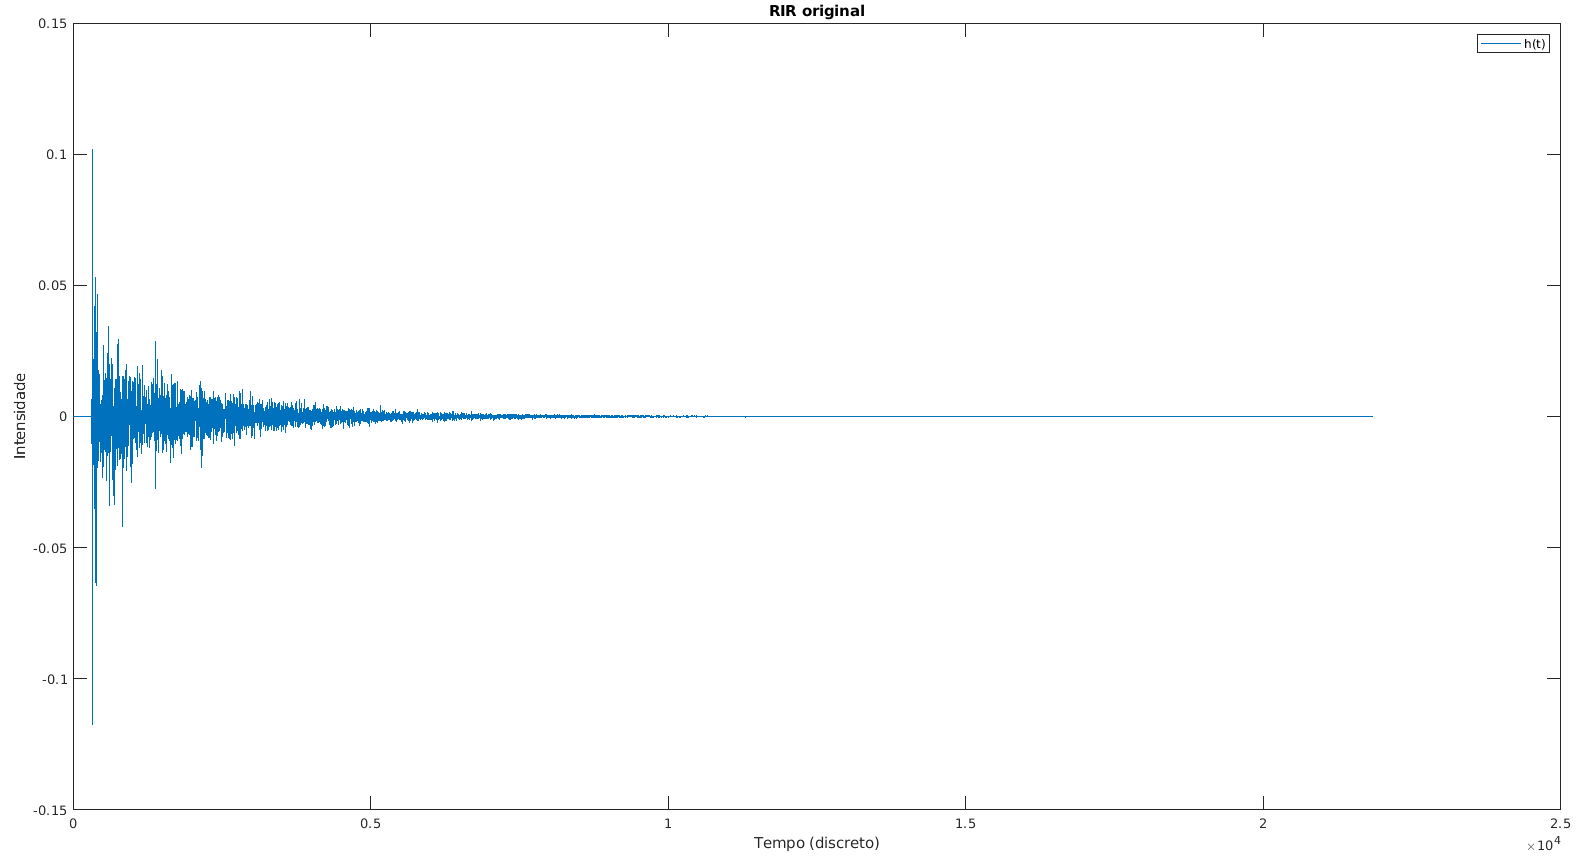
\includegraphics[scale=0.25]{rir-og-d1.png}
    \caption{RIR original.}
    \label{fig-a:rir-og-d1}
\end{figure} 

\begin{figure} [H]
    \centering
    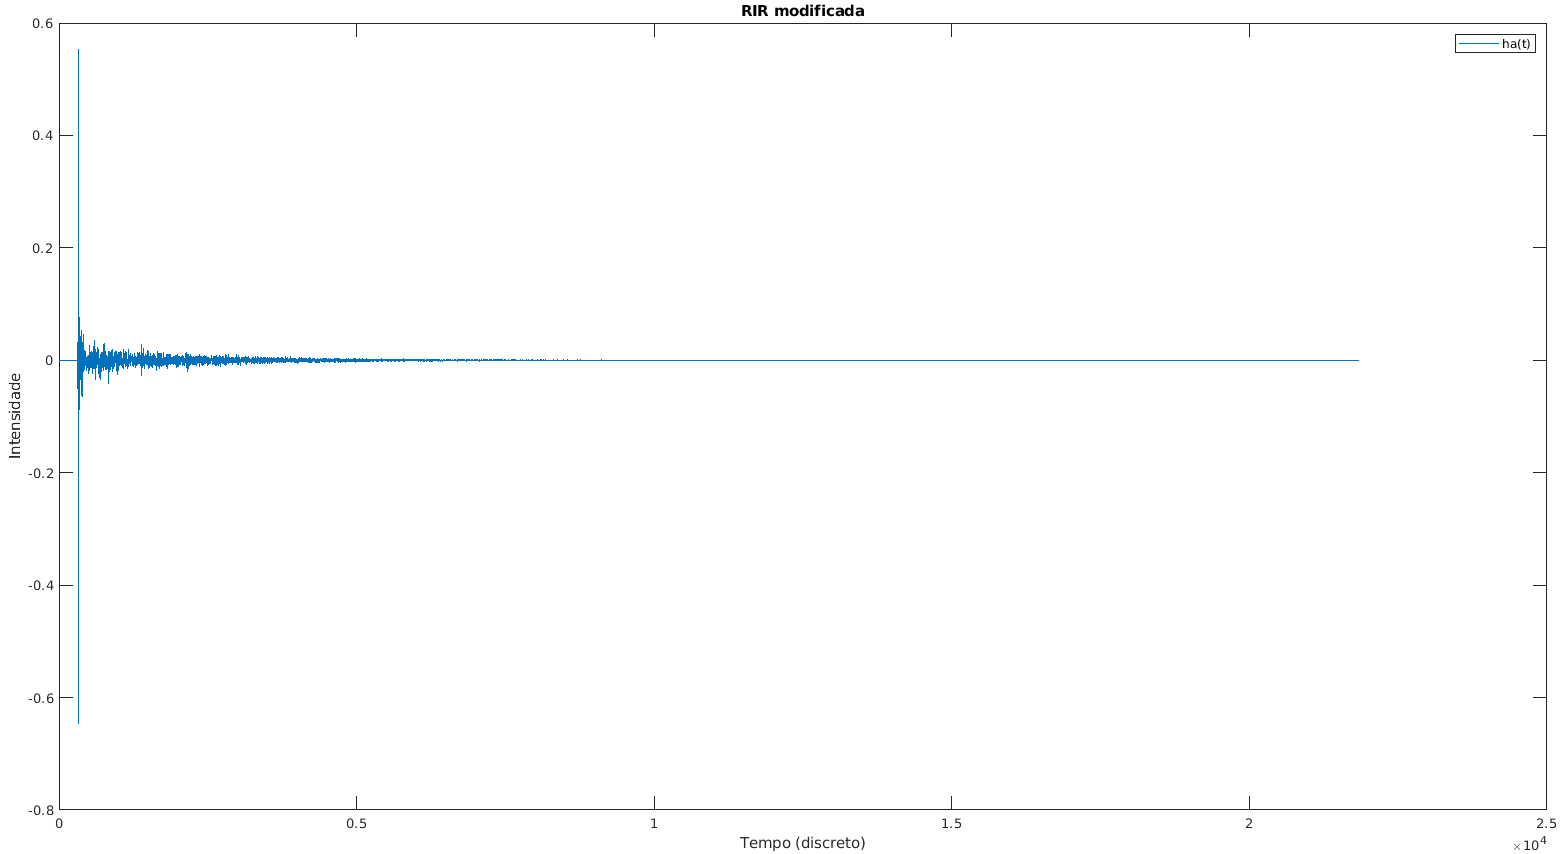
\includegraphics[scale=0.25]{rir-aug-d1.png}
    \caption{RIR simulada.}
    \label{fig-a:rir-aug-d1}
\end{figure} 

\begin{figure} [H]
    \centering
    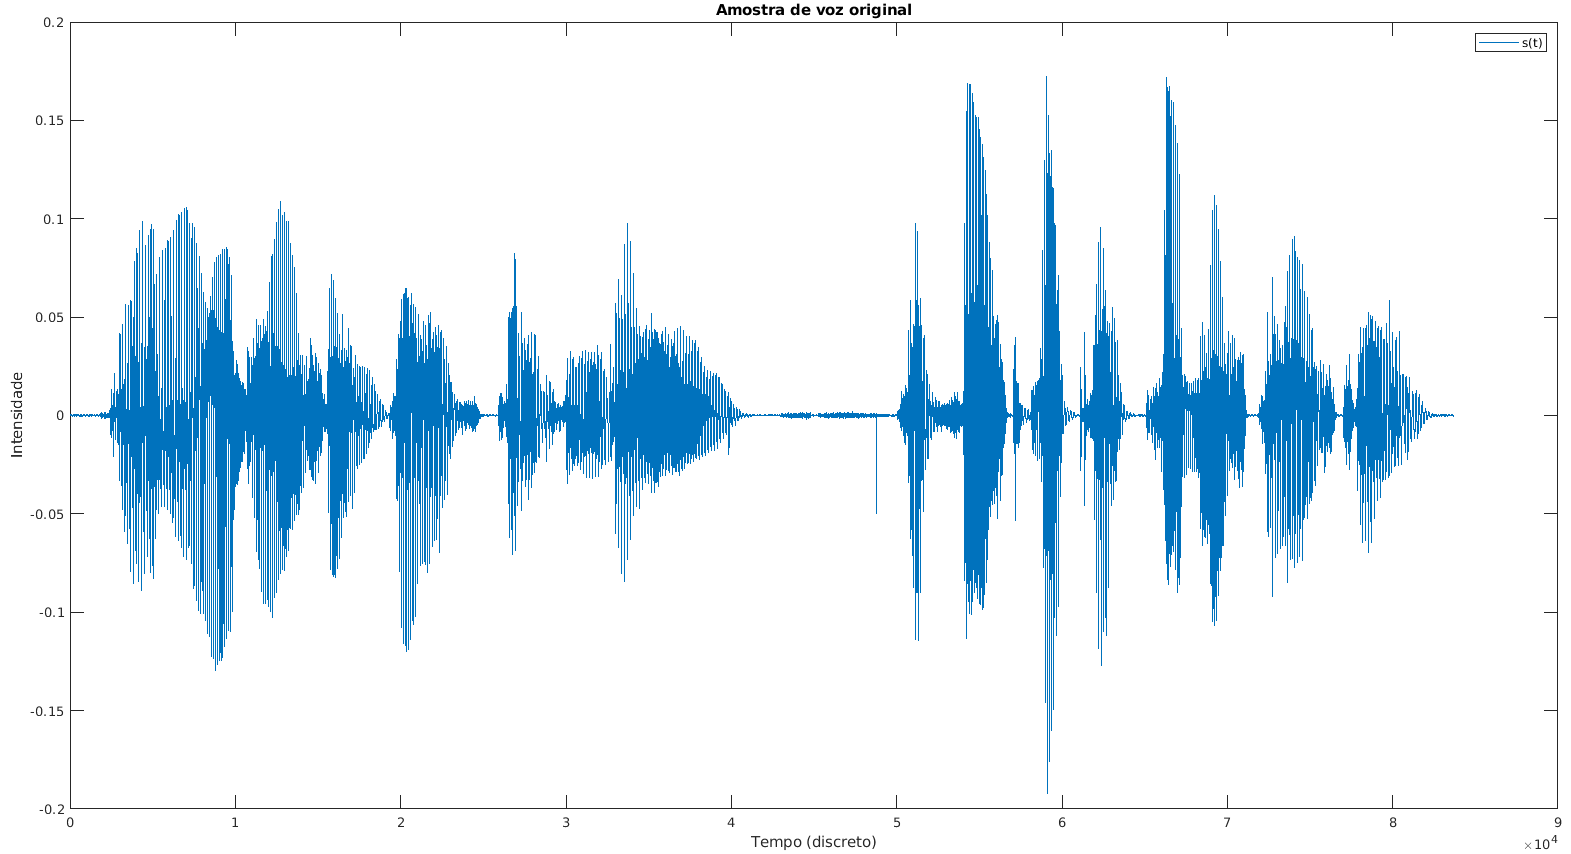
\includegraphics[scale=0.25]{voice-og-d1.png}
    \caption{Amostra de voz original.}
    \label{fig-a:voice-og-d1}
\end{figure} 

\begin{figure} [H]
    \centering
    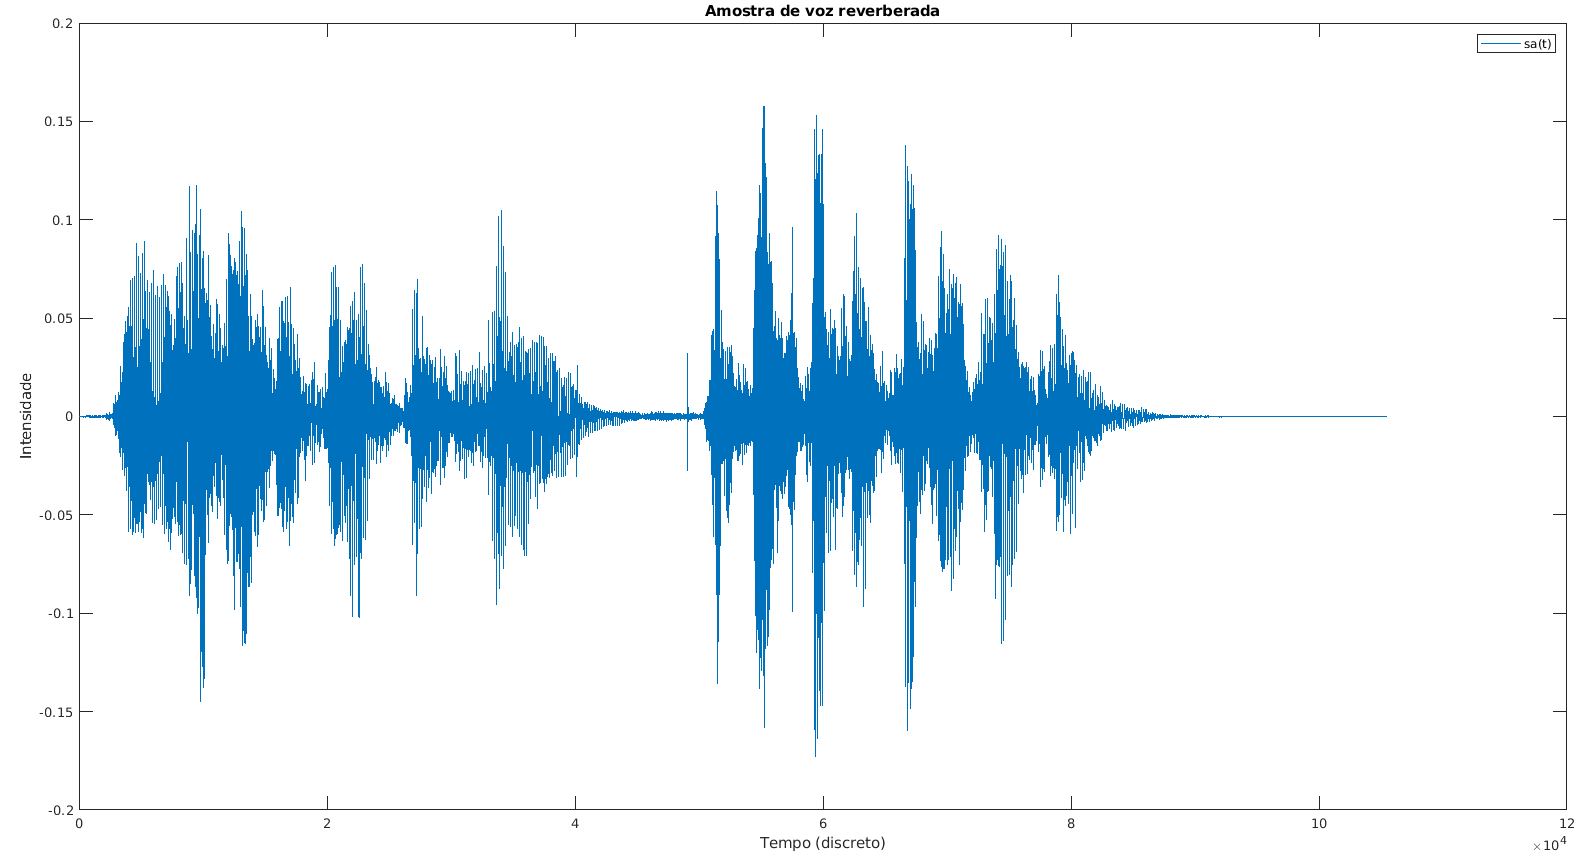
\includegraphics[scale=0.25]{voice-aug-d1.png}
    \caption{Amostra de voz reverberada com RIRSM.}
    \label{fig-a:voice-aug-d1}
\end{figure}

\pagebreak
{\Large \textbf{Exemplo D2}}

\begin{figure} [H]
    \centering
    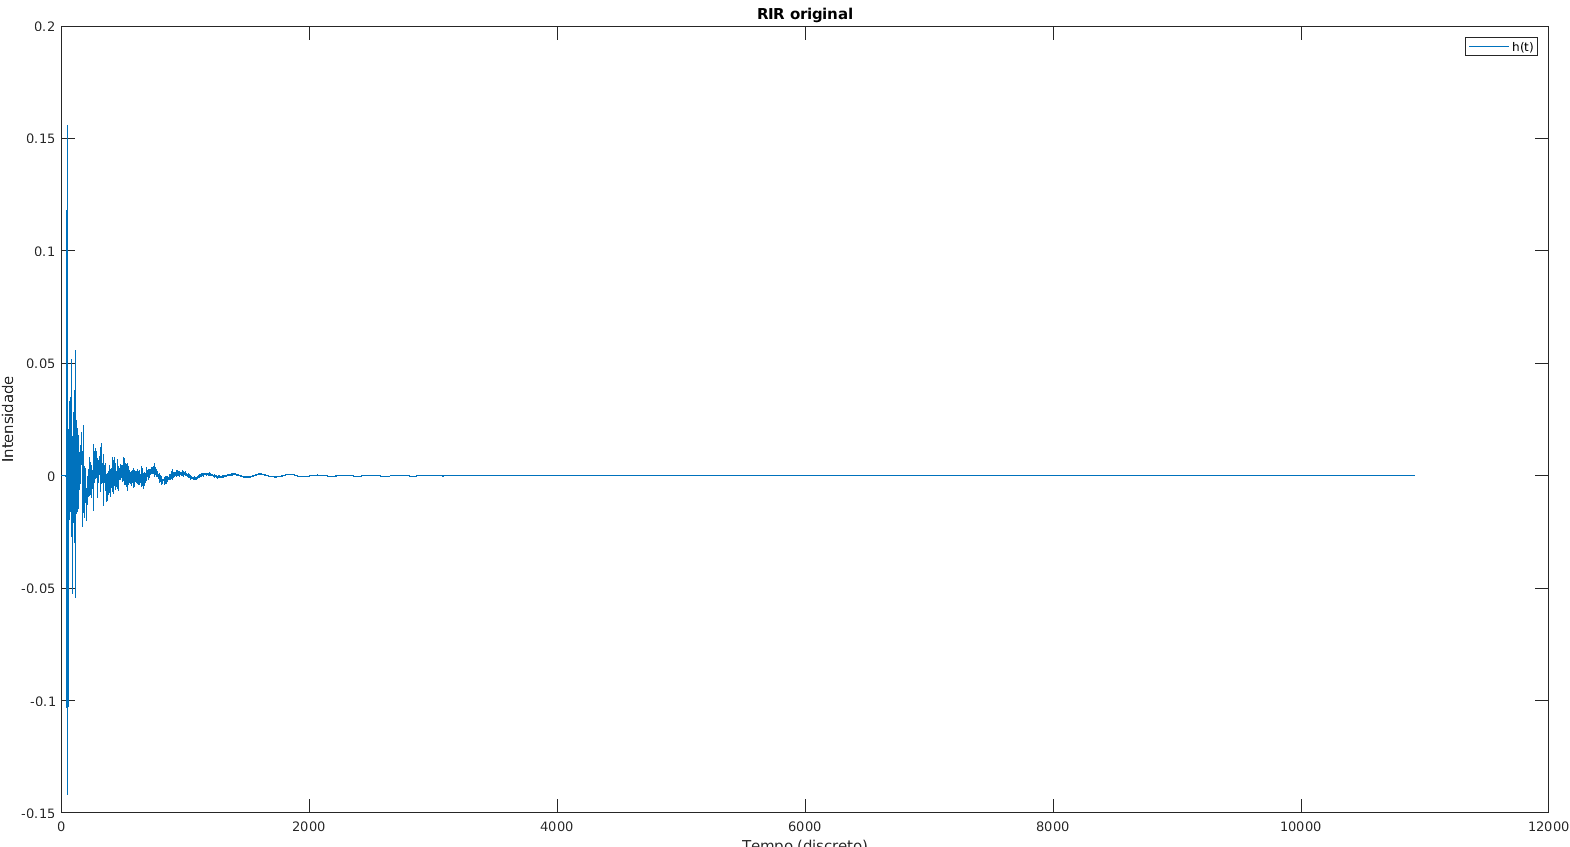
\includegraphics[scale=0.25]{rir-og-d2.png}
    \caption{RIR original.}
    \label{fig-a:rir-og-d2}
\end{figure} 

\begin{figure} [H]
    \centering
    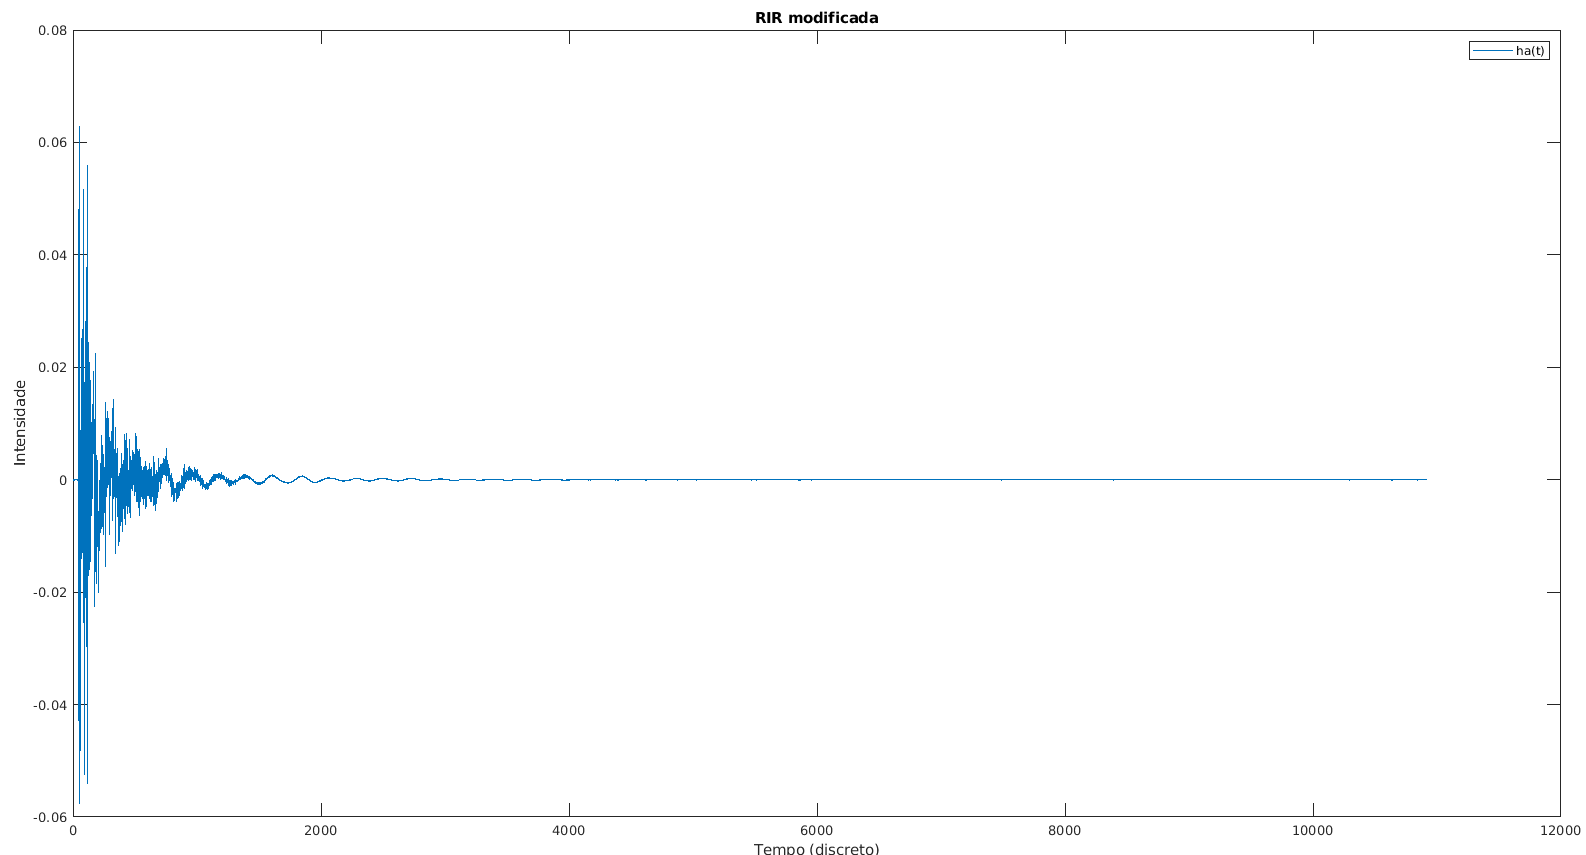
\includegraphics[scale=0.25]{rir-aug-d2.png}
    \caption{RIR simulada.}
    \label{fig-a:rir-aug-d2}
\end{figure} 

\begin{figure} [H]
    \centering
    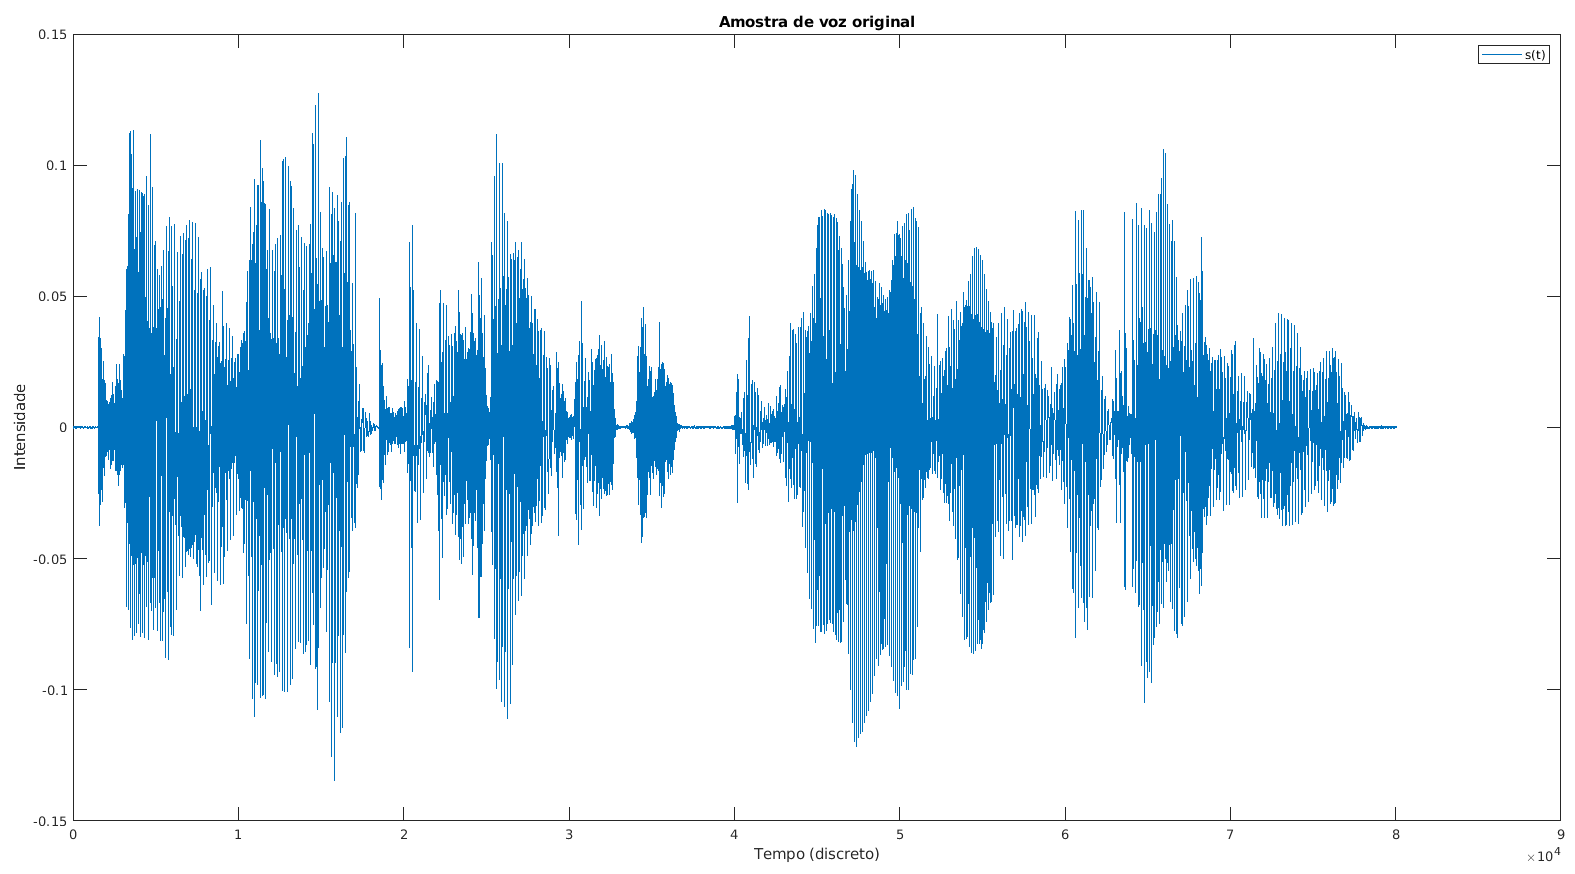
\includegraphics[scale=0.25]{voice-og-d2.png}
    \caption{Amostra de voz original.}
    \label{fig-a:voice-og-d2}
\end{figure} 

\begin{figure} [H]
    \centering
    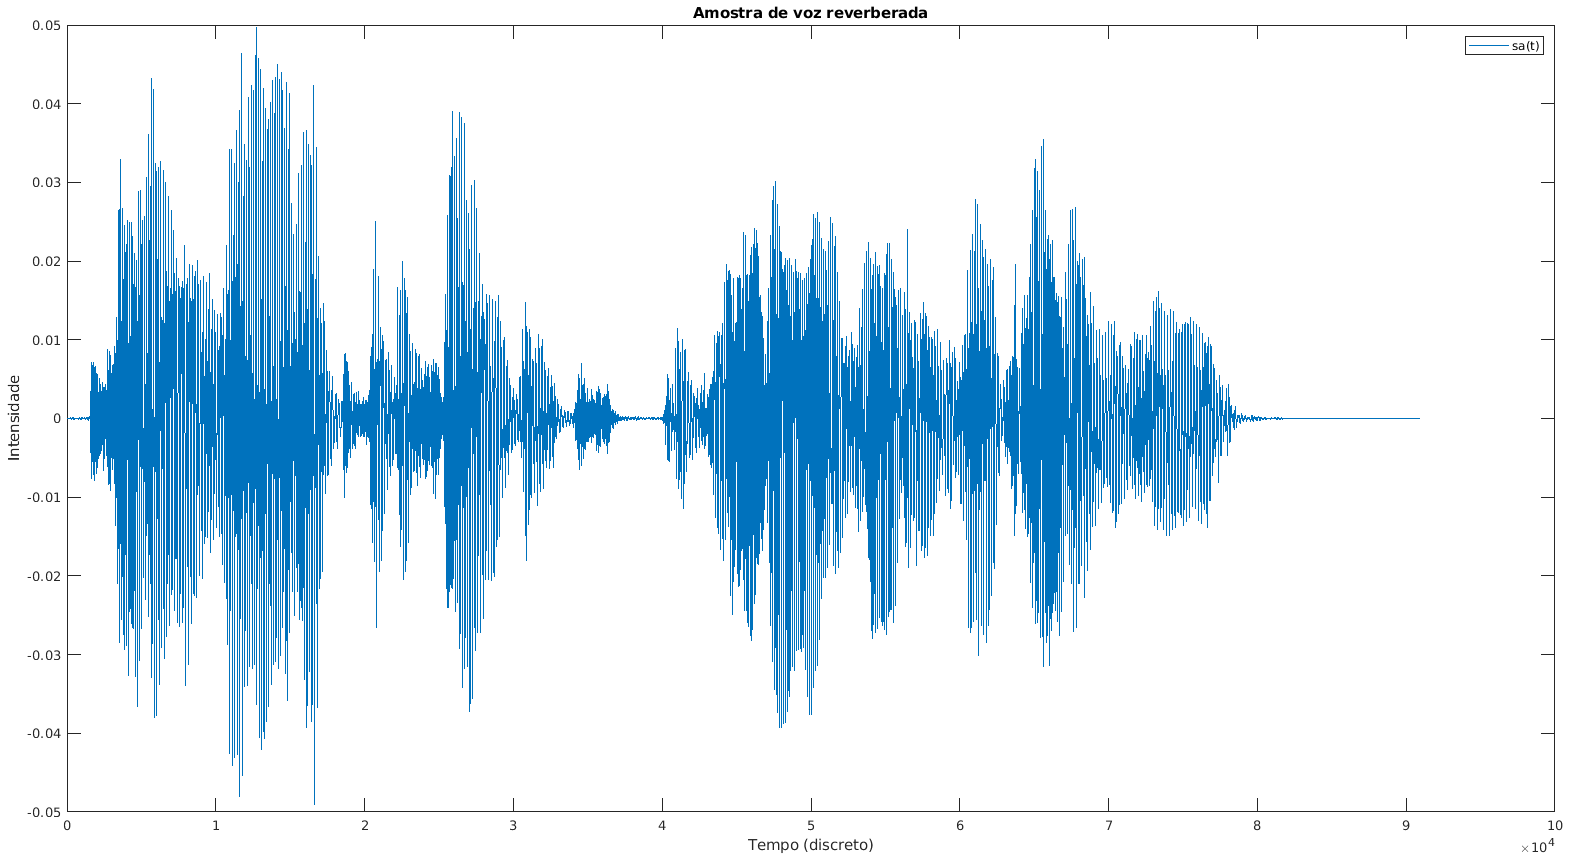
\includegraphics[scale=0.25]{voice-aug-d2.png}
    \caption{Amostra de voz reverberada com RIRSM.}
    \label{fig-a:voice-aug-d2}
\end{figure}

\pagebreak
{\Large \textbf{Exemplo D3}}

\begin{figure} [H]
    \centering
    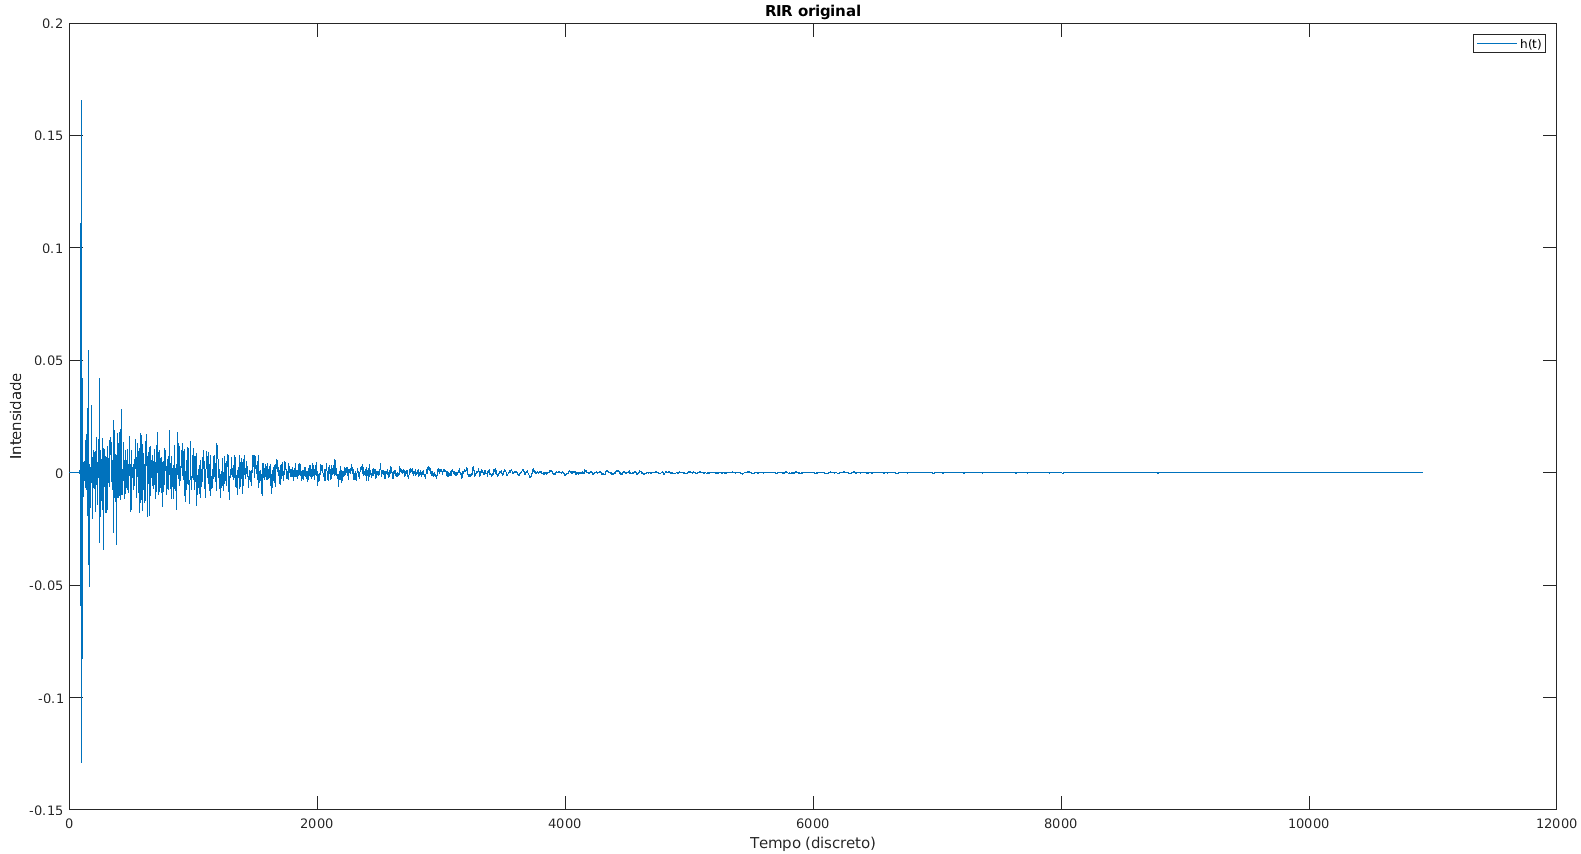
\includegraphics[scale=0.25]{rir-og-d3.png}
    \caption{RIR original.}
    \label{fig-a:rir-og-d3}
\end{figure} 

\begin{figure} [H]
    \centering
    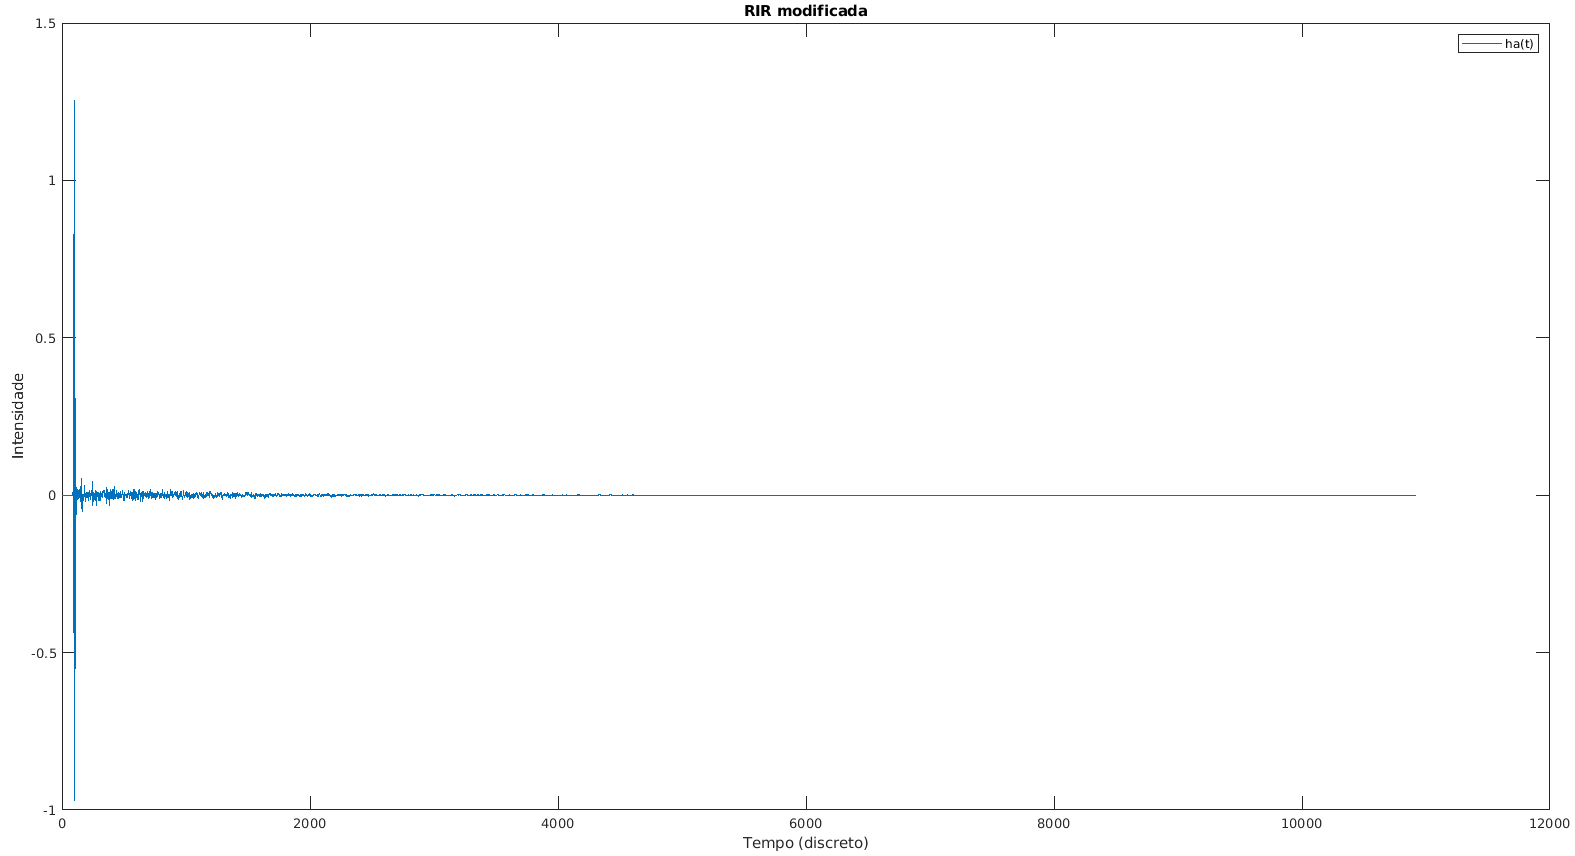
\includegraphics[scale=0.25]{rir-aug-d3.png}
    \caption{RIR simulada.}
    \label{fig-a:rir-aug-d3}
\end{figure} 

\begin{figure} [H]
    \centering
    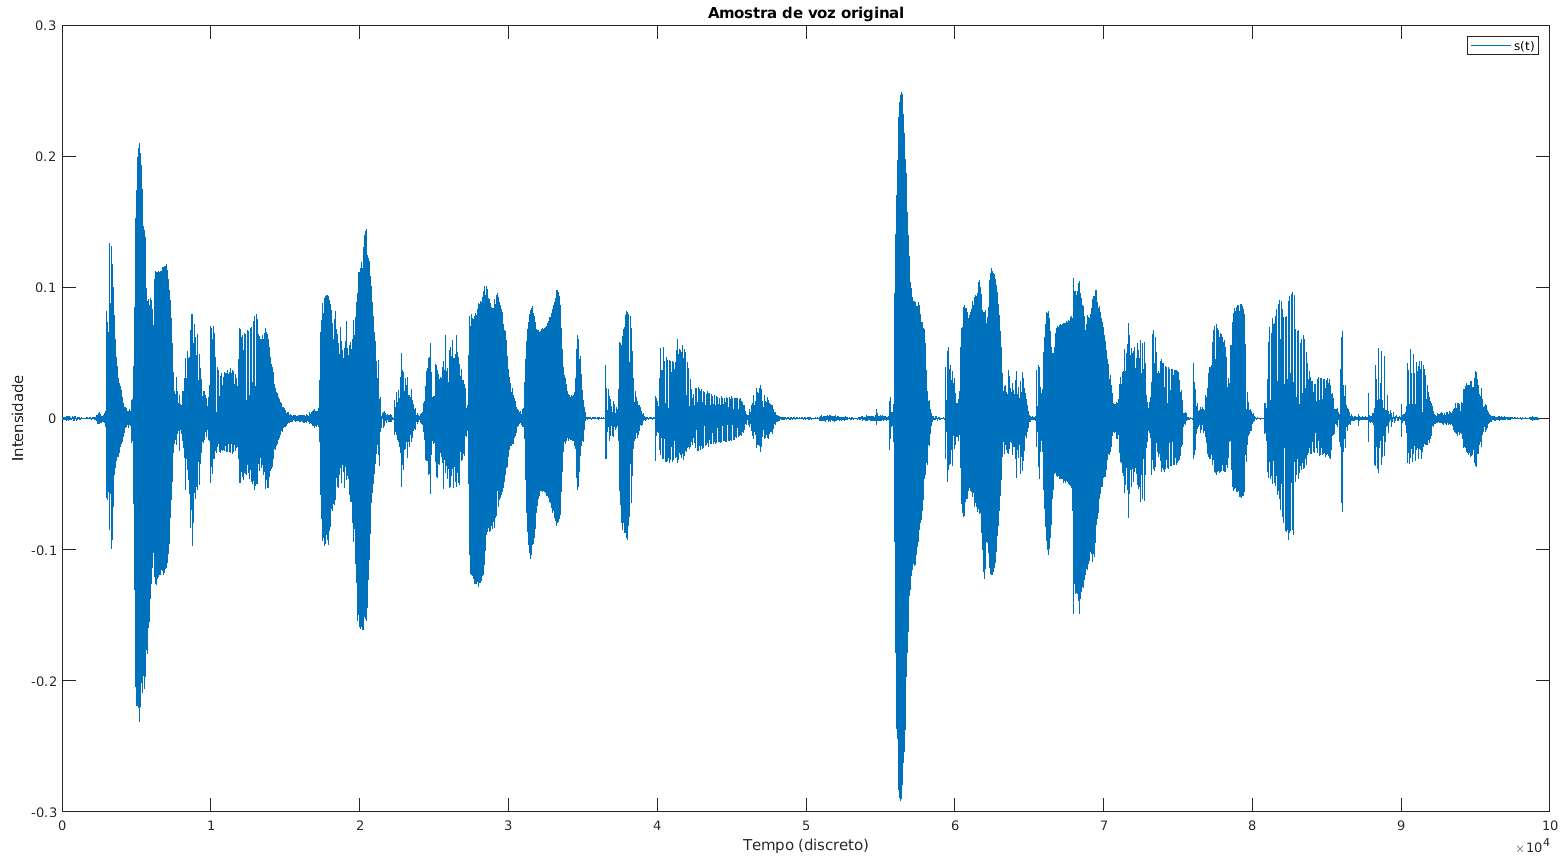
\includegraphics[scale=0.25]{voice-og-d3.png}
    \caption{Amostra de voz original.}
    \label{fig-a:voice-og-d3}
\end{figure} 

\begin{figure} [H]
    \centering
    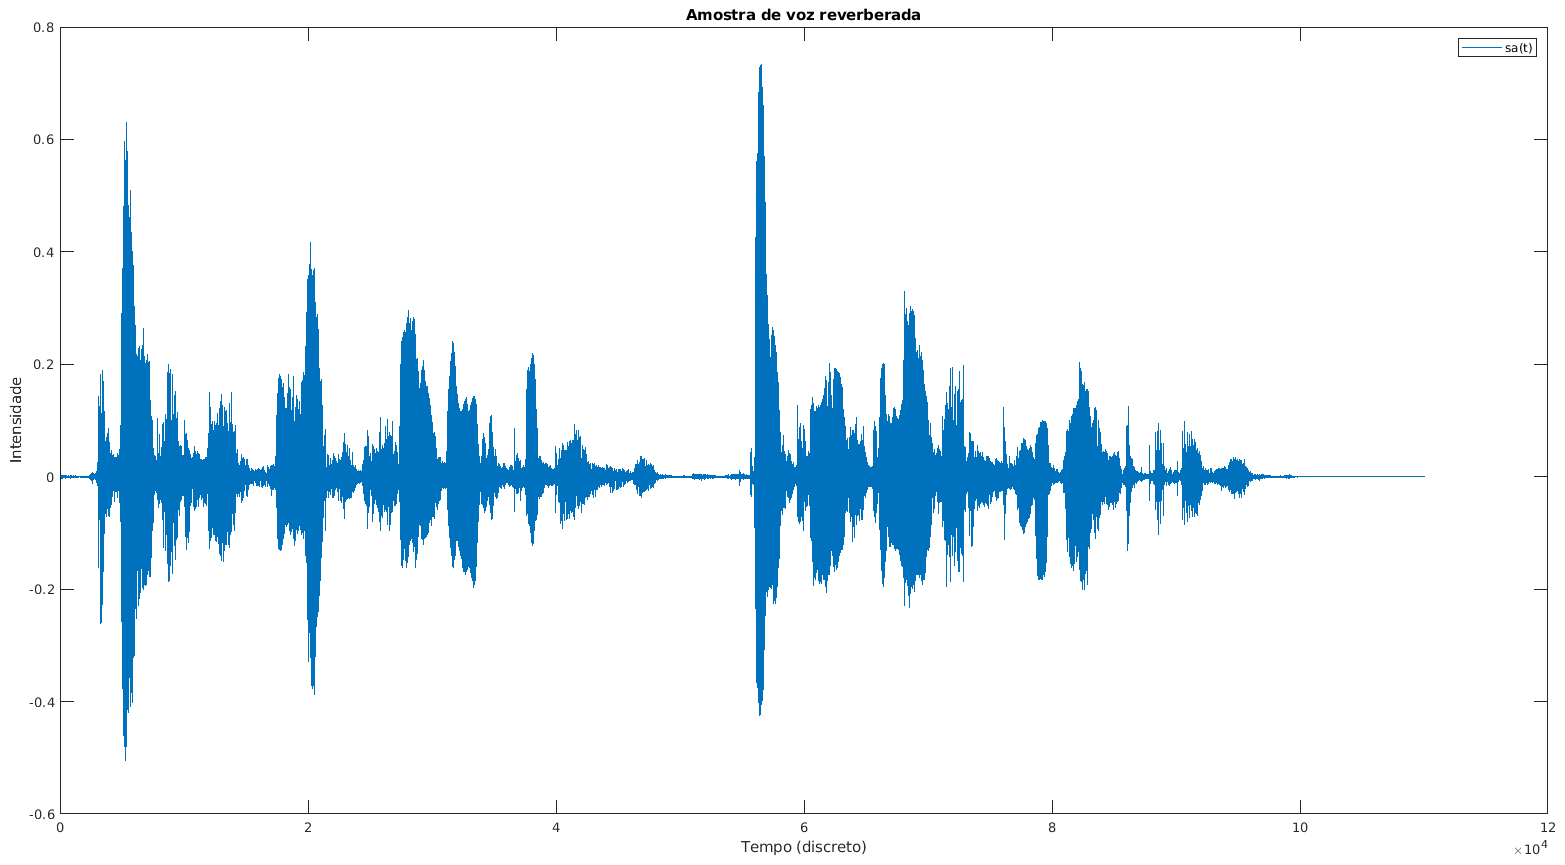
\includegraphics[scale=0.25]{voice-aug-d3.png}
    \caption{Amostra de voz reverberada com RIRSM.}
    \label{fig-a:voice-aug-d3}
\end{figure}

\pagebreak
\section{\textit{Data Augmentation de T60}}

\begin{table} [H]
    \centering
    \caption{Exemplos de DA de T60 gerados.}
    \label{tbl-a:da-t60}
    \begin{tabular}{c|c|c|c}

        \textbf{Exemplo} & 
        \textbf{Sala RIR} & 
        \textbf{Distância (m)} &
        \textbf{Amostra de Voz} \\
        \hline 

        T1 & lecture & 7.1 & M2-T1 \\
        T2 & booth & 1 & H1-T2 \\
        T3 & office & 2 & H2-T2 \\

    \end{tabular}
    \bigbreak
    \bigbreak
    \begin{tabular}{c|c|c|c|c}

        \textbf{Exemplo} & 
        \textbf{$T60_{org}$ (s)} & 
        \textbf{$T60_{alvo}$ (s)} &
        \textbf{$T60_{res}$ (s)} & 
        \textbf{$\rho$ (\%)} \\
        \hline 

        T1 & 1,38 & 1,15 & 1,01 & 12.1 \\
        T2 & 1,01 & 1,88 & 1,89 & 0,5 \\
        T3 & 0,75 & 0,61 & 0,60 & 1,6 \\

    \end{tabular}
\end{table}

\pagebreak
{\Large \textbf{Exemplo T1}}

\begin{figure} [H]
    \centering
    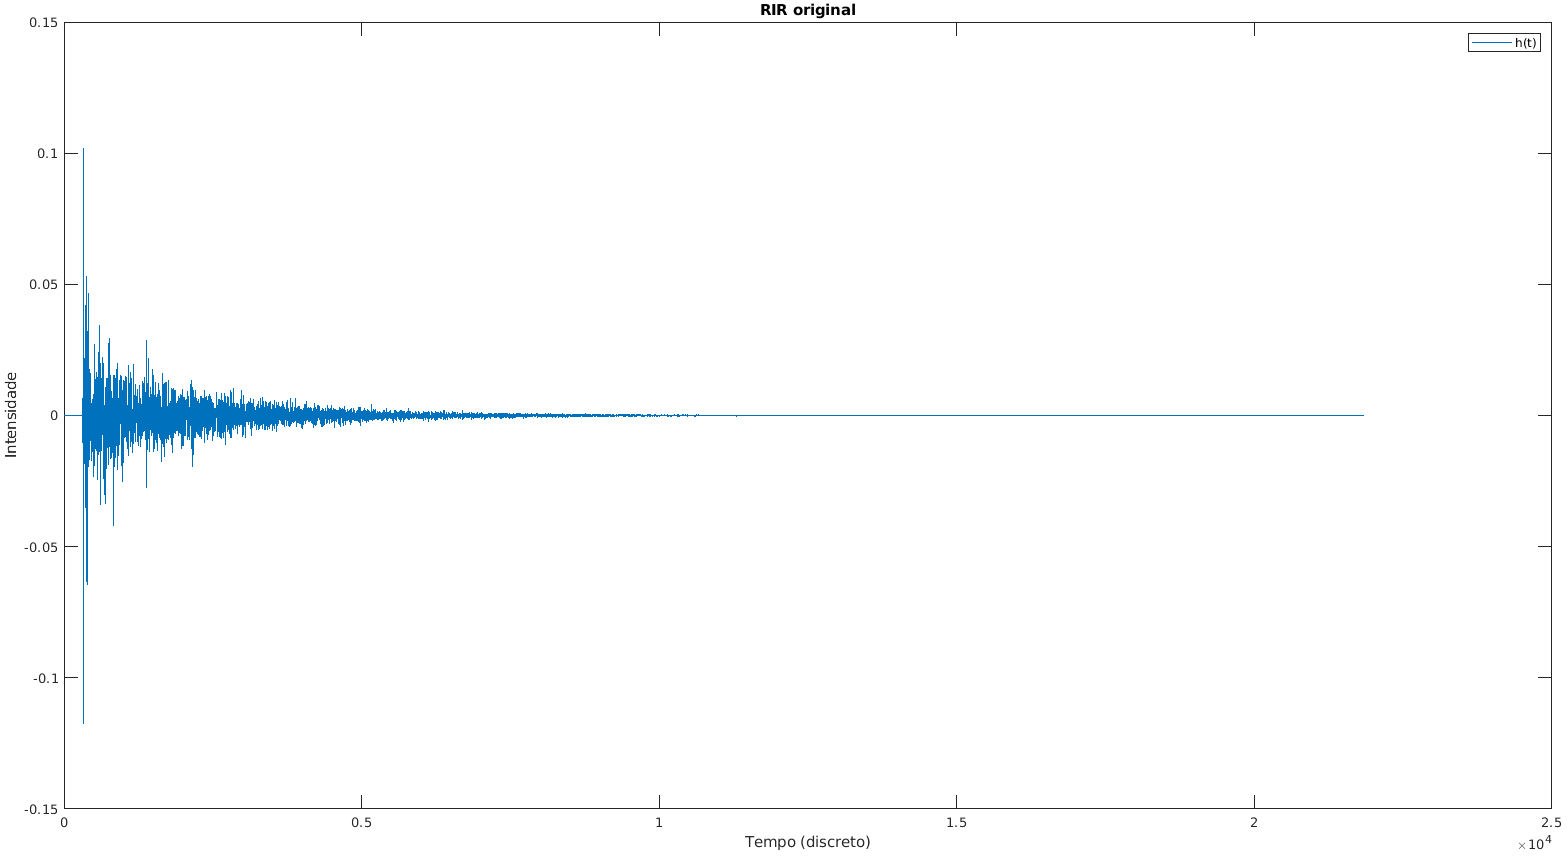
\includegraphics[scale=0.25]{rir-og-t1.png}
    \caption{RIR original.}
    \label{fig-a:rir-og-t1}
\end{figure} 

\begin{figure} [H]
    \centering
    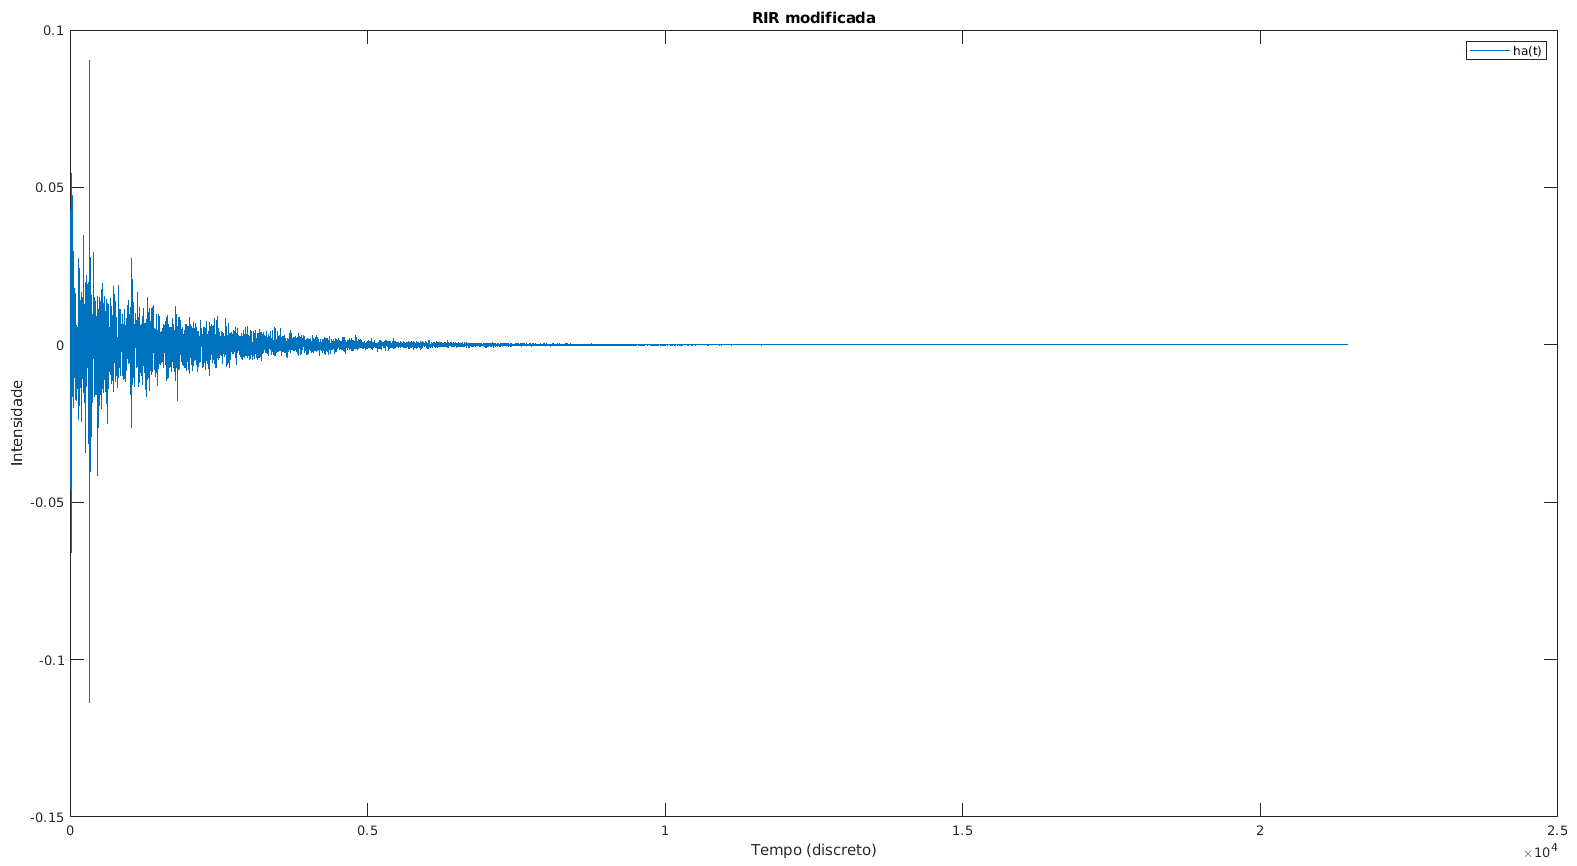
\includegraphics[scale=0.25]{rir-aug-t1.png}
    \caption{RIR simulada.}
    \label{fig-a:rir-aug-t1}
\end{figure} 

\begin{figure} [H]
    \centering
    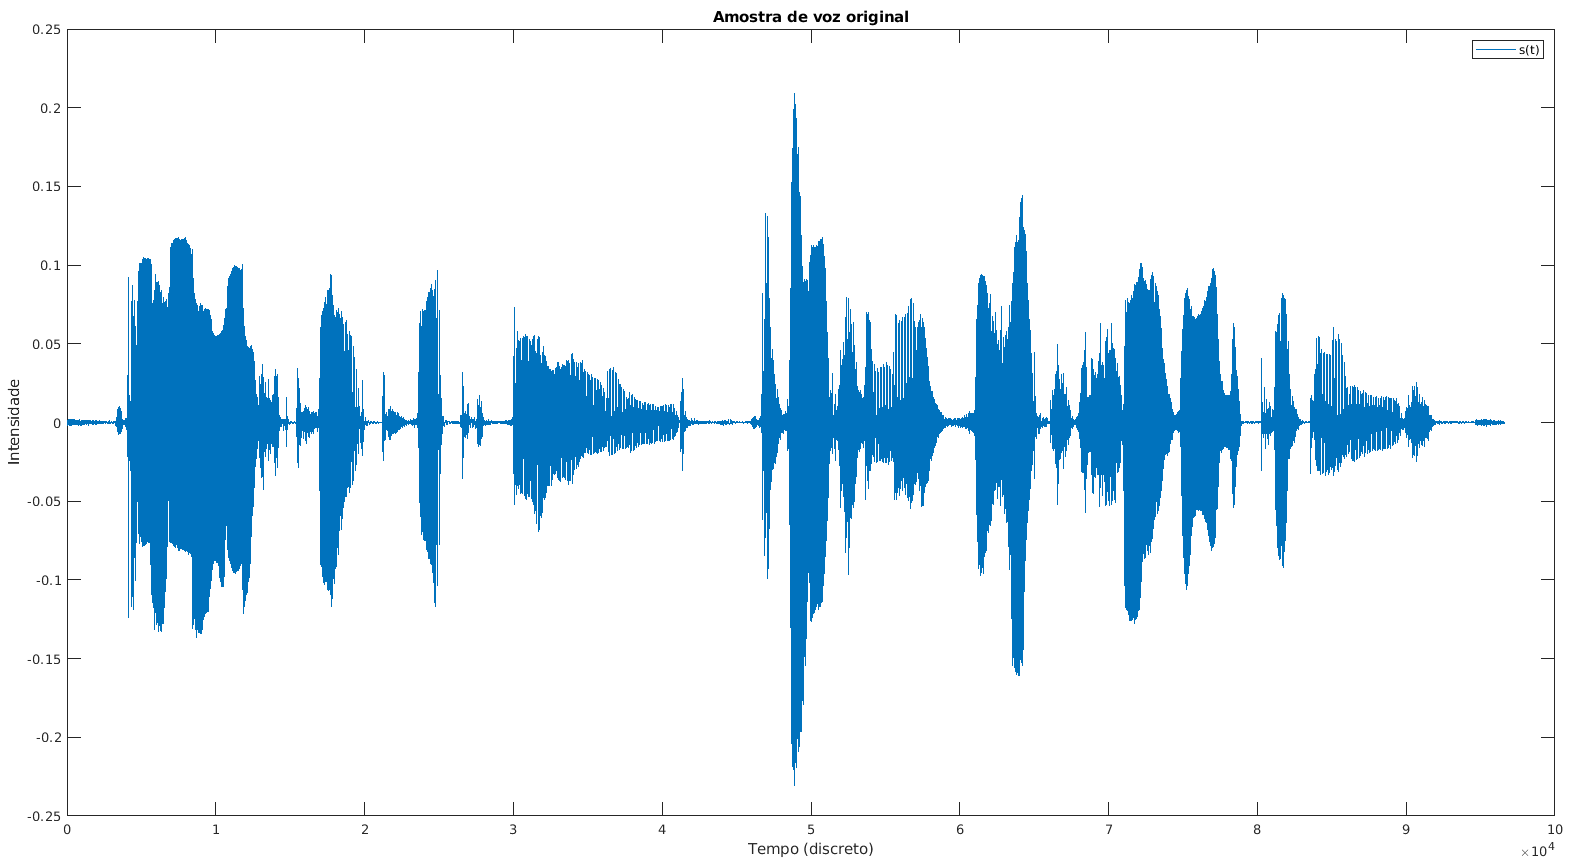
\includegraphics[scale=0.25]{voice-og-t1.png}
    \caption{Amostra de voz original.}
    \label{fig-a:voice-og-t1}
\end{figure} 

\begin{figure} [H]
    \centering
    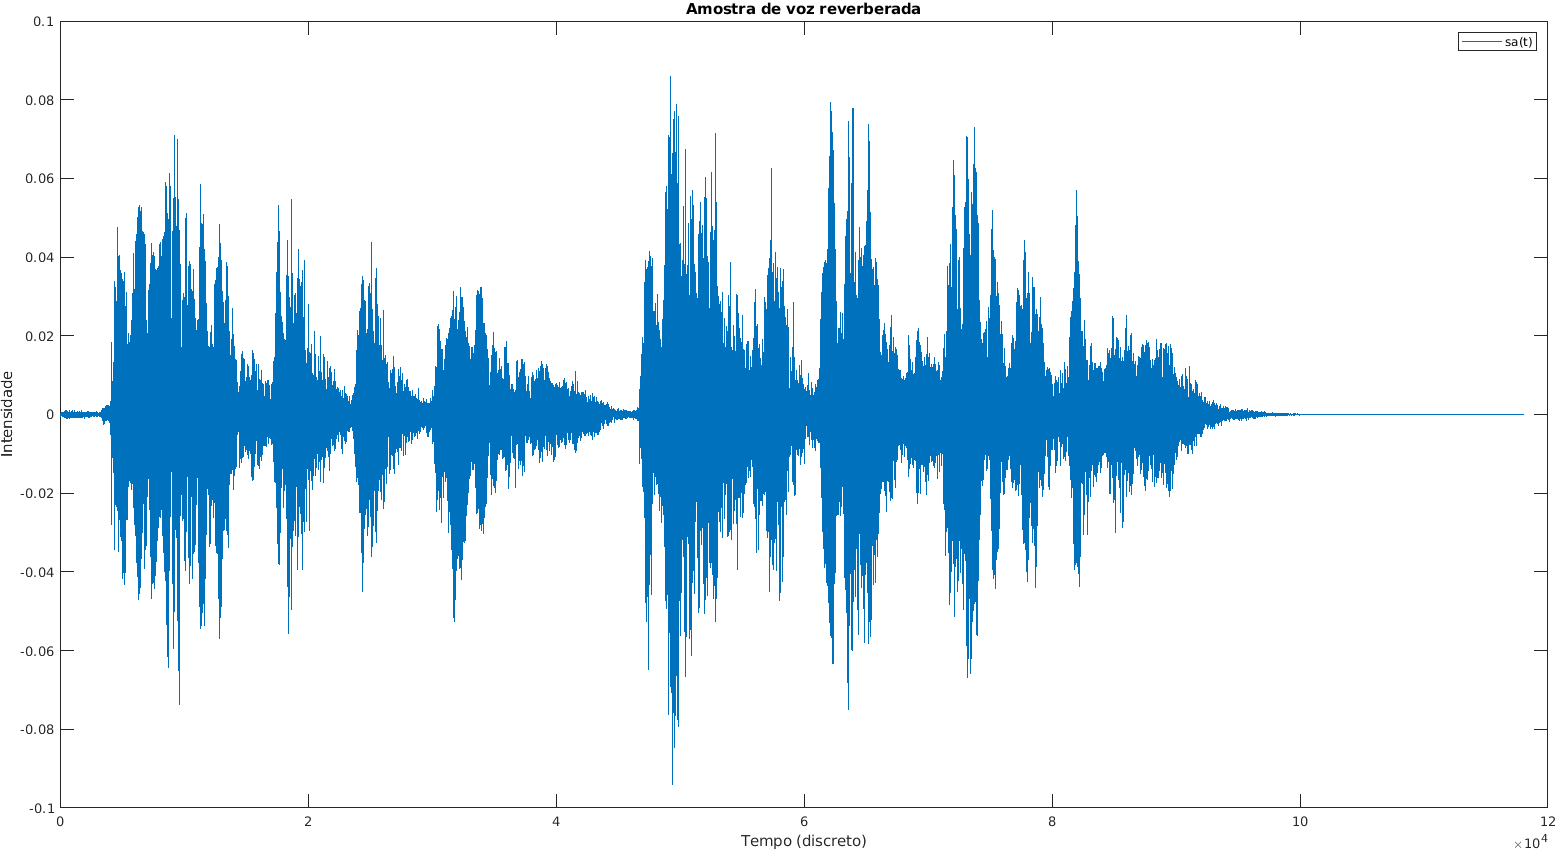
\includegraphics[scale=0.25]{voice-aug-t1.png}
    \caption{Amostra de voz reverberada com RIRSM.}
    \label{fig-a:voice-aug-t1}
\end{figure}

\pagebreak
{\Large \textbf{Exemplo T2}}

\begin{figure} [H]
    \centering
    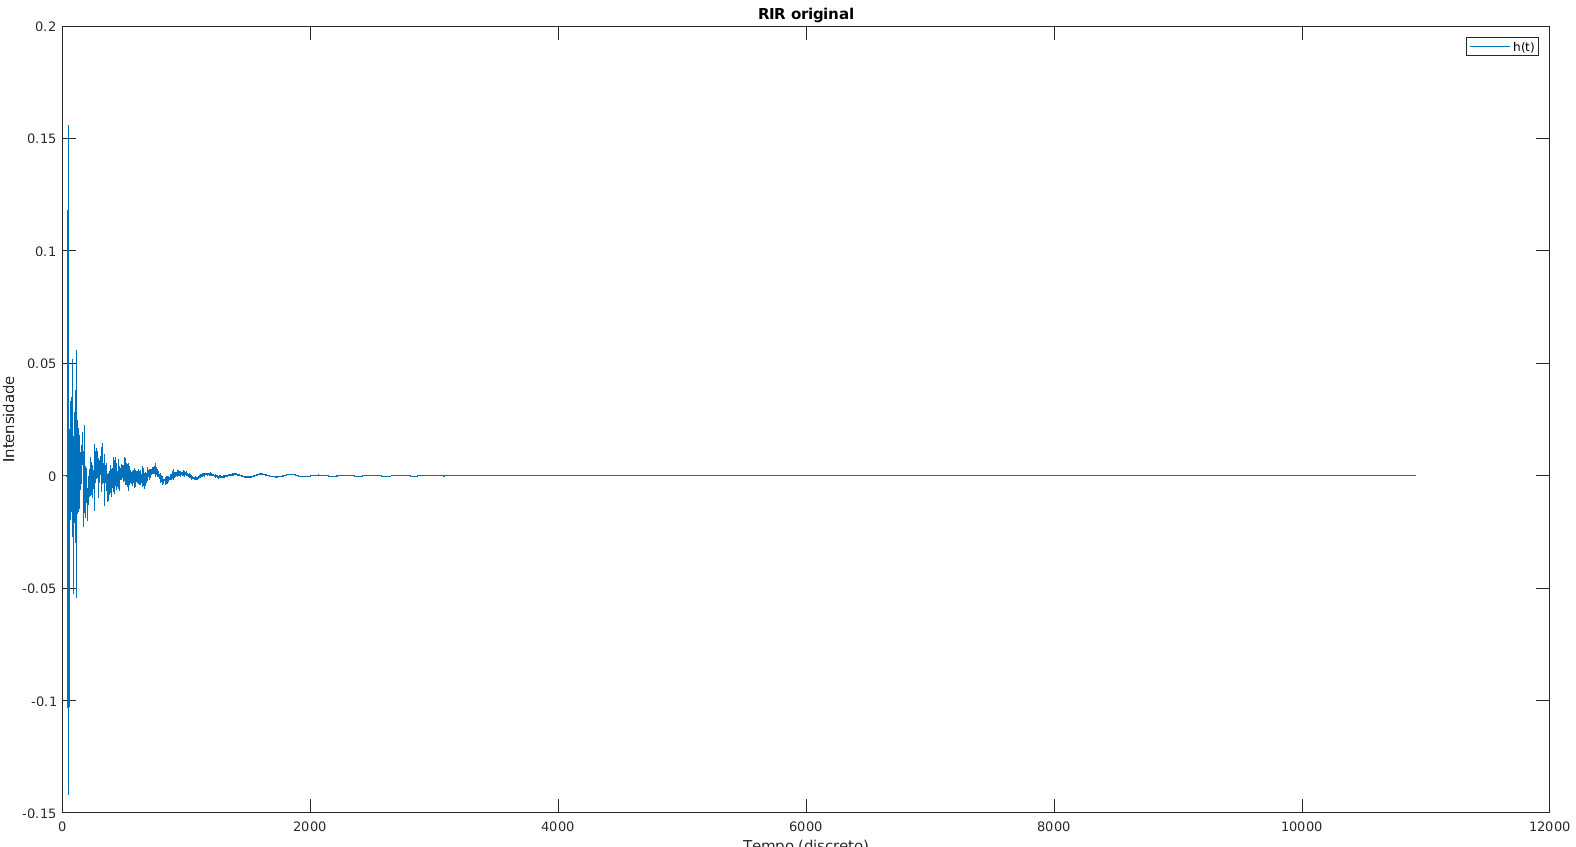
\includegraphics[scale=0.25]{rir-og-t2.png}
    \caption{RIR original.}
    \label{fig-a:rir-og-t2}
\end{figure} 

\begin{figure} [H]
    \centering
    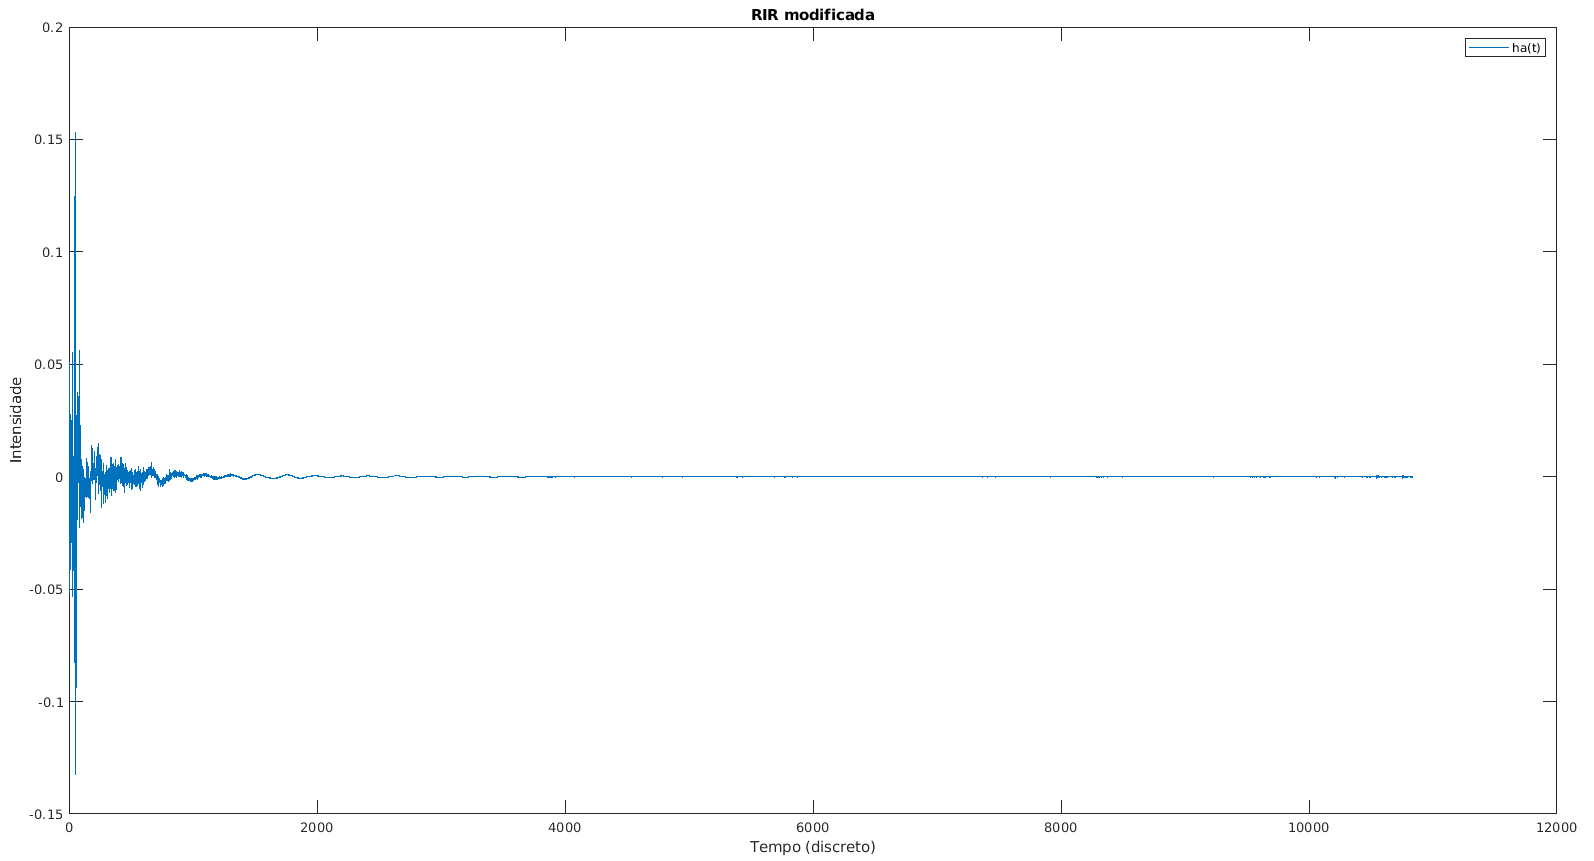
\includegraphics[scale=0.25]{rir-aug-t2.png}
    \caption{RIR simulada.}
    \label{fig-a:rir-aug-t2}
\end{figure} 

\begin{figure} [H]
    \centering
    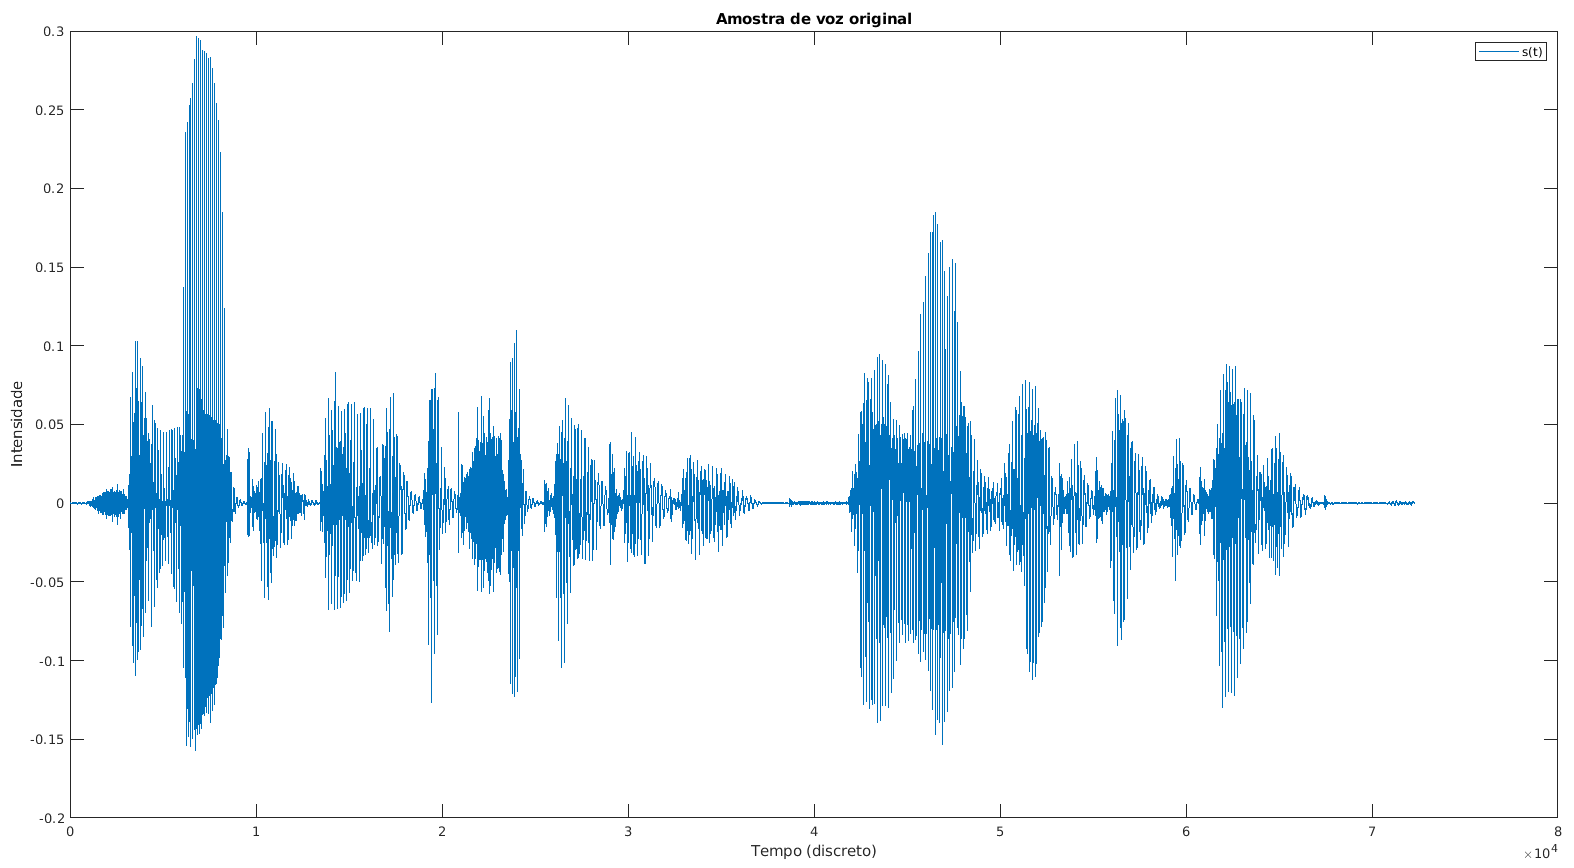
\includegraphics[scale=0.25]{voice-og-t2.png}
    \caption{Amostra de voz original.}
    \label{fig-a:voice-og-t2}
\end{figure} 

\begin{figure} [H]
    \centering
    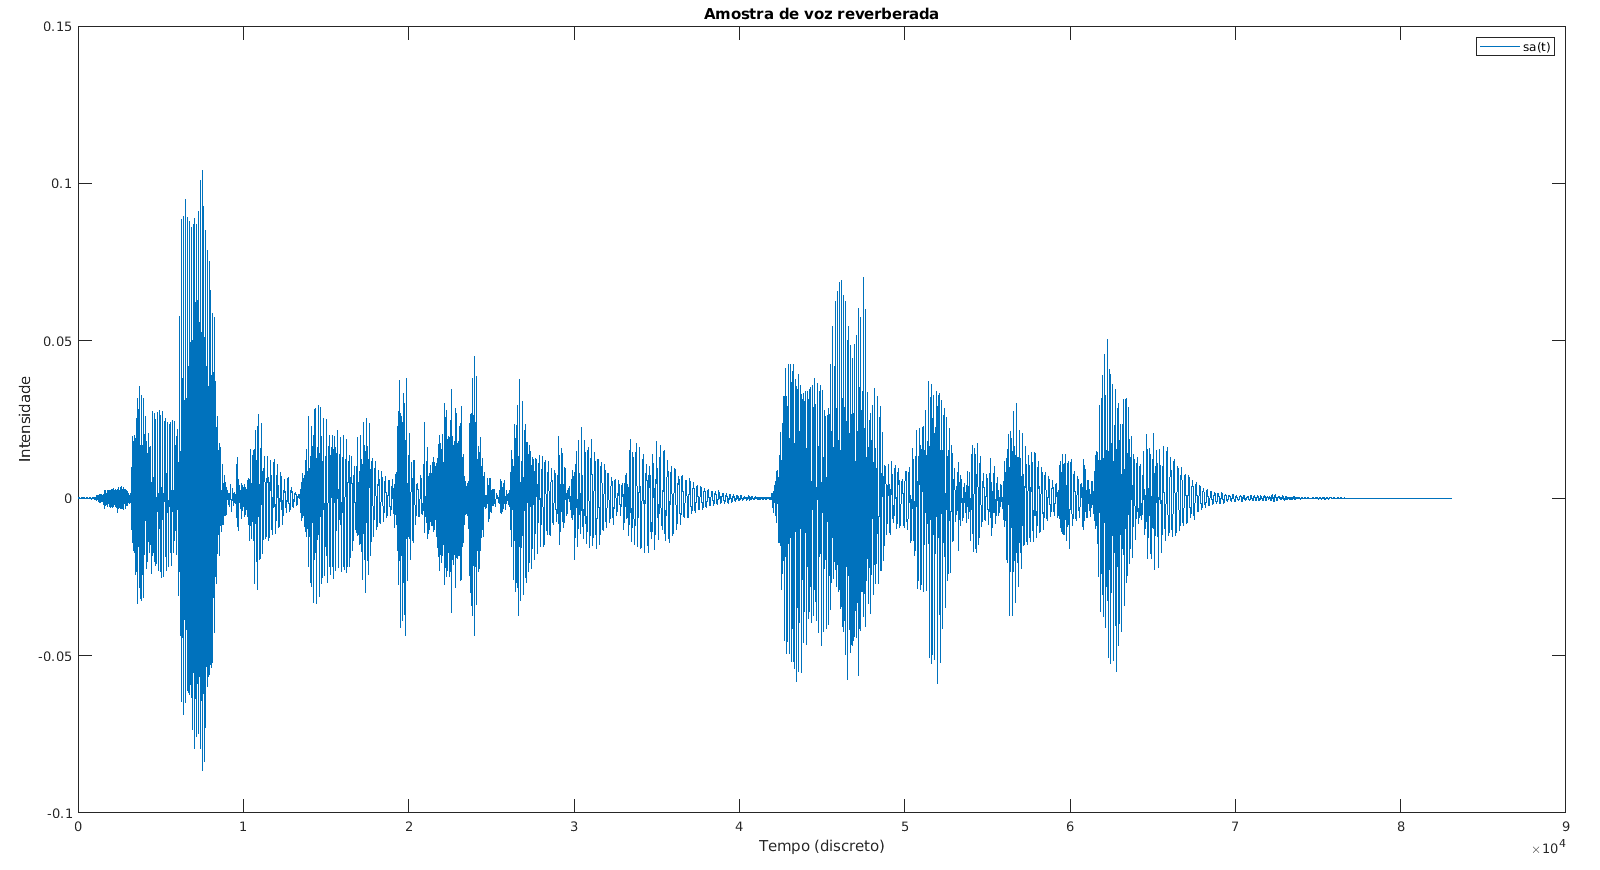
\includegraphics[scale=0.25]{voice-aug-t2.png}
    \caption{Amostra de voz reverberada com RIRSM.}
    \label{fig-a:voice-aug-t2}
\end{figure}

\pagebreak
{\Large \textbf{Exemplo T3}}

\begin{figure} [H]
    \centering
    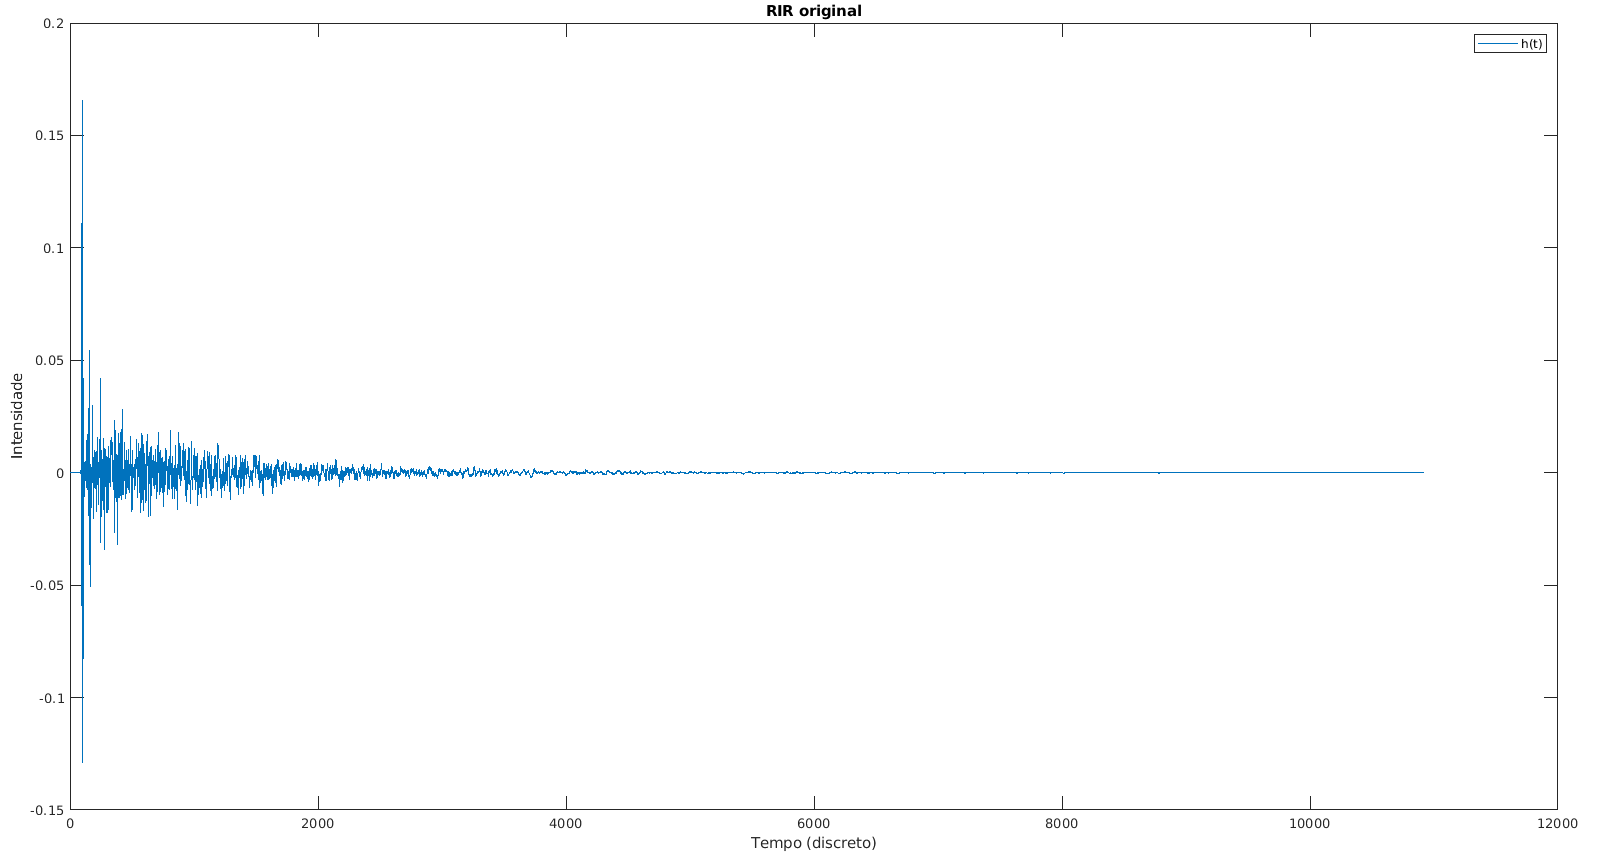
\includegraphics[scale=0.25]{rir-og-t3.png}
    \caption{RIR original.}
    \label{fig-a:rir-og-t3}
\end{figure} 

\begin{figure} [H]
    \centering
    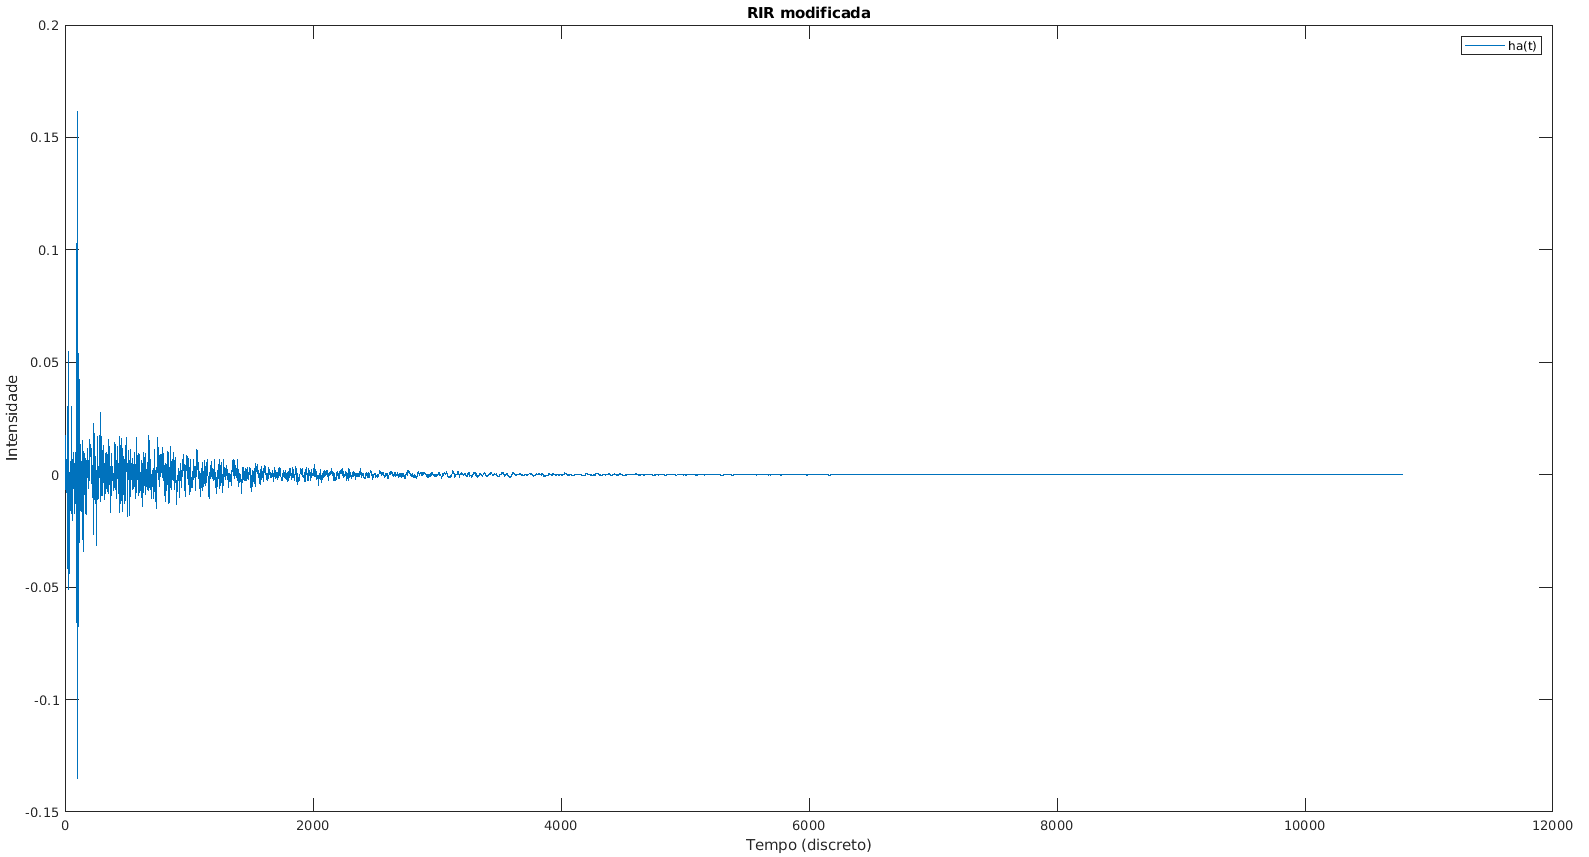
\includegraphics[scale=0.25]{rir-aug-t3.png}
    \caption{RIR simulada.}
    \label{fig-a:rir-aug-t3}
\end{figure} 

\begin{figure} [H]
    \centering
    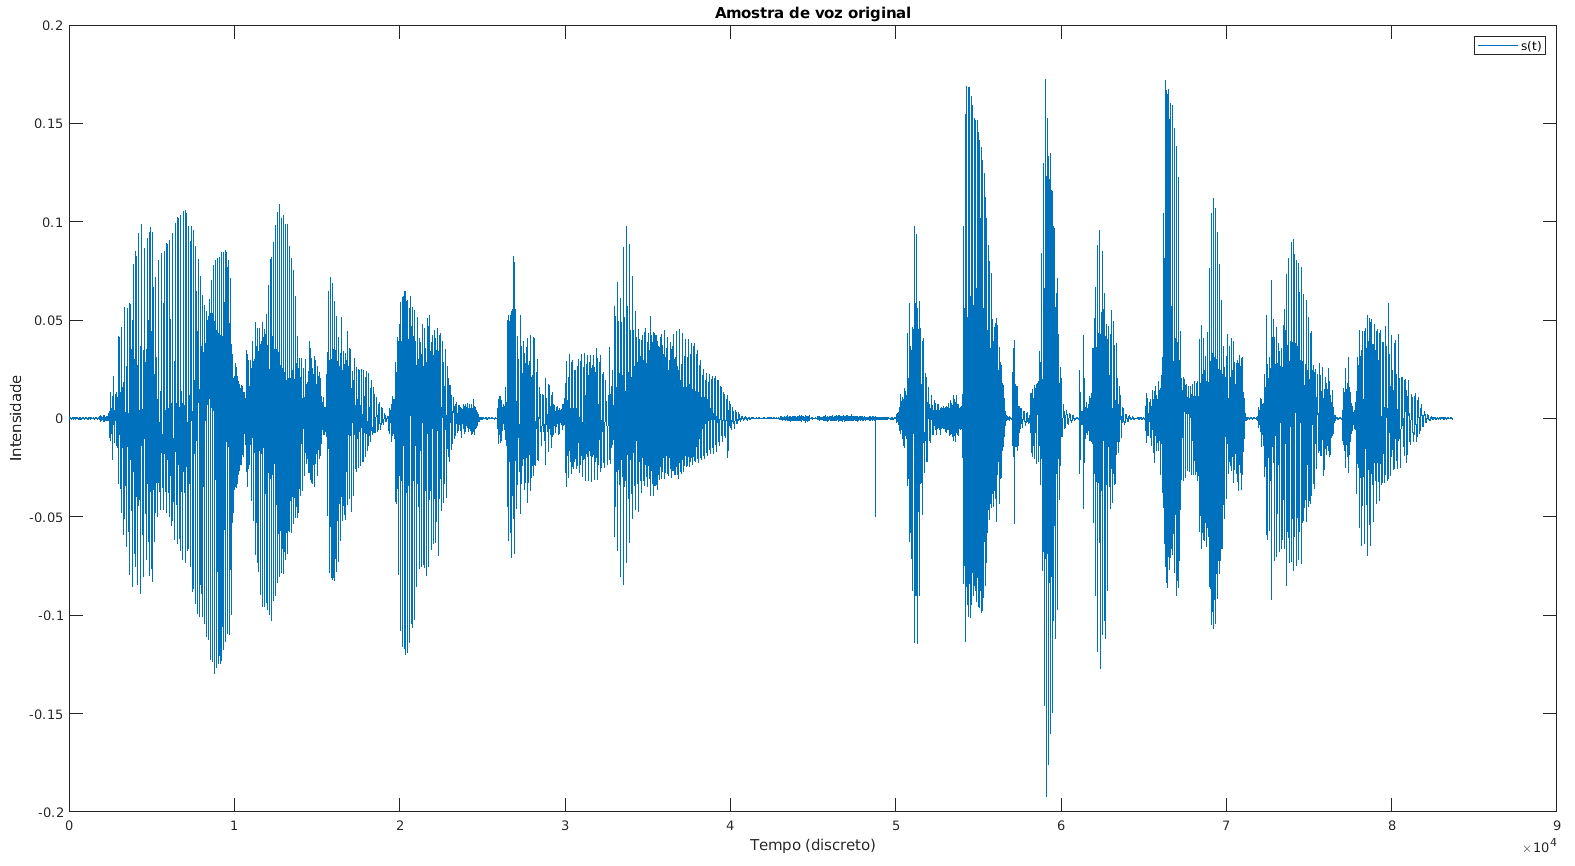
\includegraphics[scale=0.25]{voice-og-t3.png}
    \caption{Amostra de voz original.}
    \label{fig-a:voice-og-t3}
\end{figure} 

\begin{figure} [H]
    \centering
    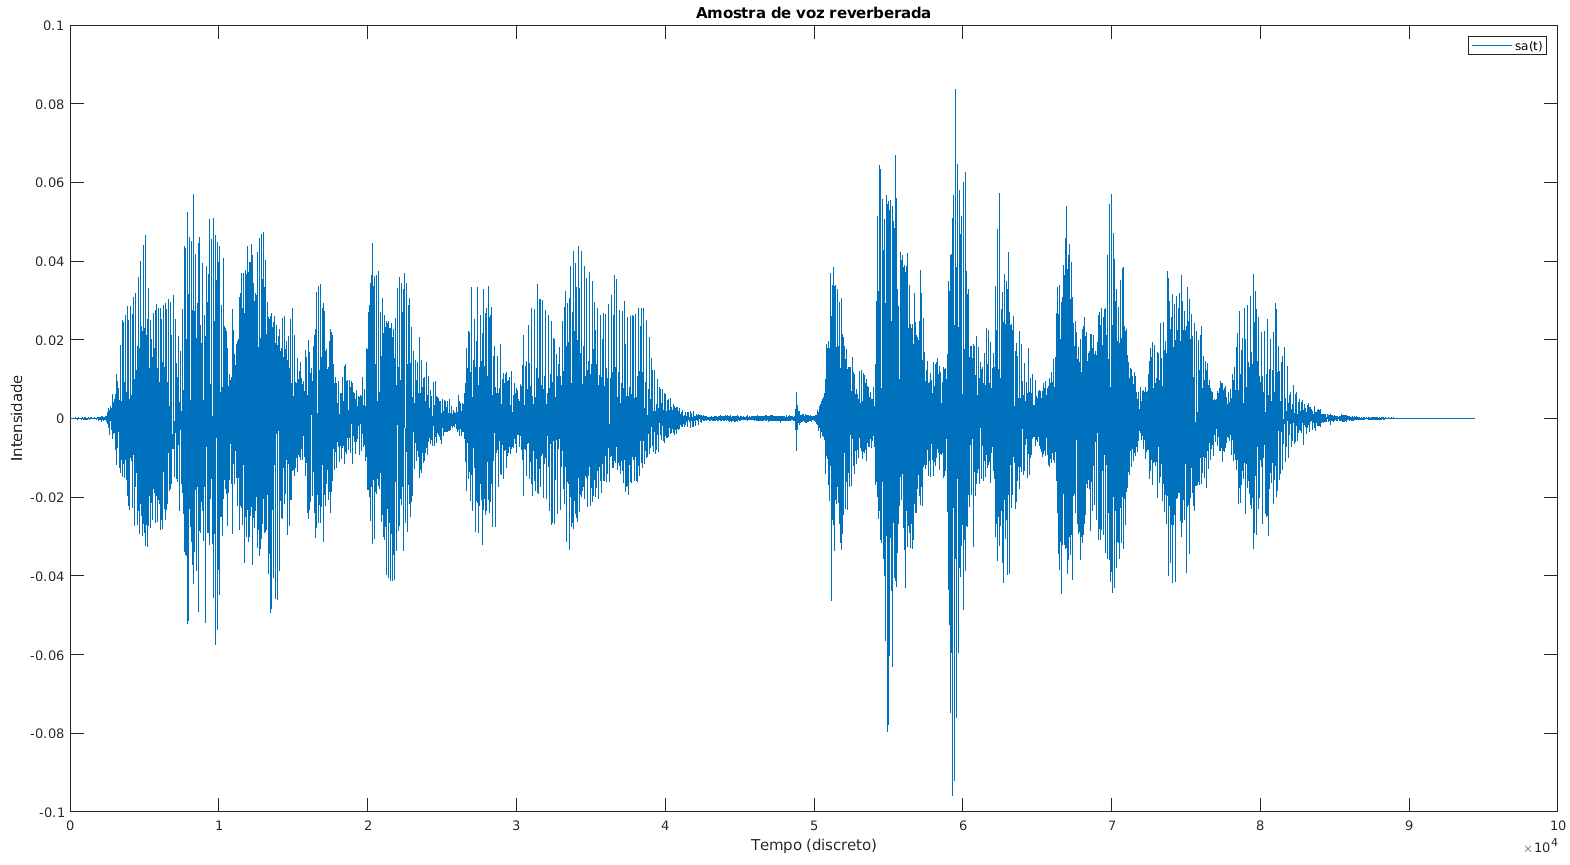
\includegraphics[scale=0.25]{voice-aug-t3.png}
    \caption{Amostra de voz reverberada com RIRSM.}
    \label{fig-a:voice-aug-t3}
\end{figure}

\pagebreak
\section{\textit{Data Augmentation de AVCD}}

\begin{table} [H]
    \centering
    \caption{Exemplos de DA de AVCD gerados.}
    \label{tbl-a:da-noise}
    \begin{tabular}{c|c|c|c|c|c}

        \textbf{Exemplo} & 
        \textbf{Sala RIR} & 
        \textbf{Distância (m)} &
        \textbf{AVA} &
        \textbf{SRP} &
        \textbf{SRF} \\
        \hline 

        N1 & lecture & 7.1 & M2-T1 & RP-6 & RF-1 \\
        N2 & booth & 1 & H2-T1 & RP-12 & RF-4 \\
        N3 & office & 2 & H1-T1 & RP-4 & RF-4 \\
        N4 & meeting & 1.7 & M1-T2 & RP-11 & RF-2 \\
        N5 & stairway & 1 & H2-T1 & RP-7 & RF-4 \\

    \end{tabular}
    \bigbreak
    \bigbreak
    \begin{tabular}{c|c|c|c|c|c}

        \textbf{Exemplo} & 
        \textbf{$DRR_{org}$ (db)} & 
        \textbf{$DRR_{res}$ (db)} & 
        \textbf{$T60_{org}$ (s)} & 
        \textbf{$T60_{res}$ (s)} &
        \textbf{$SNR_{alvo}$} \\
        \hline 

        N1 & -4,5 & 17 & 1,38 & 0,56 & 5 \\
        N2 & 4,7 & 17 & 1,01 & 1,39 & 10 \\
        N3 & 0,5 & 14 & 0,75 & 0,60 & 14 \\
        N4 & 6,0 & 16 & 0,81 & 1,16 & 19 \\
        N5 & 5,0 & 18 & 2,70 & 3,68 & 3 \\

    \end{tabular}
\end{table}

\pagebreak
{\Large \textbf{Exemplo N1}}

\begin{figure} [H]
    \centering
    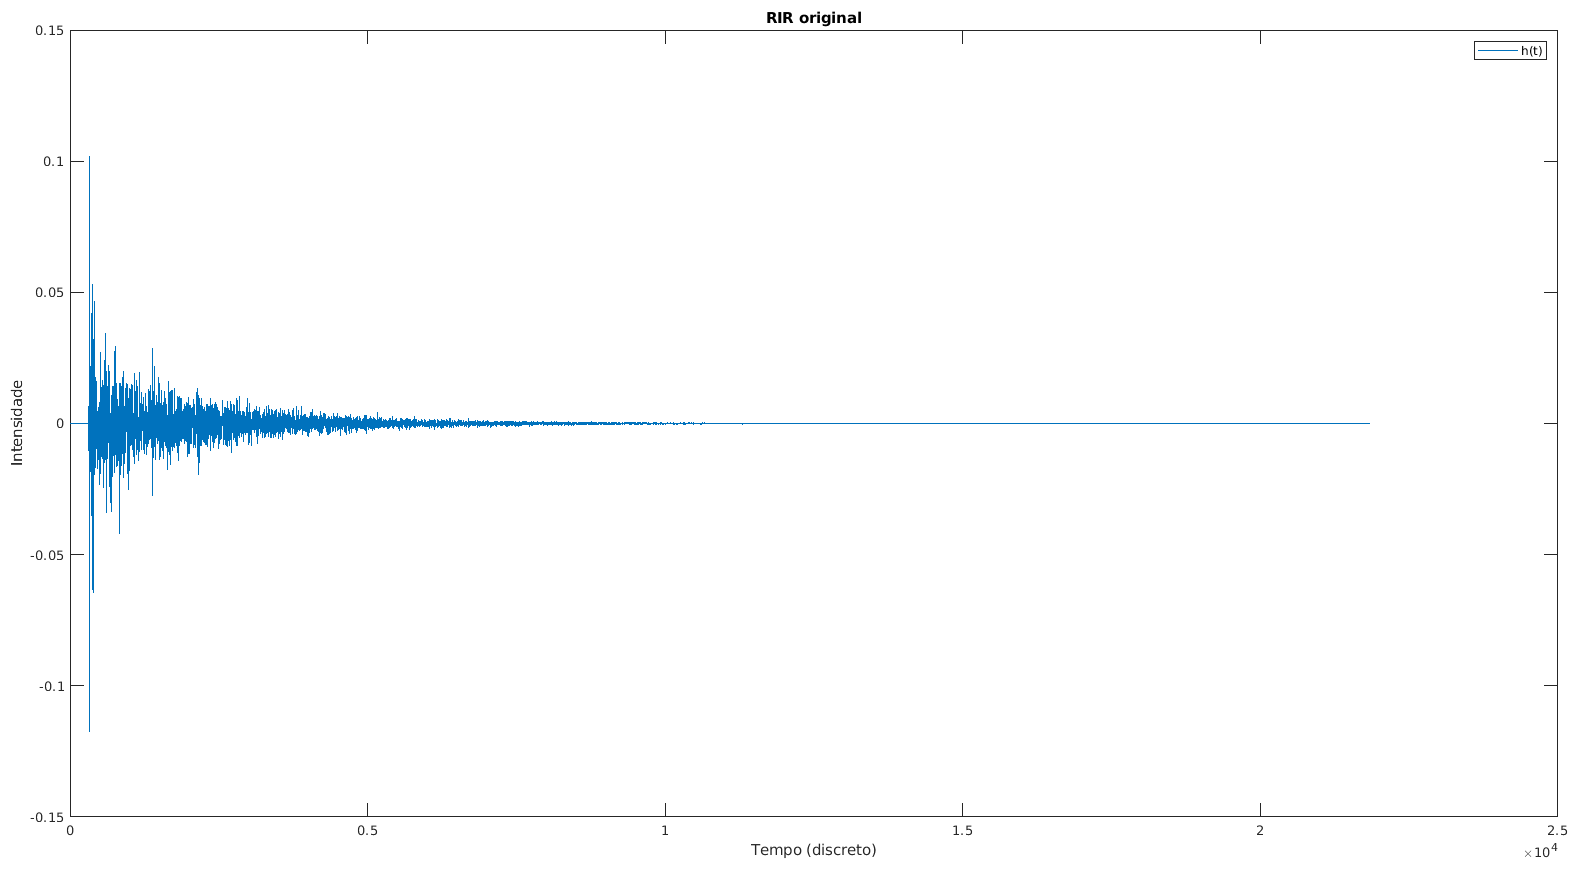
\includegraphics[scale=0.25]{rir-og-n1.png}
    \caption{RIR original.}
    \label{fig-a:rir-og-n1}
\end{figure} 

\begin{figure} [H]
    \centering
    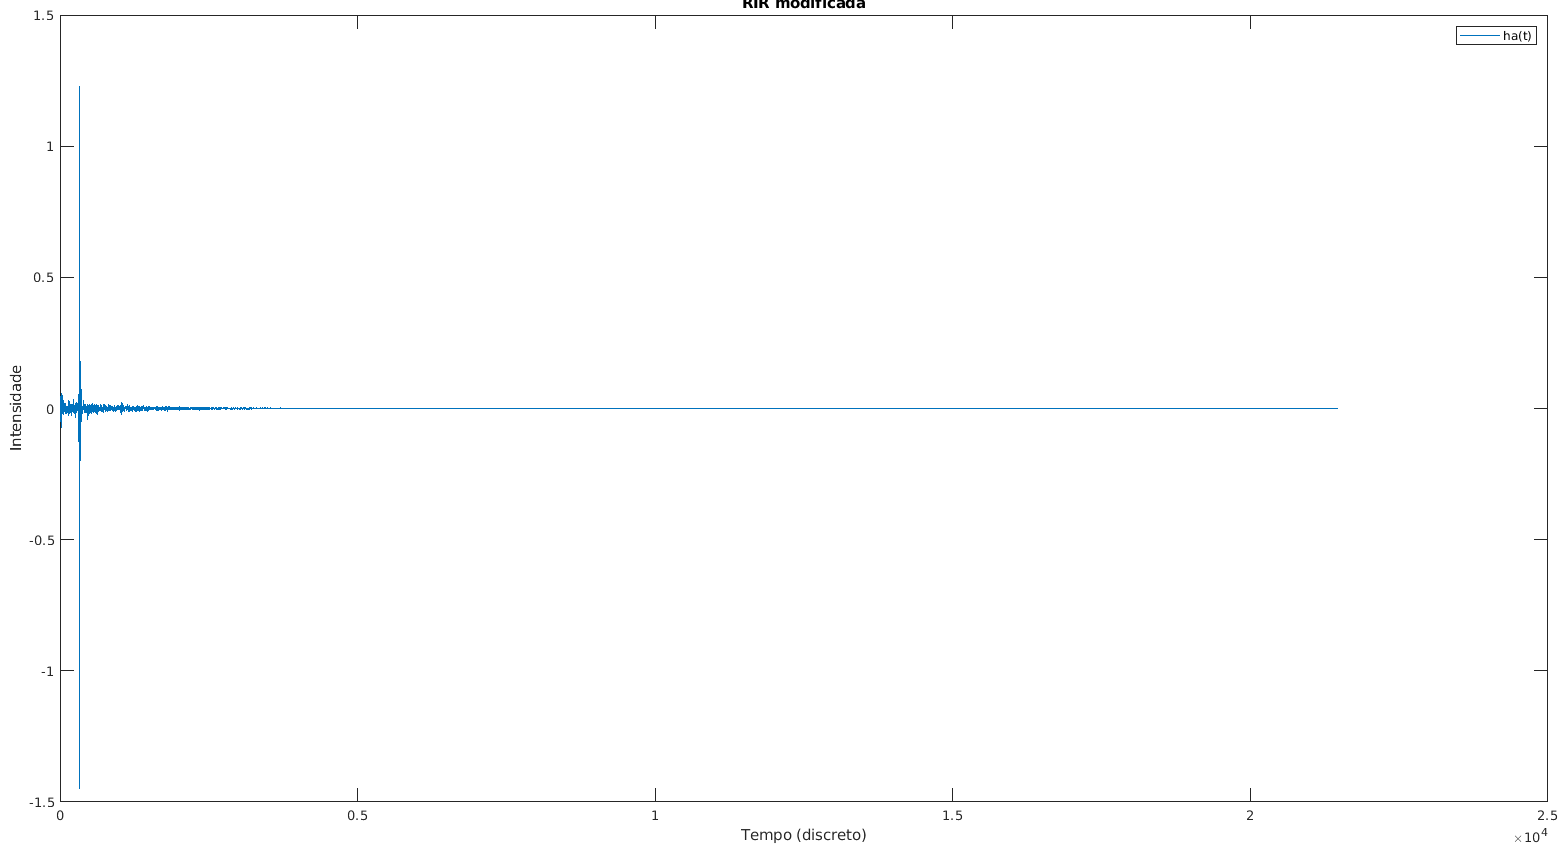
\includegraphics[scale=0.25]{rir-aug-n1.png}
    \caption{RIR simulada.}
    \label{fig-a:rir-aug-n1}
\end{figure} 

\begin{figure} [H]
    \centering
    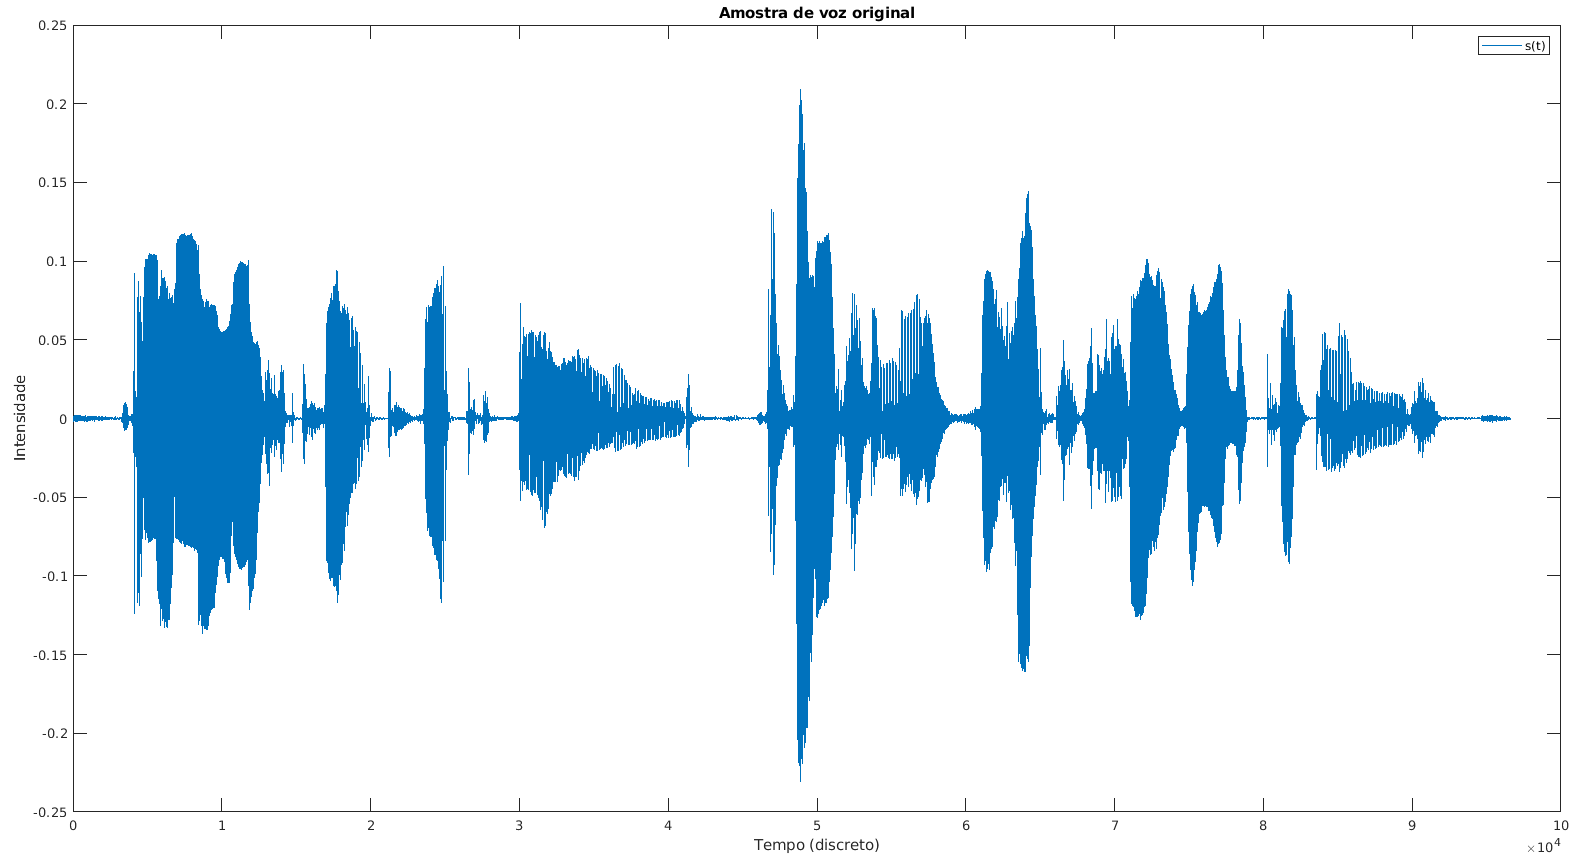
\includegraphics[scale=0.25]{voice-og-n1.png}
    \caption{Amostra de voz original.}
    \label{fig-a:voice-og-n1}
\end{figure} 

\begin{figure} [H]
    \centering
    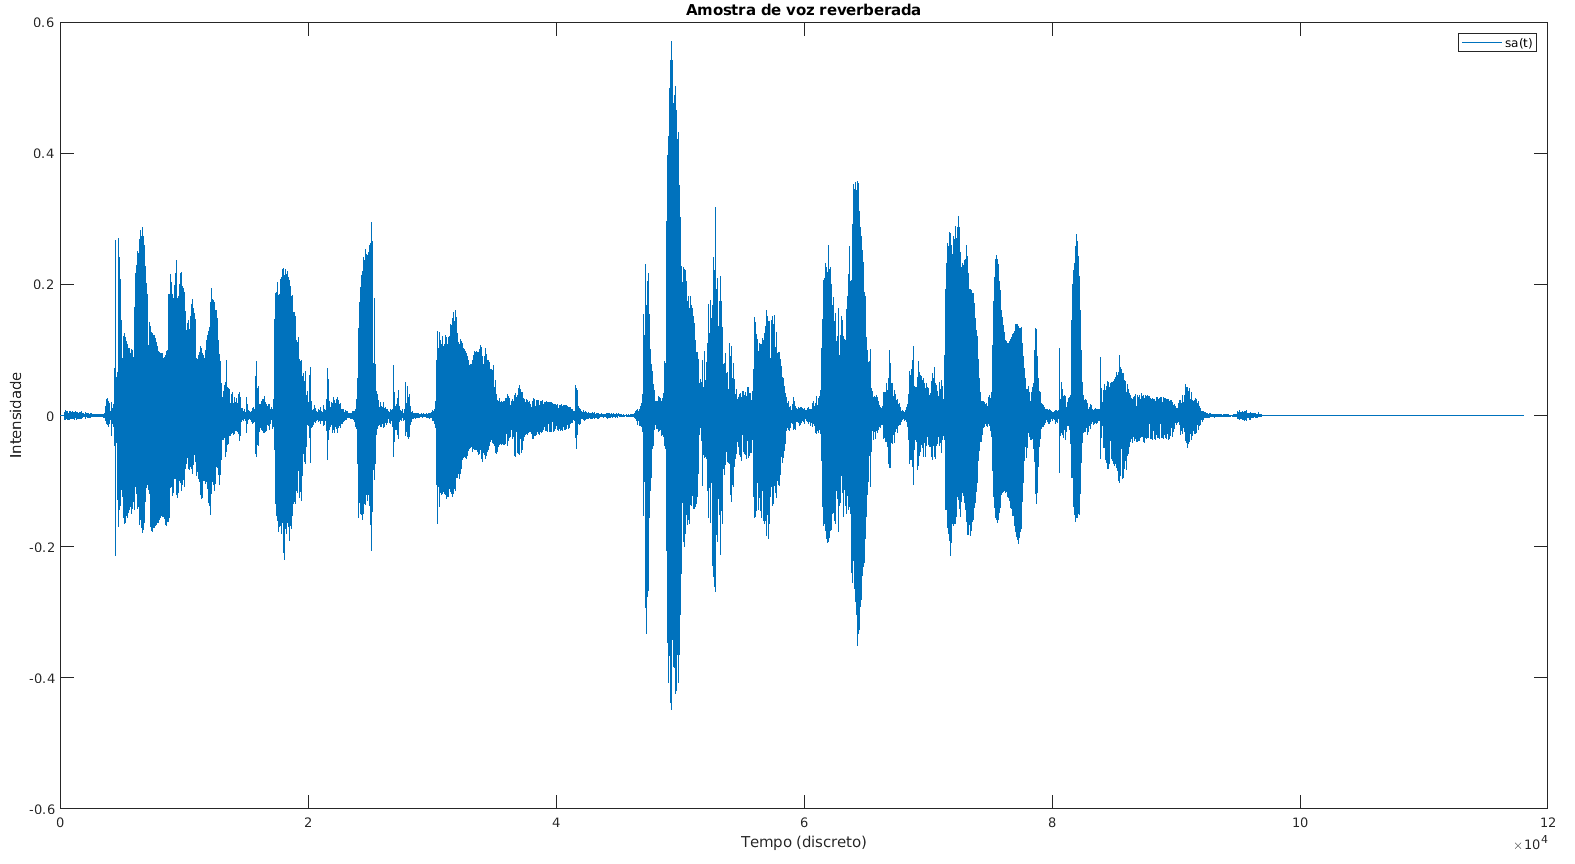
\includegraphics[scale=0.25]{voice-aug-n1.png}
    \caption{Amostra de voz reverberada com RIRSM.}
    \label{fig-a:voice-aug-n1}
\end{figure}

\begin{figure} [H]
    \centering
    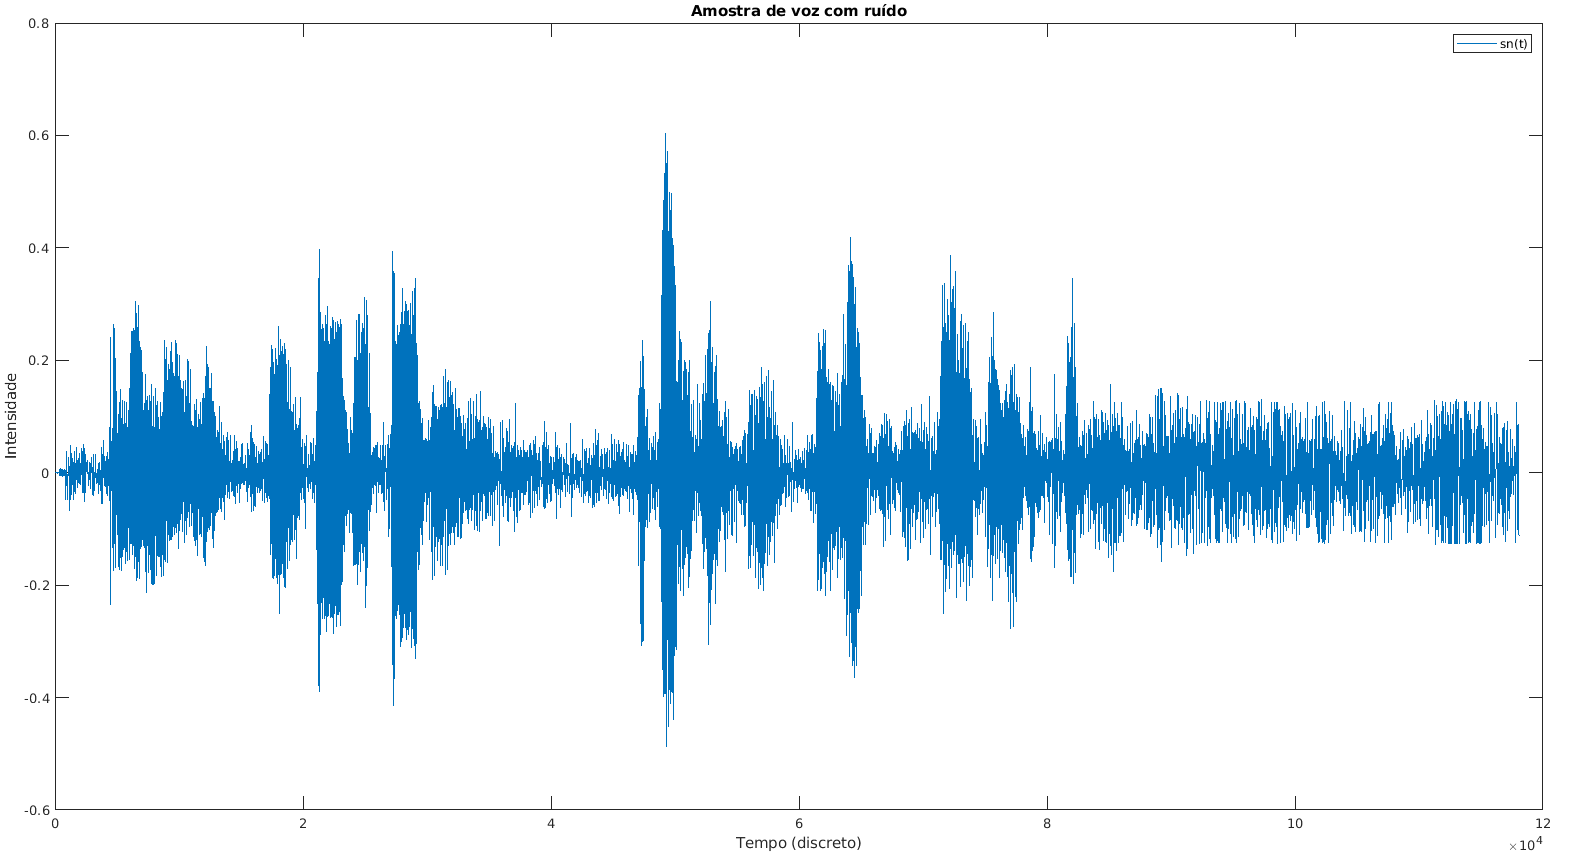
\includegraphics[scale=0.25]{voice-ns-n1.png}
    \caption{Amostra de voz em campo distante.}
    \label{fig-a:voice-ns-n1}
\end{figure}

\pagebreak
{\Large \textbf{Exemplo N2}}

\begin{figure} [H]
    \centering
    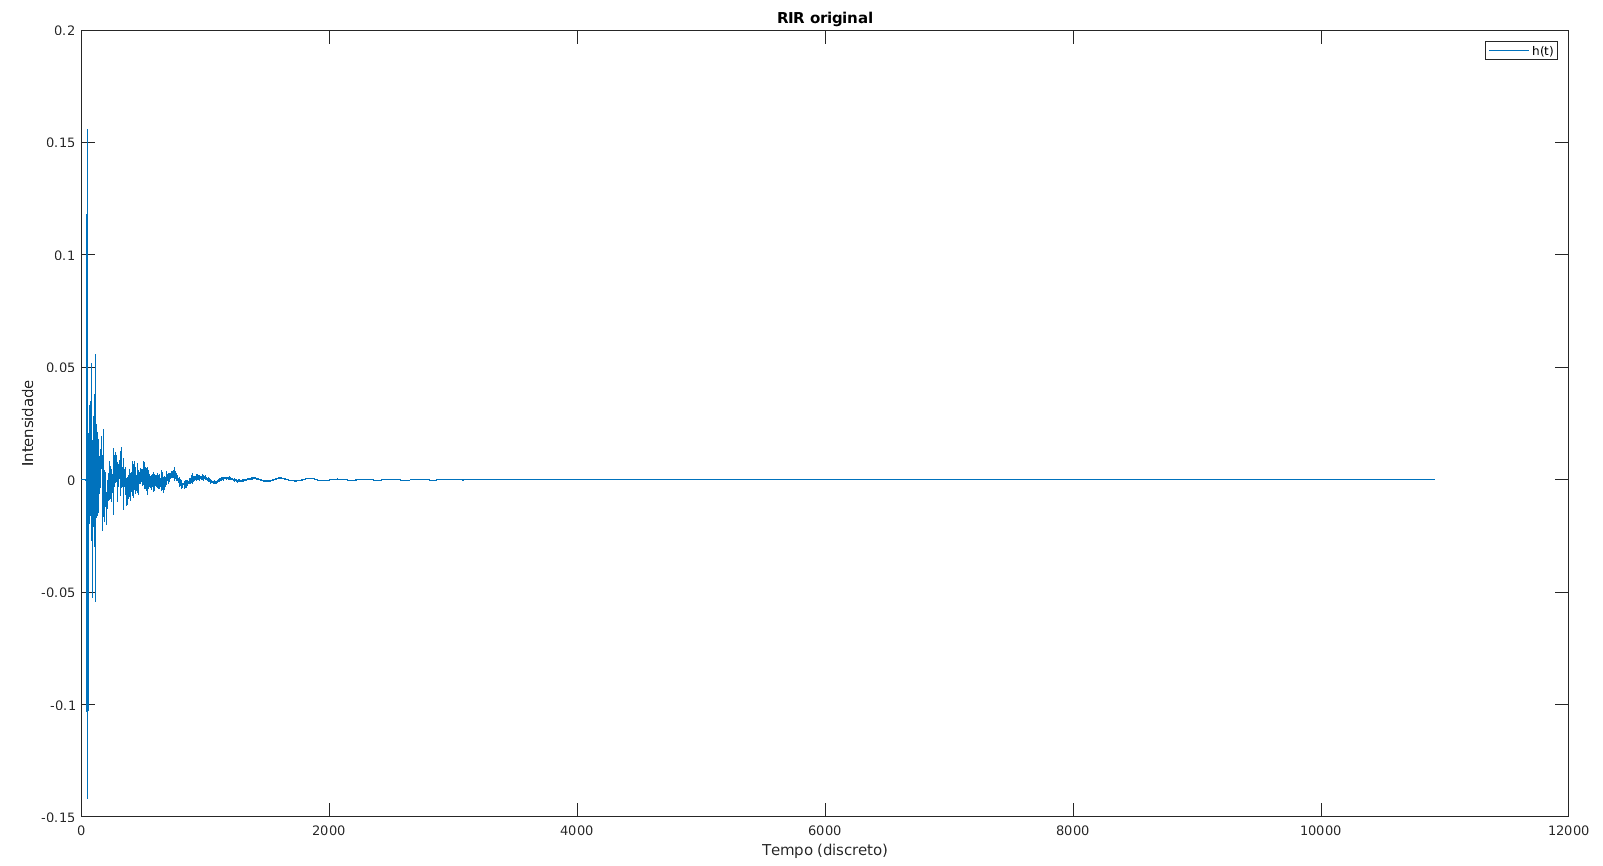
\includegraphics[scale=0.25]{rir-og-n2.png}
    \caption{RIR original.}
    \label{fig-a:rir-og-n2}
\end{figure} 

\begin{figure} [H]
    \centering
    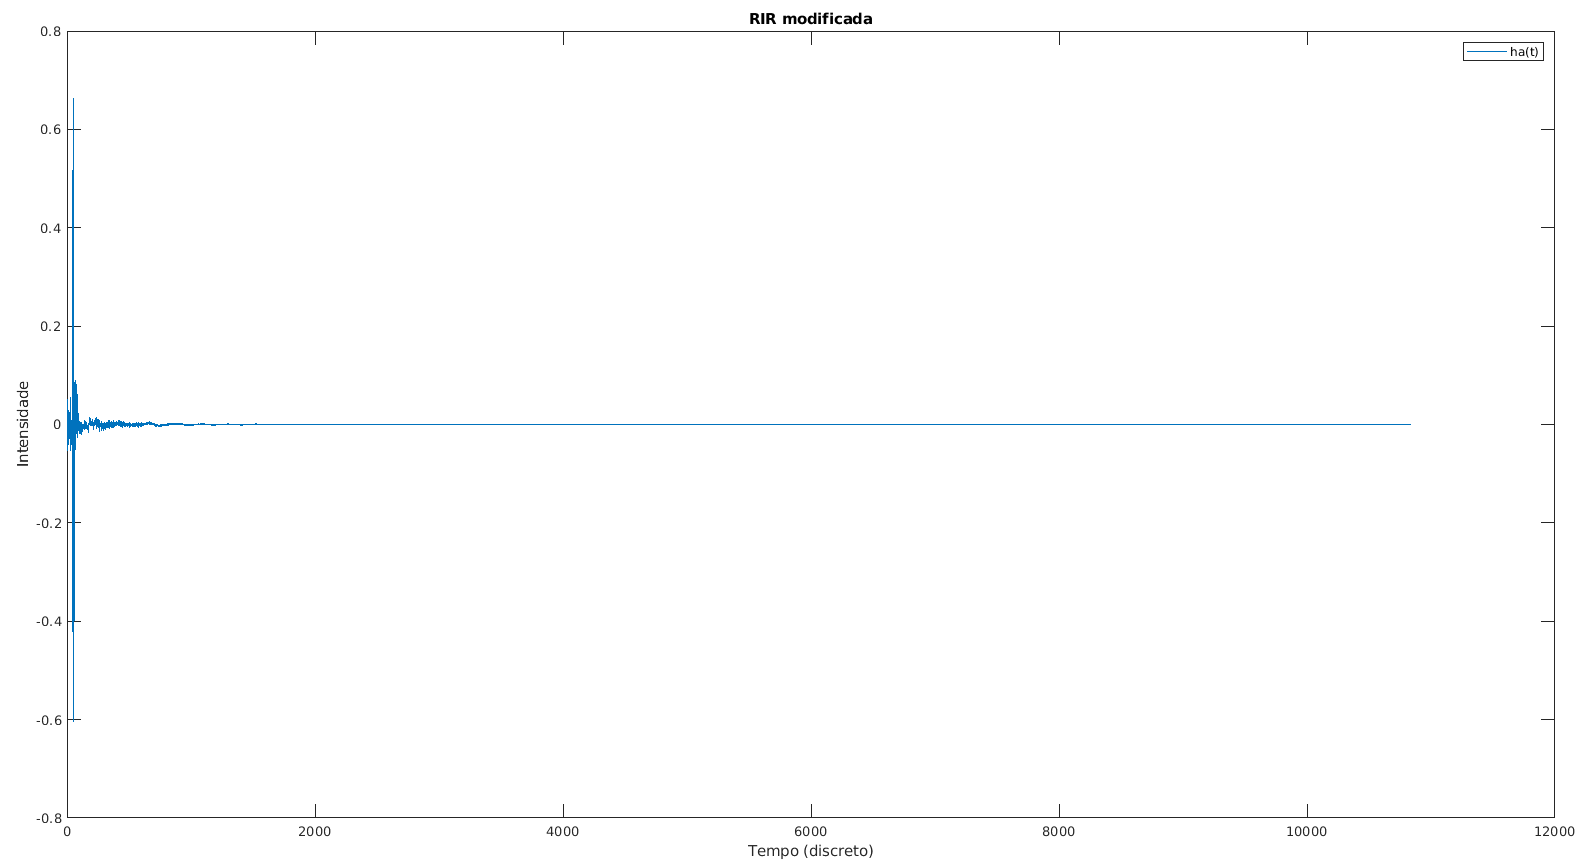
\includegraphics[scale=0.25]{rir-aug-n2.png}
    \caption{RIR simulada.}
    \label{fig-a:rir-aug-n2}
\end{figure} 

\begin{figure} [H]
    \centering
    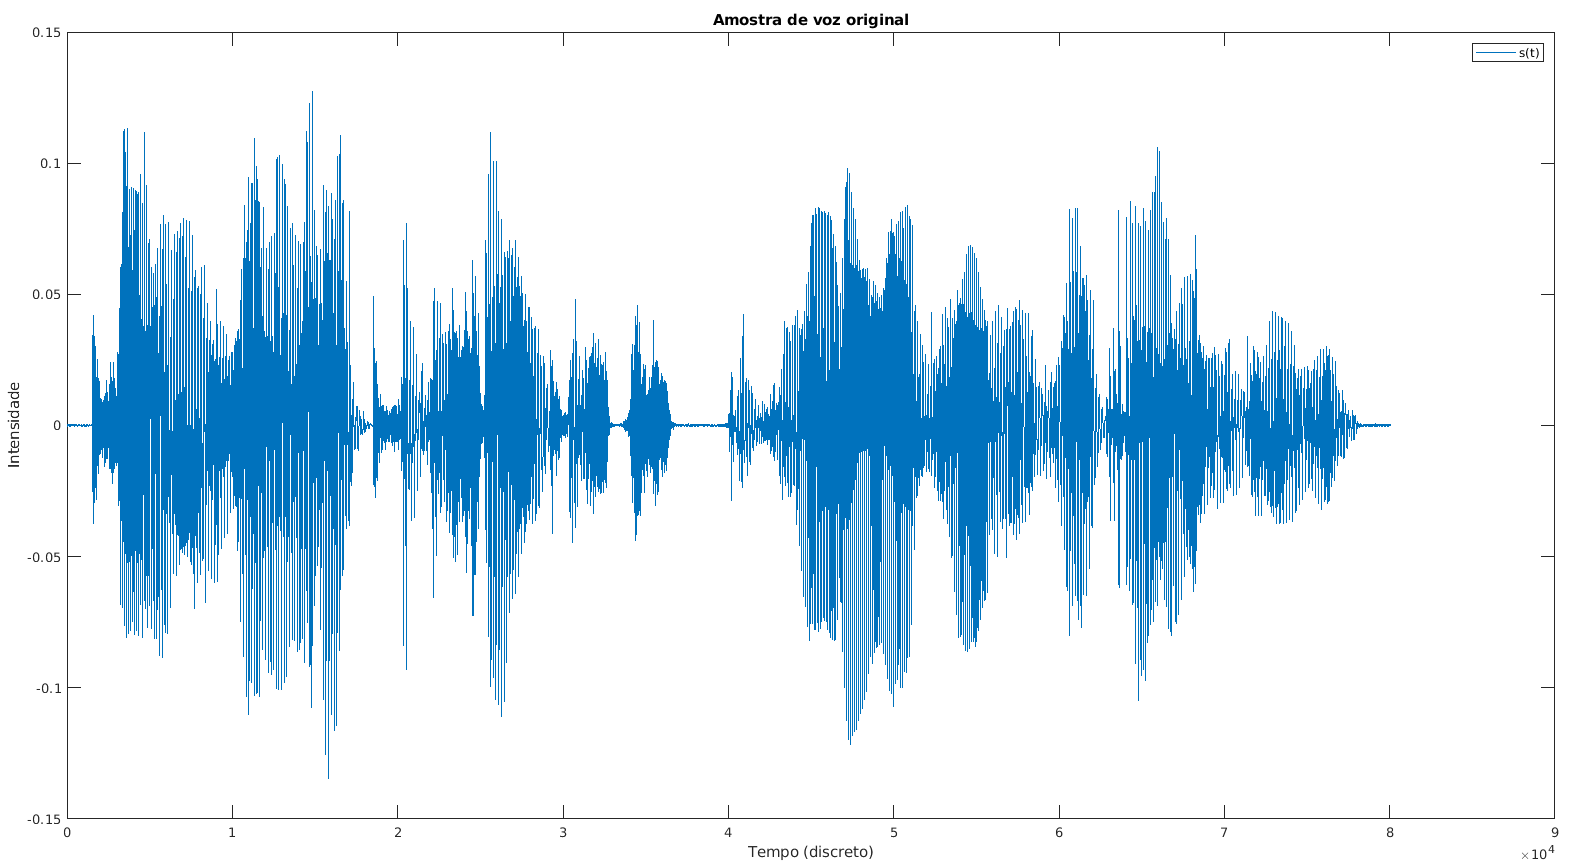
\includegraphics[scale=0.25]{voice-og-n2.png}
    \caption{Amostra de voz original.}
    \label{fig-a:voice-og-n2}
\end{figure} 

\begin{figure} [H]
    \centering
    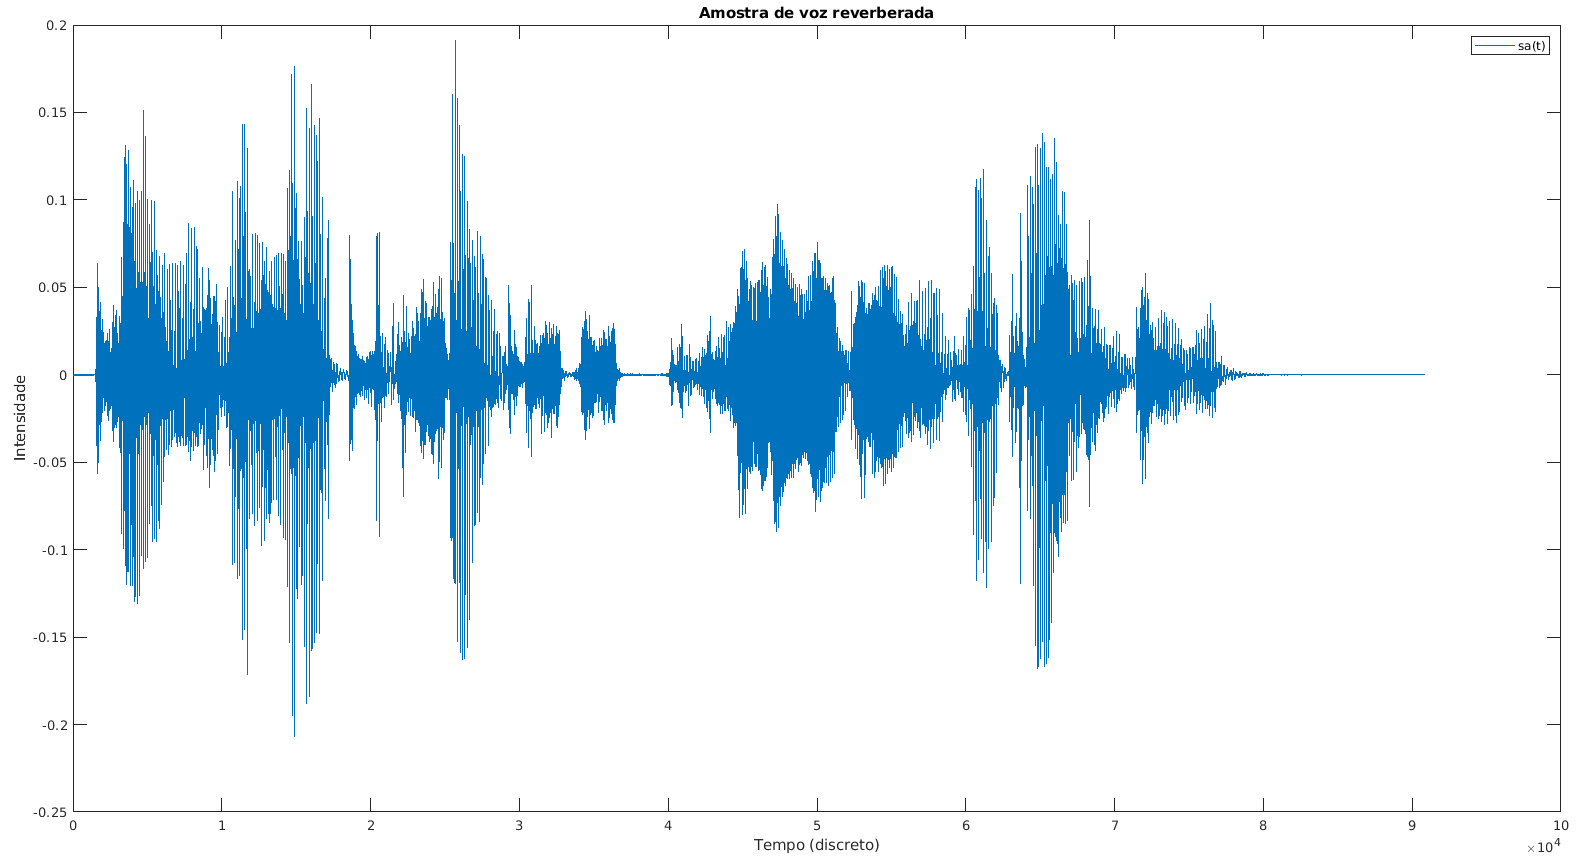
\includegraphics[scale=0.25]{voice-aug-n2.png}
    \caption{Amostra de voz reverberada com RIRSM.}
    \label{fig-a:voice-aug-n2}
\end{figure}

\begin{figure} [H]
    \centering
    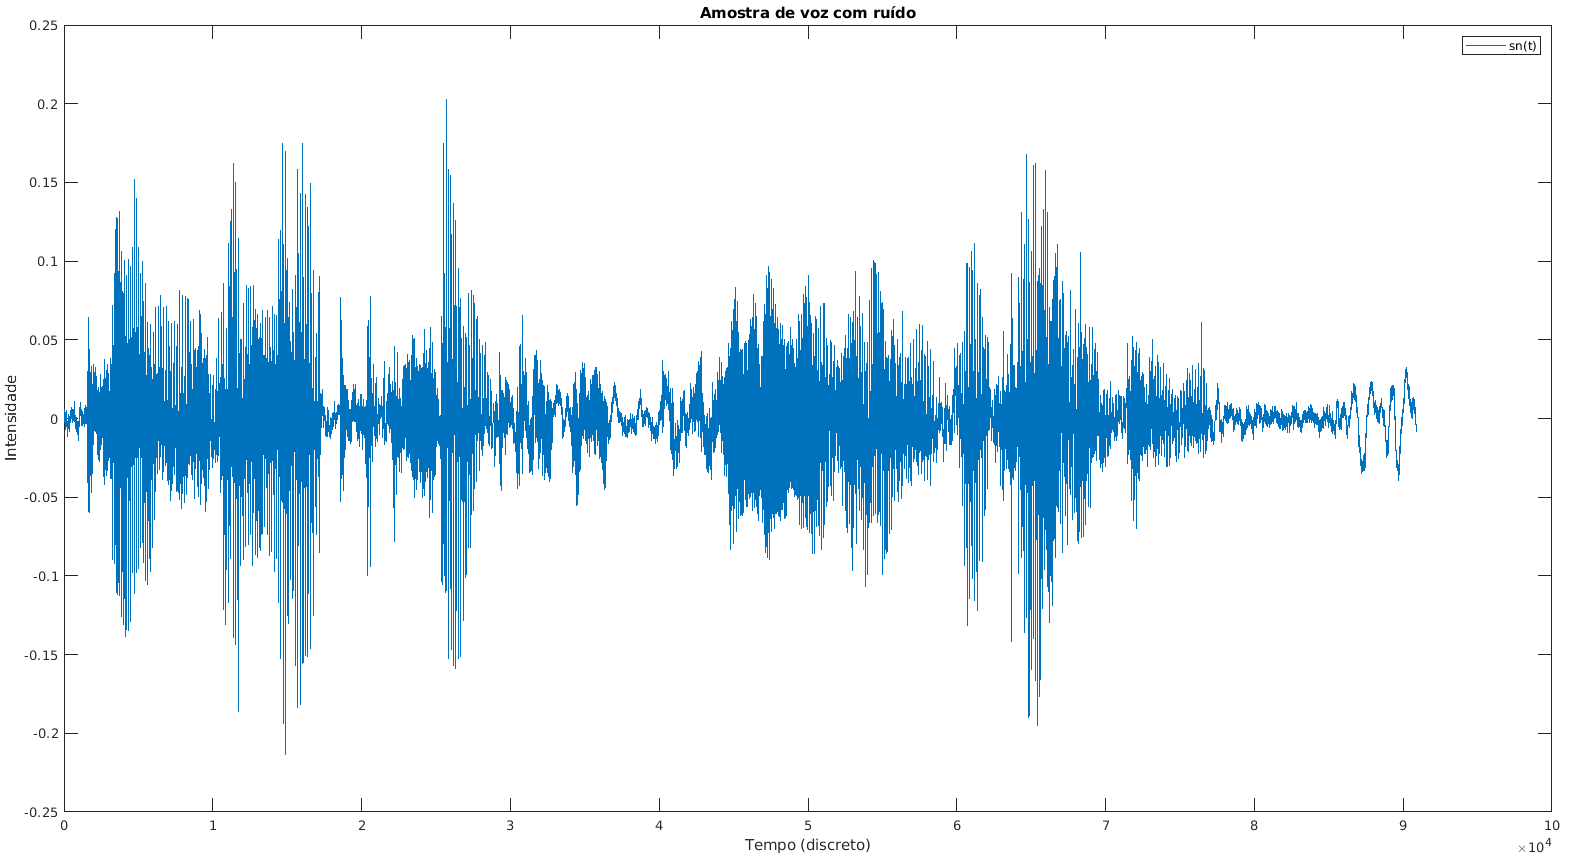
\includegraphics[scale=0.25]{voice-ns-n2.png}
    \caption{Amostra de voz em campo distante.}
    \label{fig-a:voice-ns-n2}
\end{figure}

\pagebreak
{\Large \textbf{Exemplo N3}}

\begin{figure} [H]
    \centering
    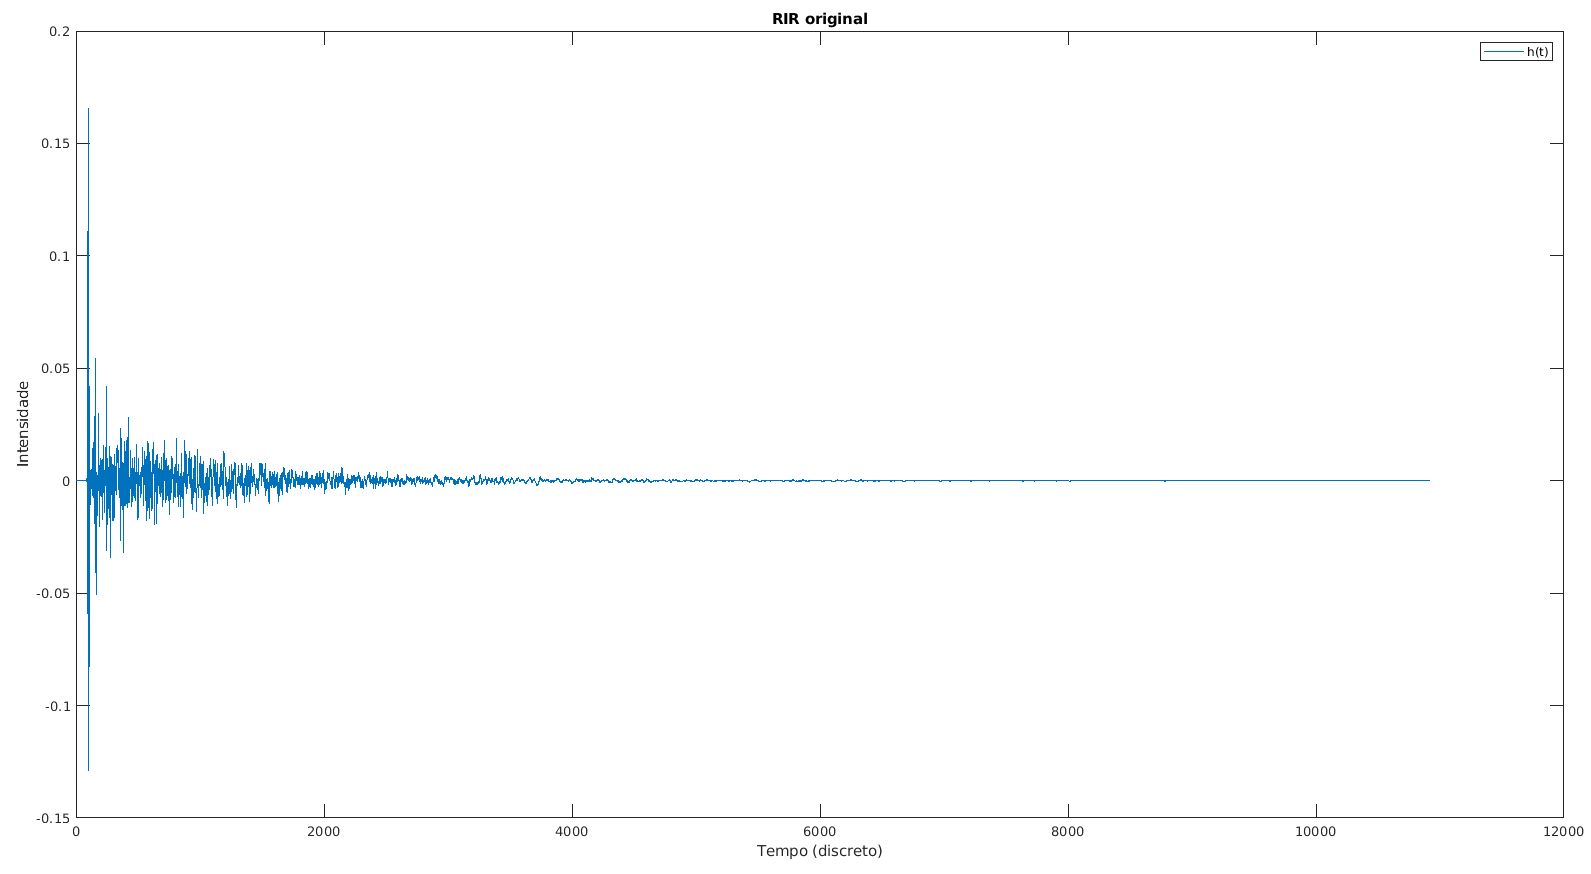
\includegraphics[scale=0.25]{rir-og-n3.png}
    \caption{RIR original.}
    \label{fig-a:rir-og-n3}
\end{figure} 

\begin{figure} [H]
    \centering
    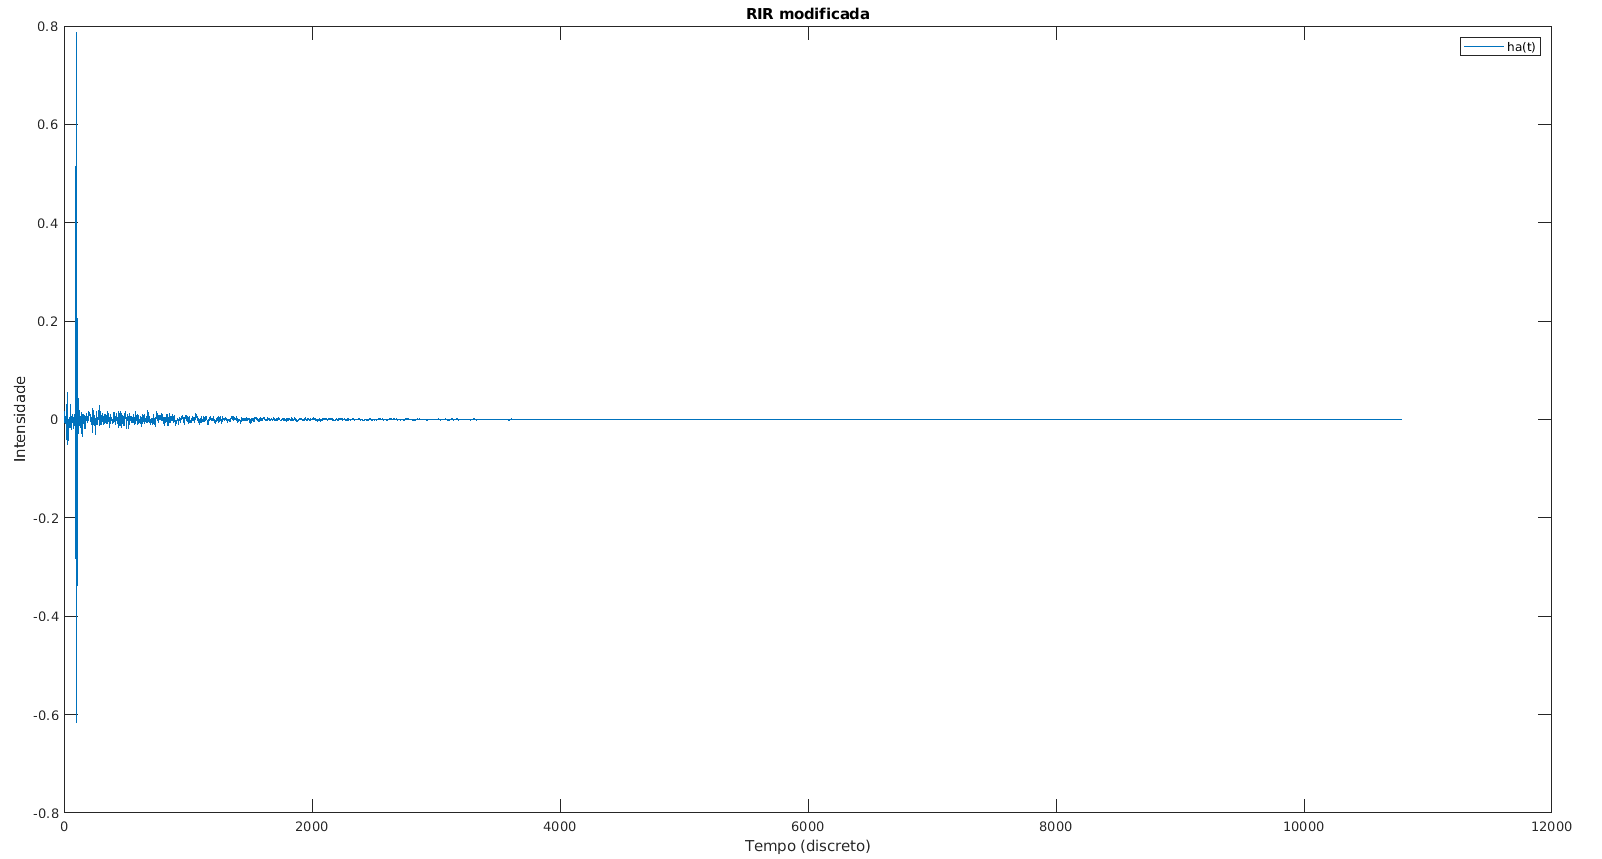
\includegraphics[scale=0.25]{rir-aug-n3.png}
    \caption{RIR simulada.}
    \label{fig-a:rir-aug-n3}
\end{figure} 

\begin{figure} [H]
    \centering
    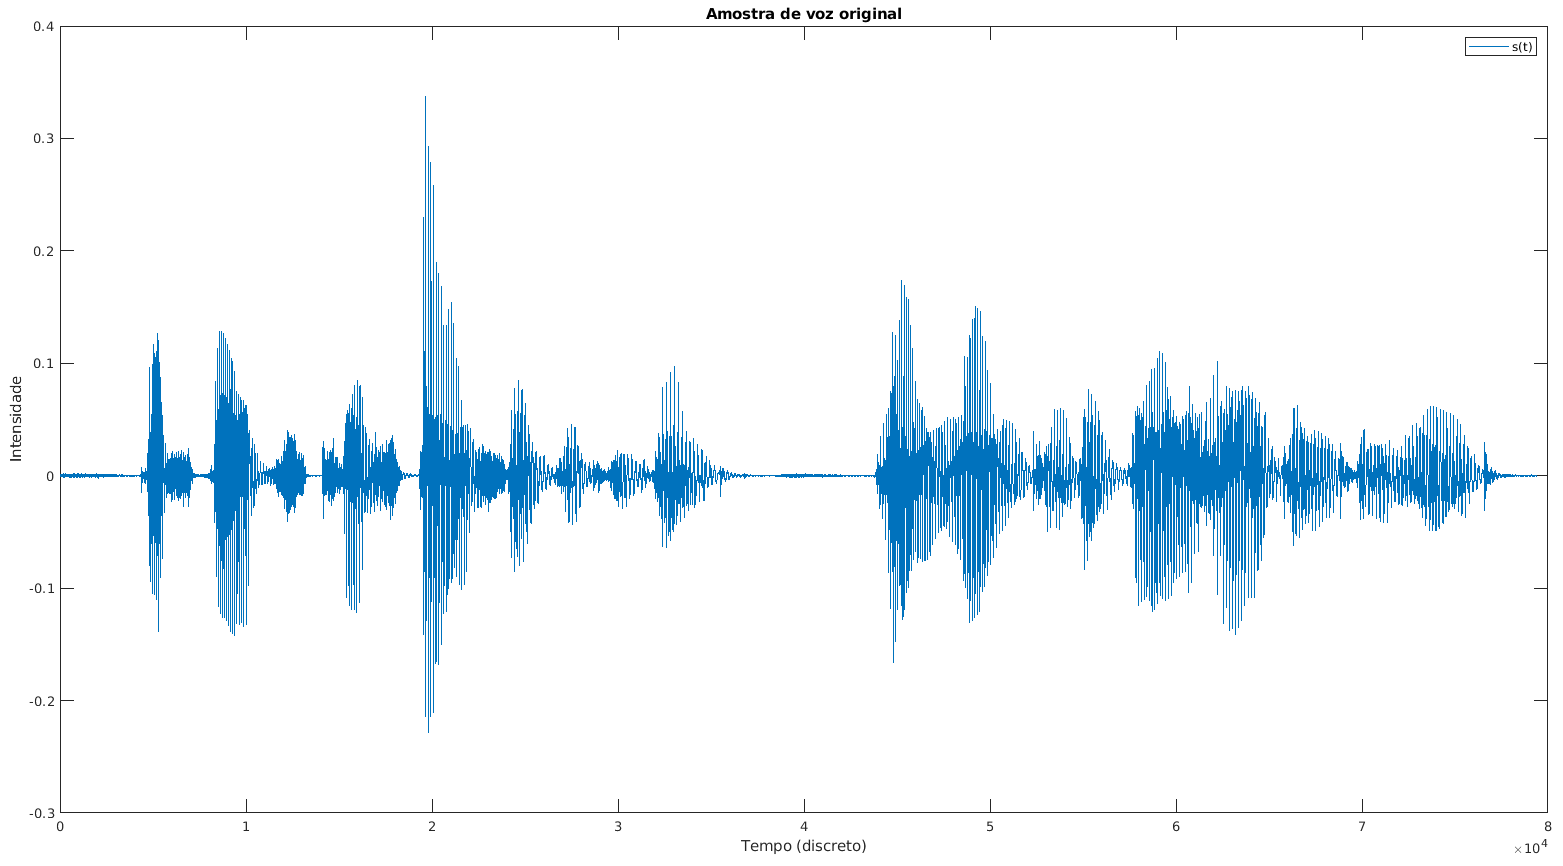
\includegraphics[scale=0.25]{voice-og-n3.png}
    \caption{Amostra de voz original.}
    \label{fig-a:voice-og-n3}
\end{figure} 

\begin{figure} [H]
    \centering
    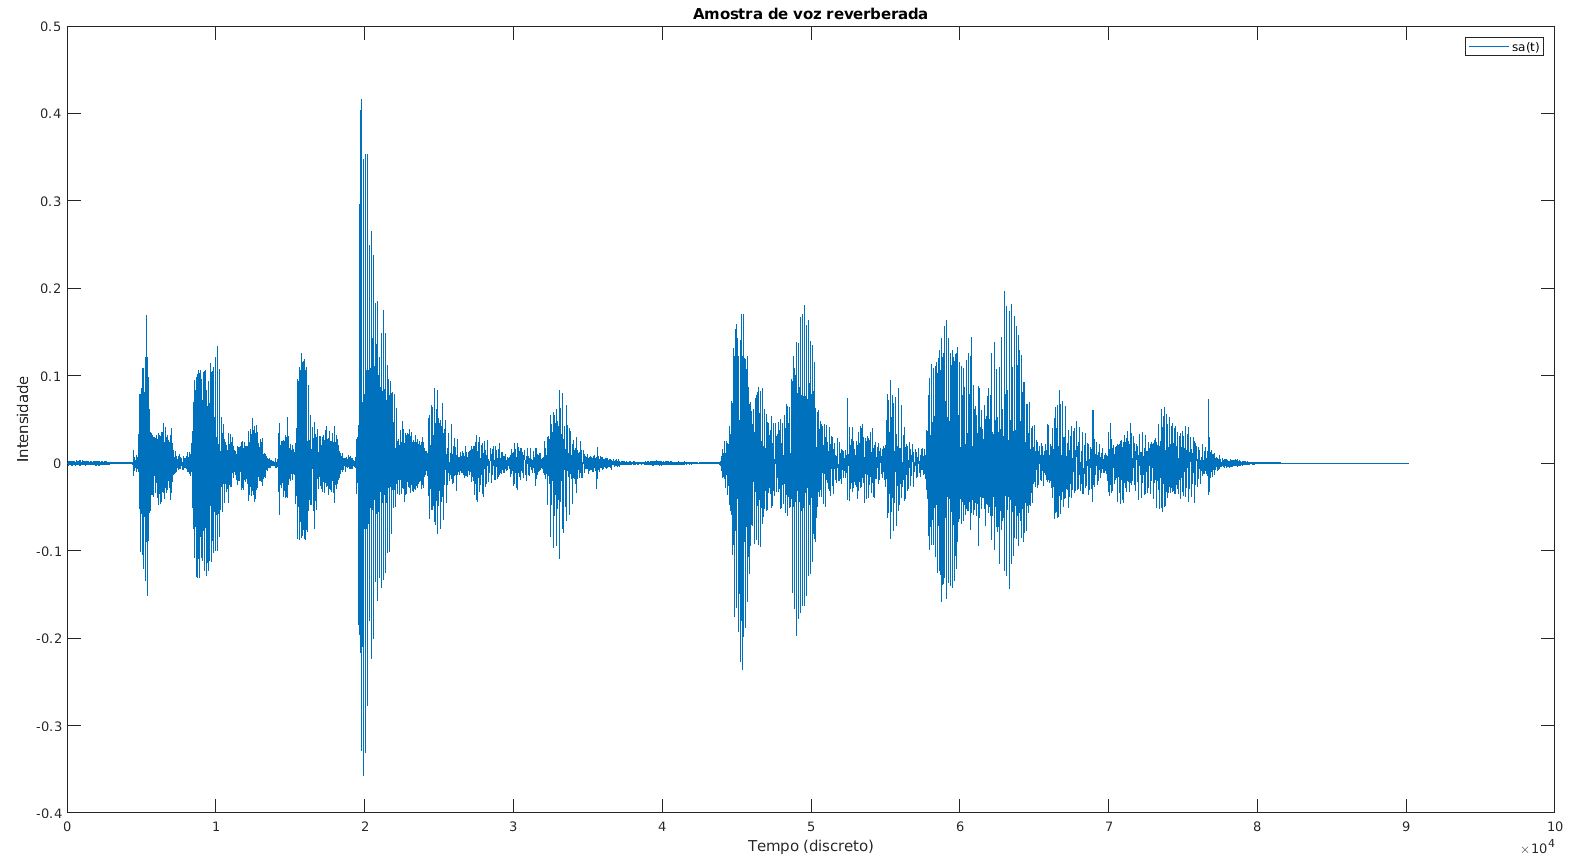
\includegraphics[scale=0.25]{voice-aug-n3.png}
    \caption{Amostra de voz reverberada com RIRSM.}
    \label{fig-a:voice-aug-n3}
\end{figure}

\begin{figure} [H]
    \centering
    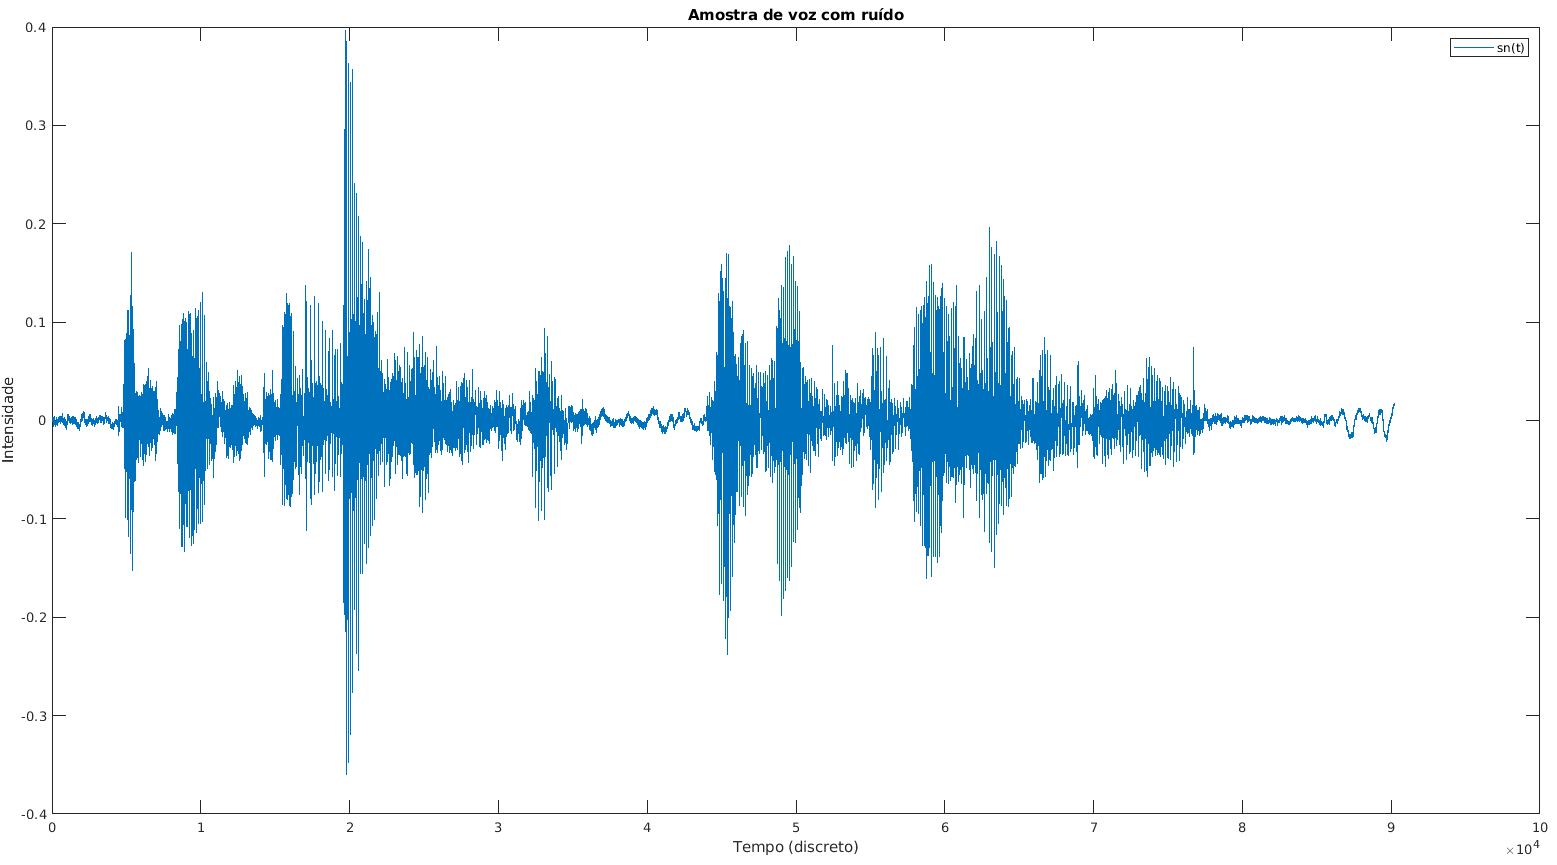
\includegraphics[scale=0.25]{voice-ns-n3.png}
    \caption{Amostra de voz em campo distante.}
    \label{fig-a:voice-ns-n3}
\end{figure}

\pagebreak
{\Large \textbf{Exemplo N4}}

\begin{figure} [H]
    \centering
    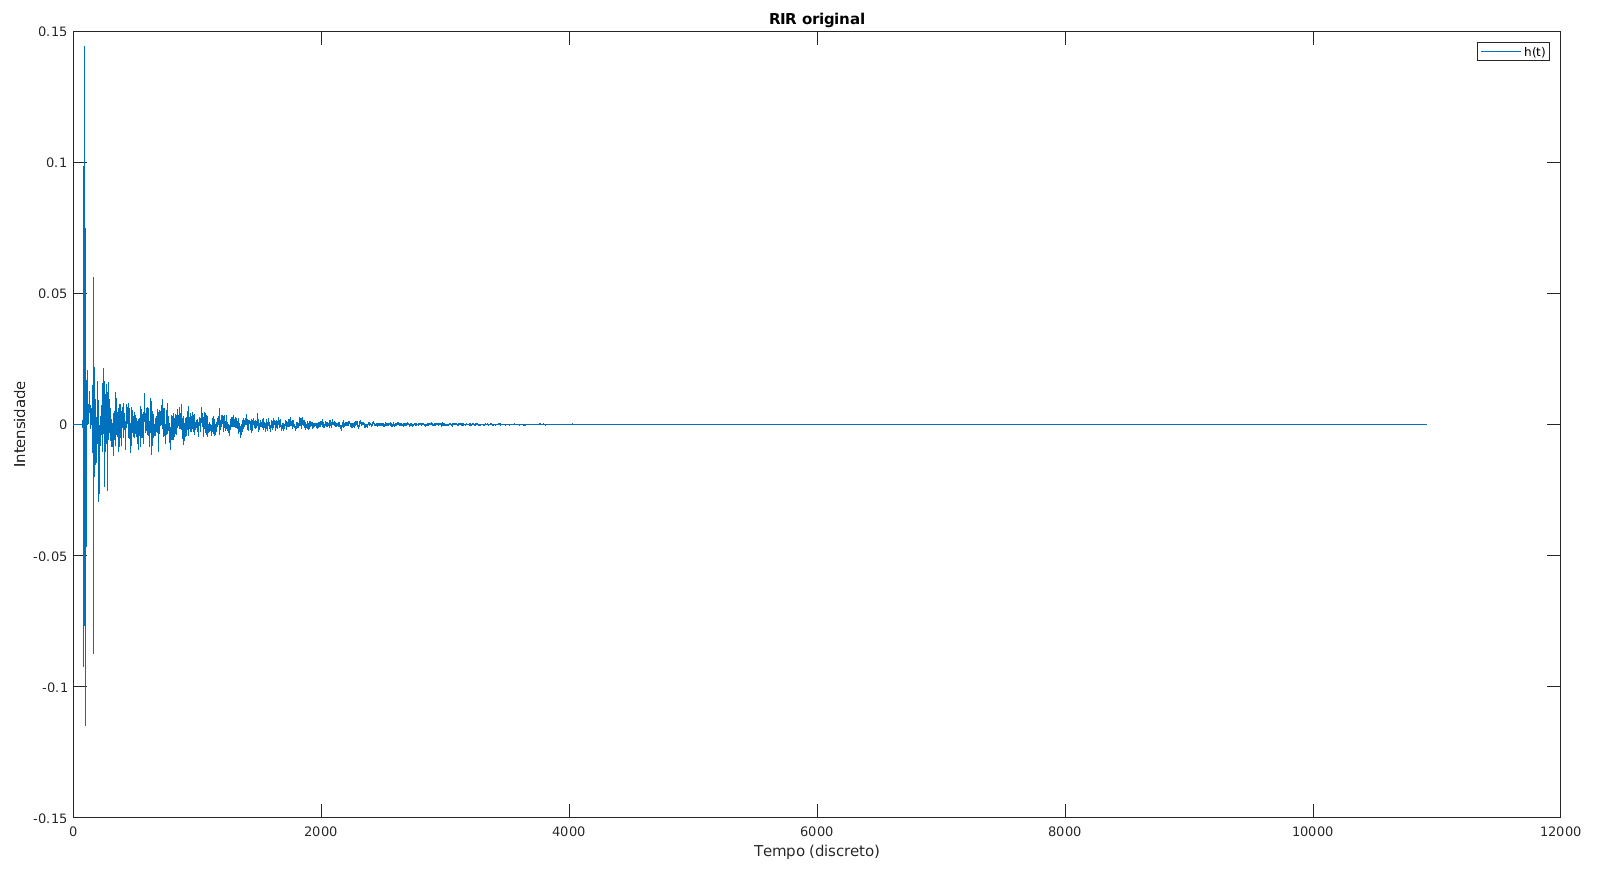
\includegraphics[scale=0.25]{rir-og-n4.png}
    \caption{RIR original.}
    \label{fig-a:rir-og-n4}
\end{figure} 

\begin{figure} [H]
    \centering
    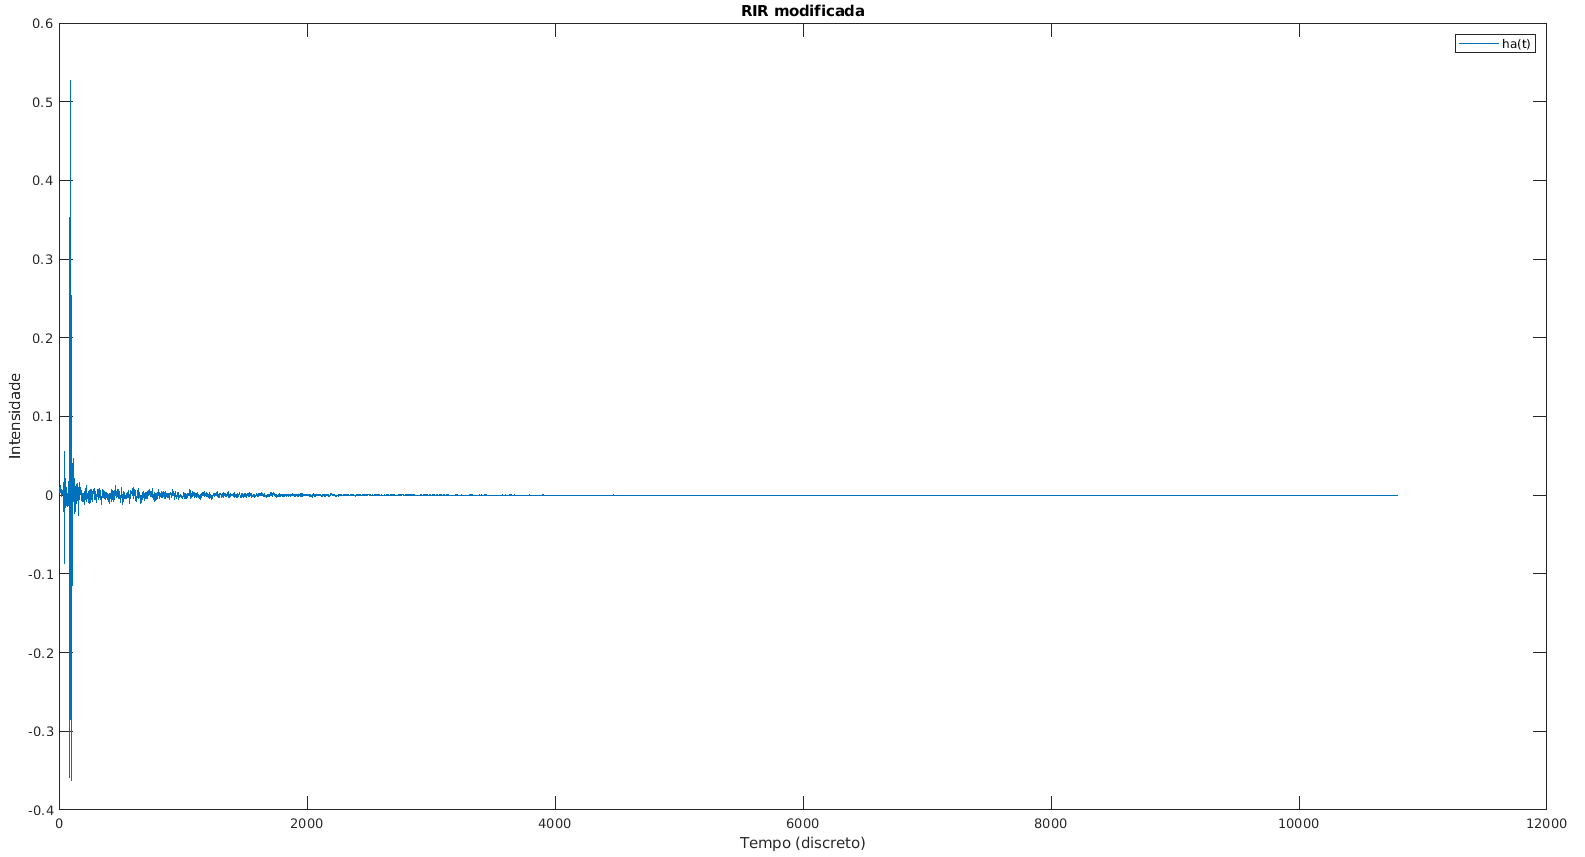
\includegraphics[scale=0.25]{rir-aug-n4.png}
    \caption{RIR simulada.}
    \label{fig-a:rir-aug-n4}
\end{figure} 

\begin{figure} [H]
    \centering
    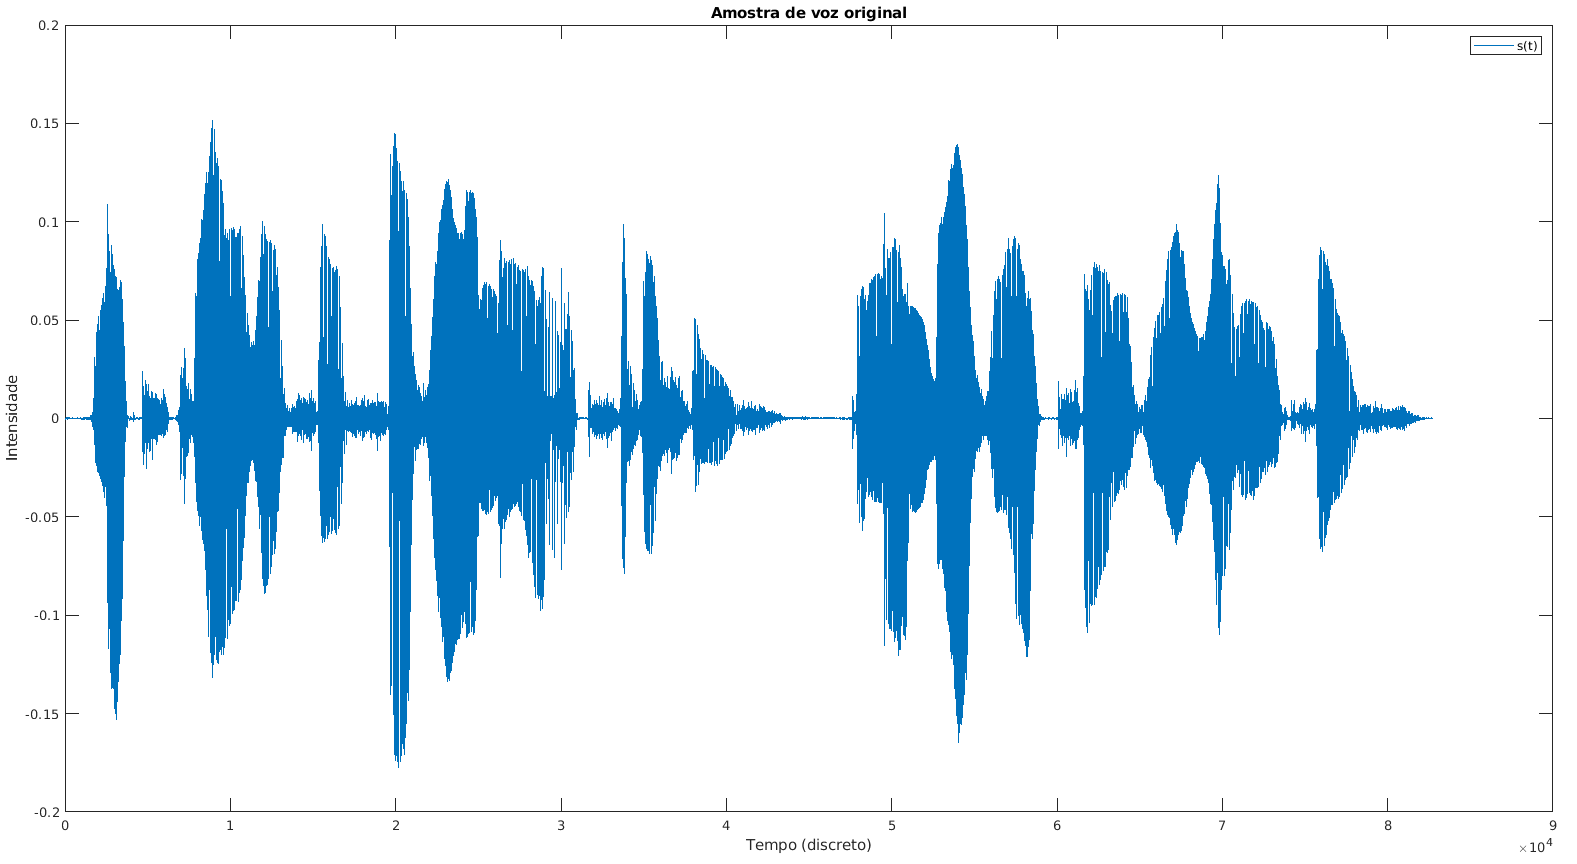
\includegraphics[scale=0.25]{voice-og-n4.png}
    \caption{Amostra de voz original.}
    \label{fig-a:voice-og-n4}
\end{figure} 

\begin{figure} [H]
    \centering
    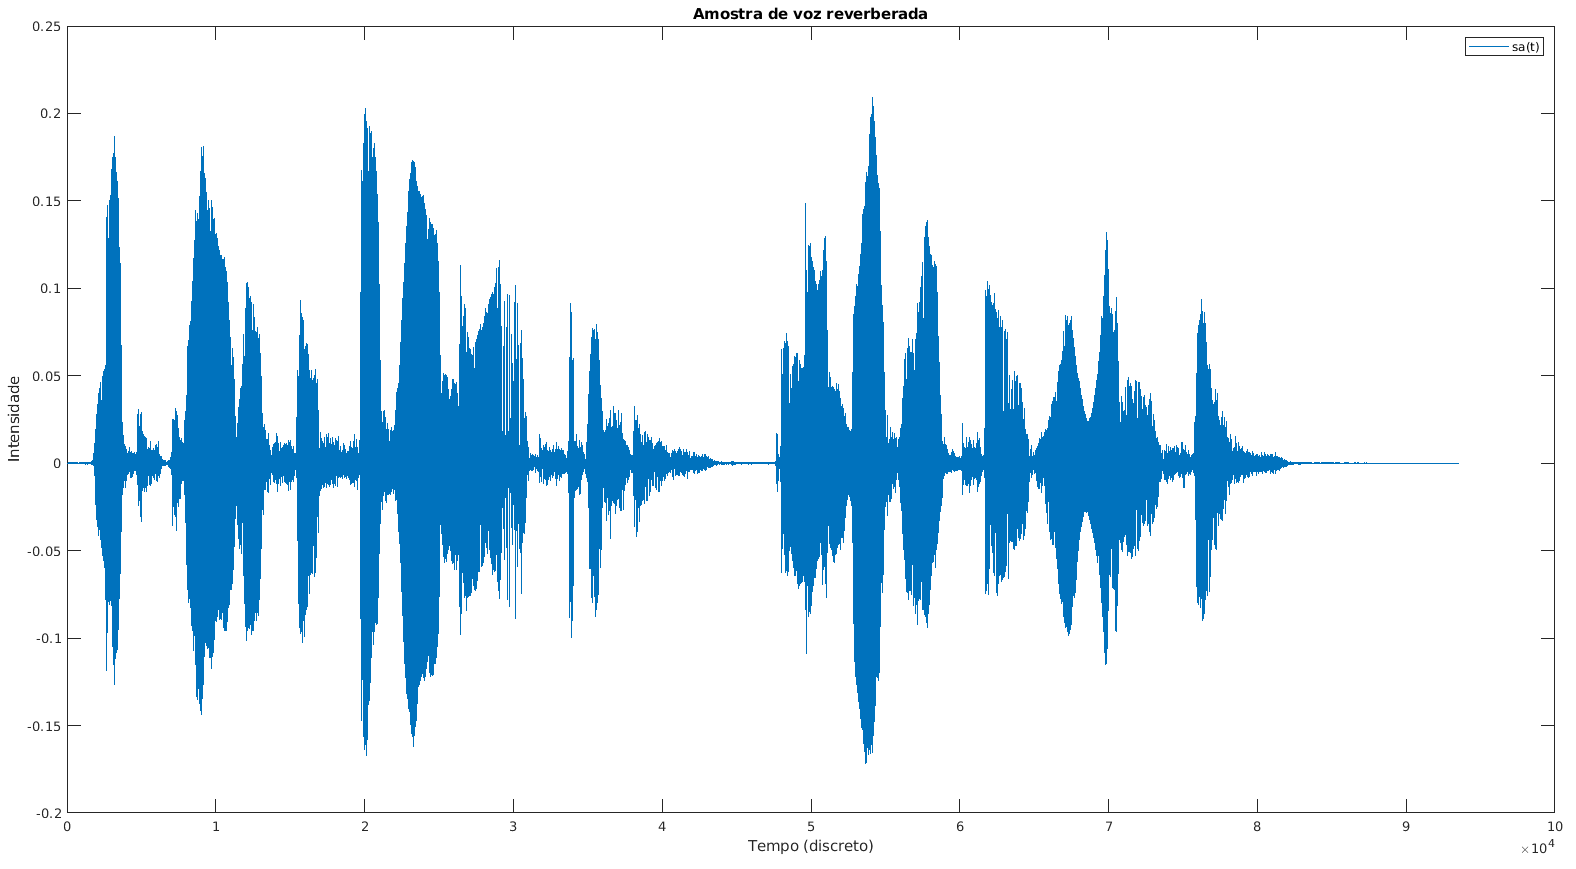
\includegraphics[scale=0.25]{voice-aug-n4.png}
    \caption{Amostra de voz reverberada com RIRSM.}
    \label{fig-a:voice-aug-n4}
\end{figure}

\begin{figure} [H]
    \centering
    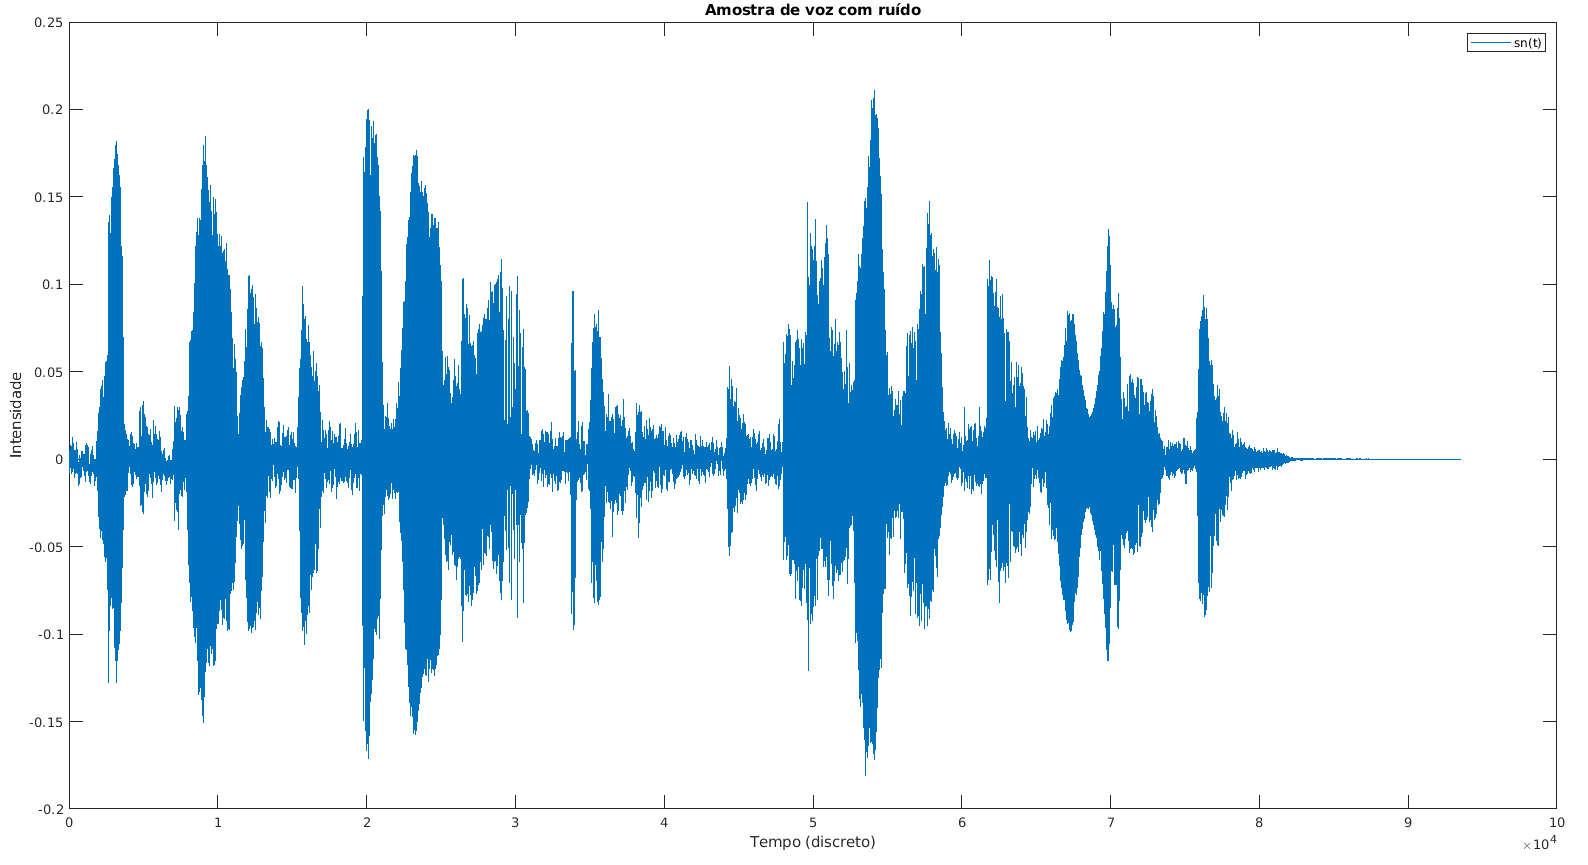
\includegraphics[scale=0.25]{voice-ns-n4.png}
    \caption{Amostra de voz em campo distante.}
    \label{fig-a:voice-ns-n4}
\end{figure}

\pagebreak
{\Large \textbf{Exemplo N5}}

\begin{figure} [H]
    \centering
    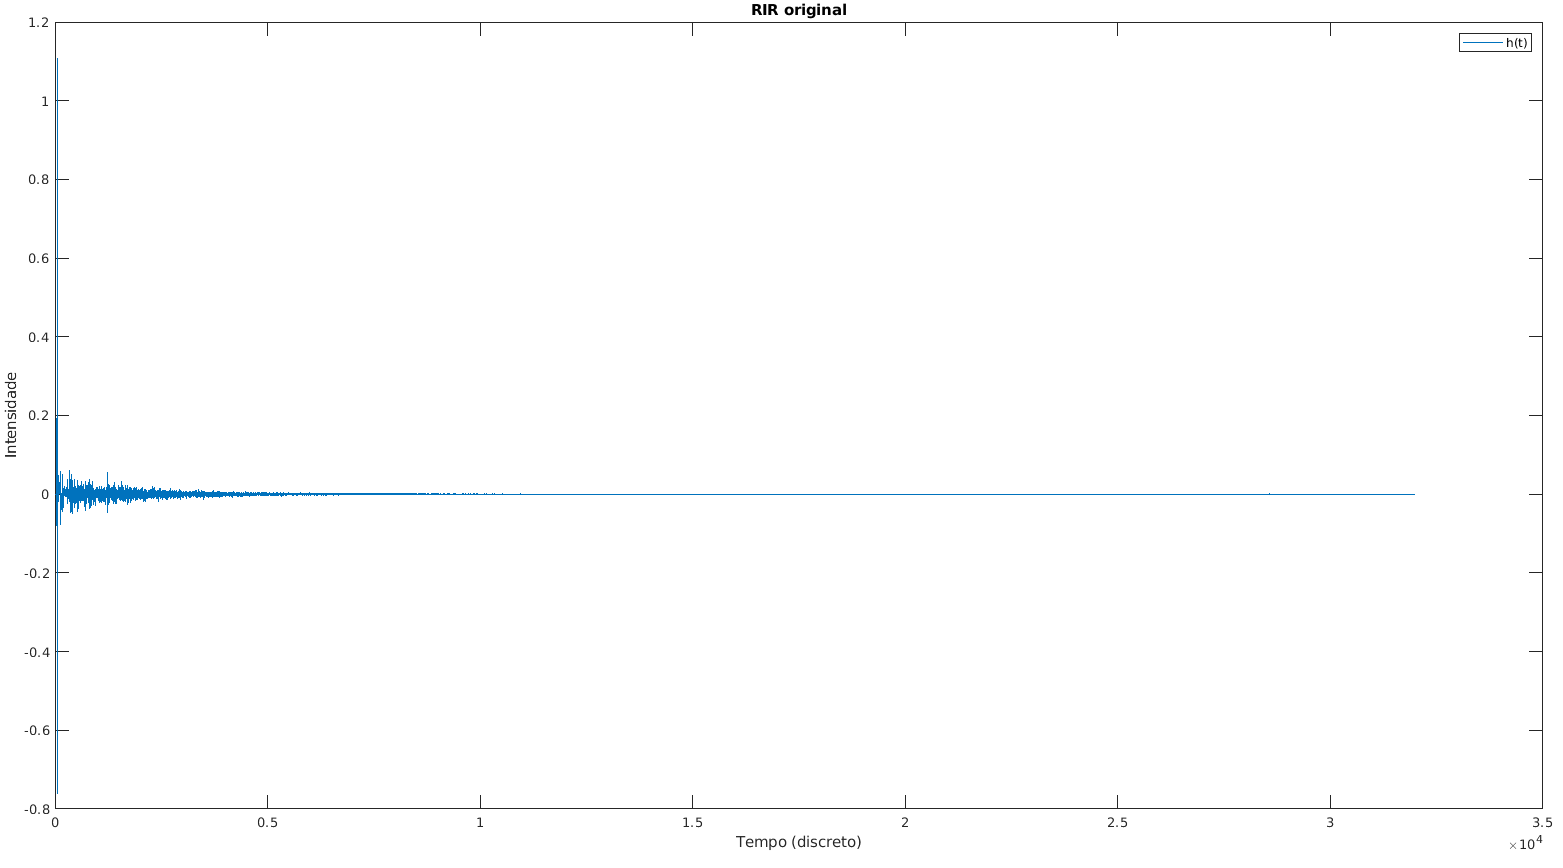
\includegraphics[scale=0.25]{rir-og-n5.png}
    \caption{RIR original.}
    \label{fig-a:rir-og-n5}
\end{figure} 

\begin{figure} [H]
    \centering
    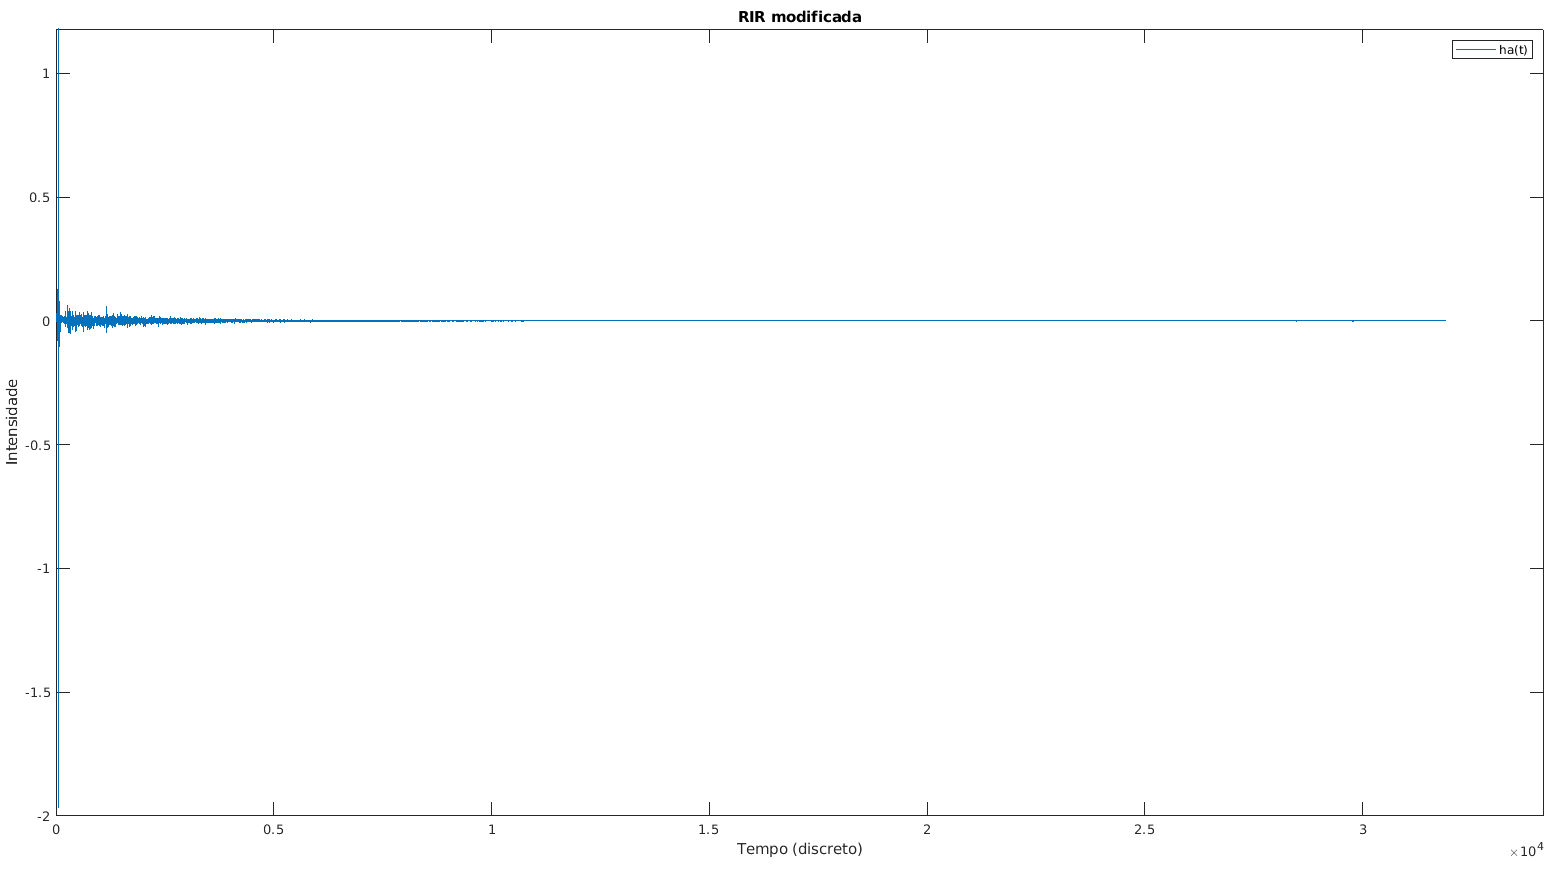
\includegraphics[scale=0.25]{rir-aug-n5.png}
    \caption{RIR simulada.}
    \label{fig-a:rir-aug-n5}
\end{figure} 

\begin{figure} [H]
    \centering
    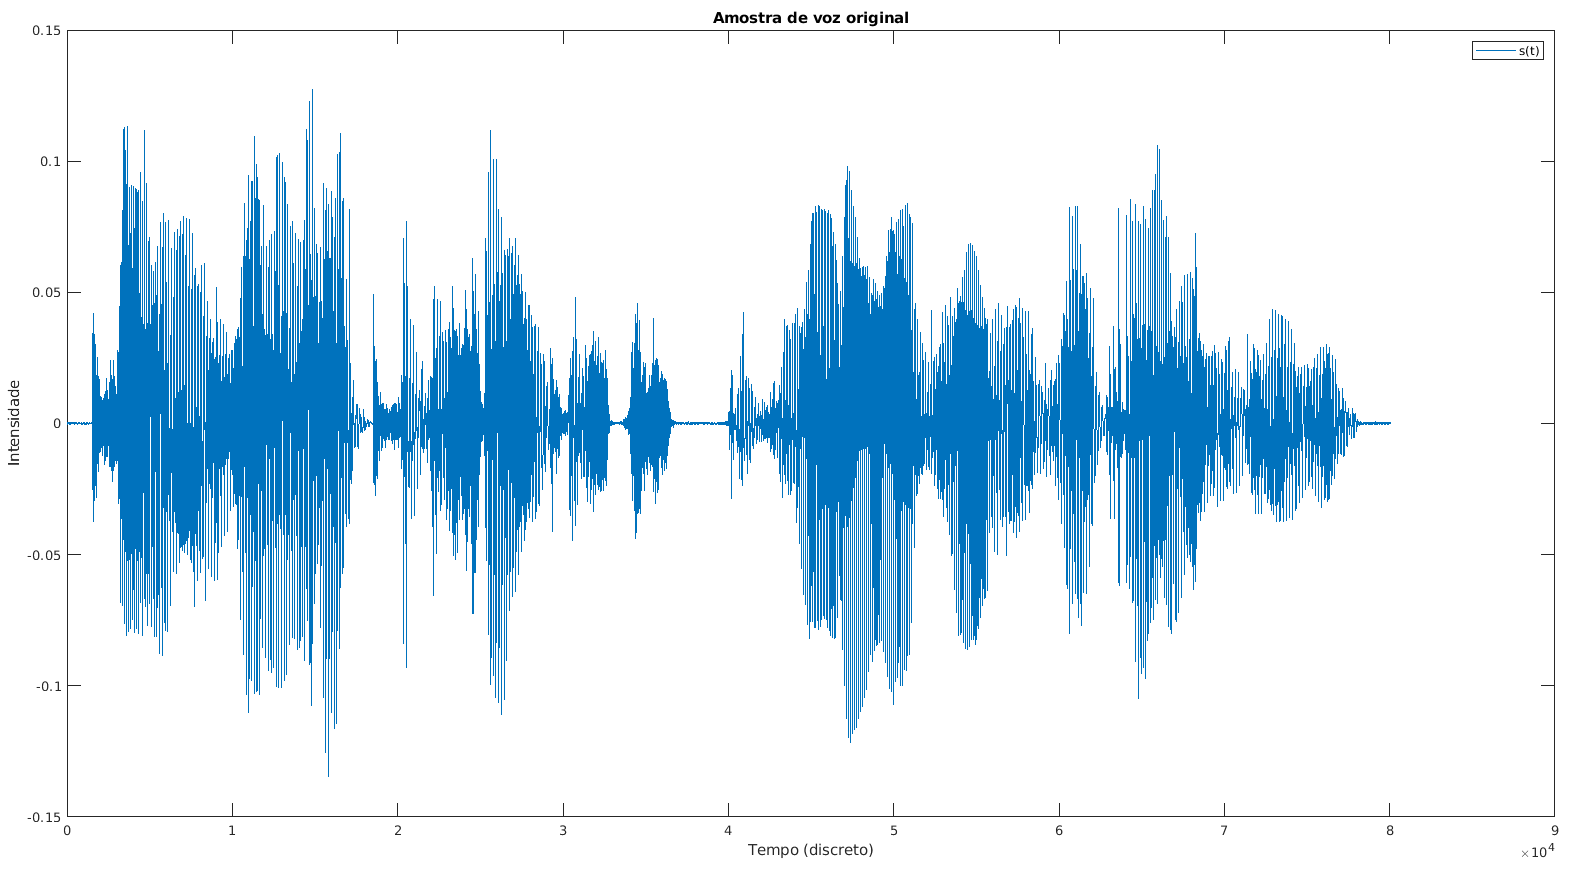
\includegraphics[scale=0.25]{voice-og-n5.png}
    \caption{Amostra de voz original.}
    \label{fig-a:voice-og-n5}
\end{figure} 

\begin{figure} [H]
    \centering
    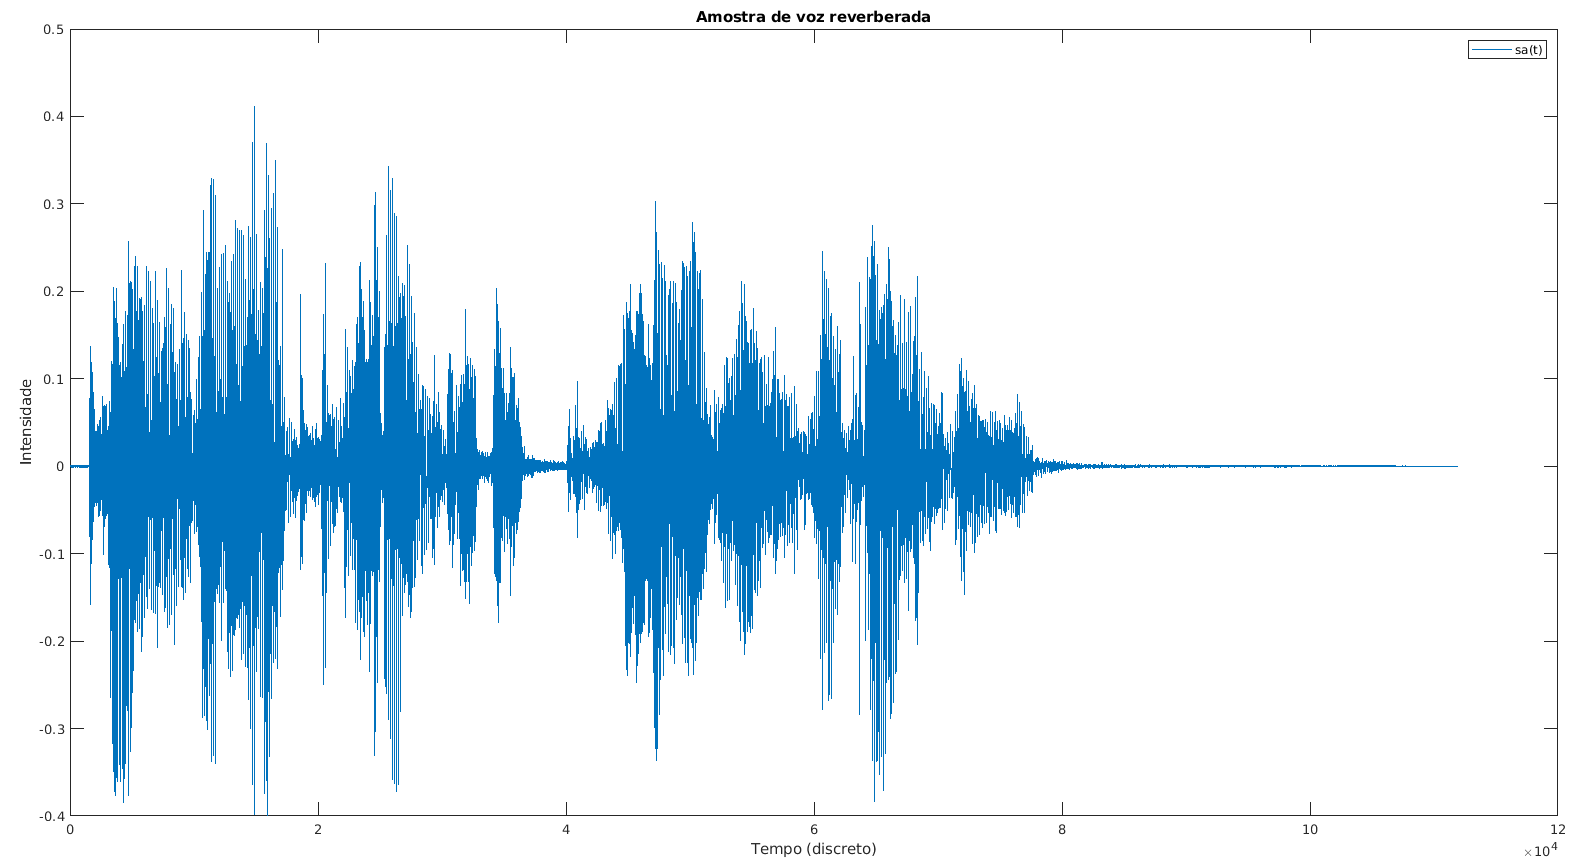
\includegraphics[scale=0.25]{voice-aug-n5.png}
    \caption{Amostra de voz reverberada com RIRSM.}
    \label{fig-a:voice-aug-n5}
\end{figure}

\begin{figure} [H]
    \centering
    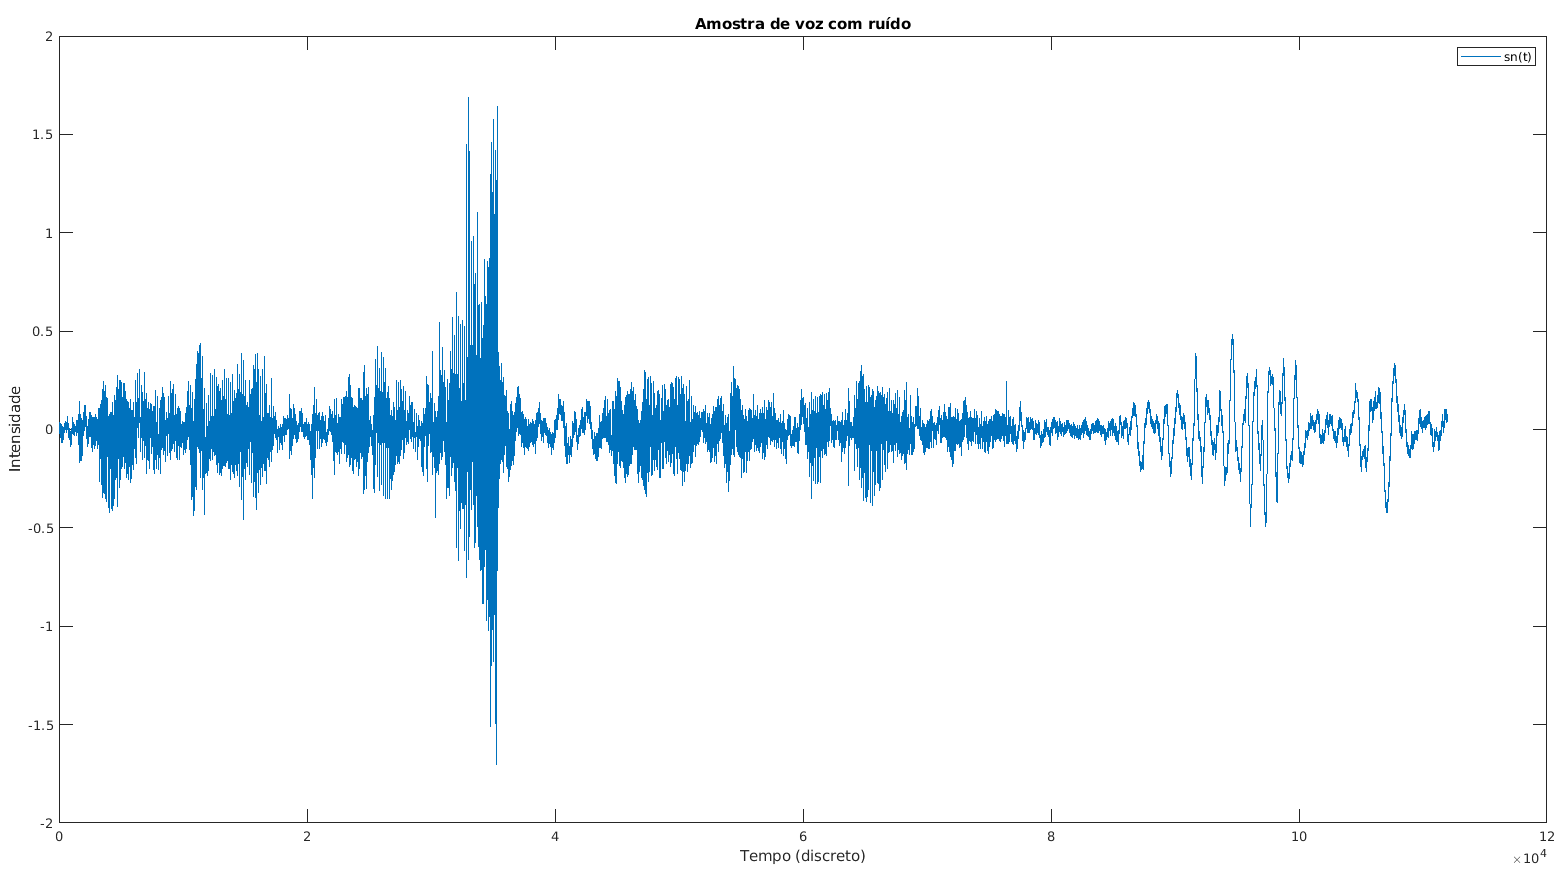
\includegraphics[scale=0.25]{voice-ns-n5.png}
    \caption{Amostra de voz em campo distante.}
    \label{fig-a:voice-ns-n5}
\end{figure}